% !TeX TS-program = XeLaTeX

% Commands for running this thesis:
% $ xelatex main
% $ bibtex8 -W -c cp1256fa maintext
% $  xindy -L persian -C utf8 -M texindy maintext
% $ xelatex maintext
% $ xelatex maintext
% End of Commands

%%%%%%%%%%%%%%
%% Welcome to Latex Template for IUST CE Thesis
%% The v0.8 quotes
%% The nearest star is 4.25 light-years from Earth which is why most wishes take at least 9 years to come true :)
%%%%%%%%%%%%%%% 

%%%
%%% خوش آمدید!
% قالب پایان‌نامه‌های کارشناسی، ارشد و دکتری، دانشگاه علم و صنعت ایران، دانشکده مهندسی کامپیوتر، آماده شده با استفاده از کلاس IUST-Thesis.
% نــگارش 0.9 توسط مرتضی ذاکری نصرآبادی - اردیبهشت 1399
% نــگارش 0.8 توسط مرتضی ذاکری نصرآبادی - مهر 1398
% نــگارش 0.7 توسط مرتضی ذاکری نصرآبادی  - تیر 1397
% - نــگارش 0.7 براساس نگارش 0.6 دکتر محمود امین طوسی آماده شده است.
% - این نسخه بر اساس نگارش 0.7 ساخته شده است. 

%استفاده از قالب با رعایت حقوق نشر، آزاد است.
%%% 
% نگارش 0.6 توسط محمود امین‌طوسی، دانشگاه تربیت معلم سبزوار، http://profsite.sttu.ac.ir/mamintoosi/
% گروه پارسی‌لاتک  http://www.parsilatex.com
% نگارش 0.6، بر اساس نسخه‌ 0.4 از کلاس Tabriz_Thesis آقای وحید دامن‌افشان آماده شده است؛ رجوع شود به: http://damanafshan.tk
%%%%%%%%%%%%%%%%%%%%%%%%%%%%% 


%%% تغییرات 
% نسخه 0.8:
% - افزودن بسته \usepackage{verbatim} برای مدیریت توضیحات متن
% - بروزرسانی گرافیک و فونت صفحه عنوان فارسی
% - متناسب سازی برای رساله دکتری

% نسخه 0.7: 
% - بروز رسانی بسته‌ها، اصلاح مشکلات مربوط به عدم تطابق با texlive2018 و اصلاحات جزئی دیگر. پرسش و پاسخ و ارسال دیدگاه‌ها:  
% http://m-zakeri.github.io
% -ریز تغییرات به شرح زیر است:
% -- اضافه شدن بسته‌(ها)ی مدیریت واژگان و کوته‌نوشت‌ها به صورت خودکار 
% -- اضافه شدن بسته‌ها و تنظیمات مربوط به درج کدمنبع برنامه‌ها در متن پایان نامه.
% -- اضافه شدن بسته‌ها و تنظیمات مروبط به درج الگوریتم‌ در استانداردهای نوشتاری نوین در متن پایان‌نامه.
% -- اضافه شدن بسته‌ها و تنظیمات مربوط به درج جدول در استانداردهای نوشتاری نوین در متن پایان‌نامه.
% -- اضافه شدن بسته‌ها و تنظیمات درج bookmark در خروجی.
% -- اضافه شدن بسته‌ها و تنظیمات درج صحیح پاورقی‌ها
% -- اضافه شدن بسته‌ها و تنظیمات مربوط به ایجاد نسخه‌های پیش‌نویس و نیز متن پس‌زمینه
% -- اضافه شدن بسته‌ها و تنظیمات مربوط به درج نقل قول‌های مستقیم و غیر مستقیم و epigraph
% -- اضافه شدن سایر بسته‌های مربوط به مدیریت فونت و استایل پایان‌نامه و ساختاربندی مجزای تصاویر و کدها (ارائه پارتیشن‌بندی استاندارد).

 
% نسخه 0.6:
% -- اصلاح مشکل بسته subfig 
%%%%%%%%%%%%%%%%%%%%%%%%%%%%


% -- اگر قصد نوشتن پروژه کارشناسی را دارید، در خط زیر به جای msc، کلمه bsc و اگر قصد نوشتن پروژه دکترا را دارید، کلمه phd را قرار دهید. کلیه تنظیمات لازم، به طور خودکار، اعمال می‌شود.
% -- اگر مایلید پایان‌نامه  دو رو باشد به جای oneside در خط زیر از twoside استفاده کنید.
\documentclass[twoside, openany, phd]{IUST-Thesis} % draft

% -- فایل settings.tex را مطالعه کنید. دستورات مربوط به فراخوانی بسته زی‌پرشین و دیگر بسته‌ها، در این فایل قرار دارد. بهتر است که با نحوه استفاده از آنها آشنا شوید.

%%
% Last update: 2024-07-10
%%
% در این فایل، دستورها و تنظیمات مورد نیاز، آورده شده است.
%%%%%%%%%%%%%%%%%%%%%%%%%%%%%%%%%%%%%
% دستوراتی که پوشه پیش‌فرض زیرفایل‌های tex را مشخص می‌کند.
%\makeatletter
%\def\input@path{{./tex/}}
%\makeatother
\RequirePackage{flafter}
\RequirePackage[bottom]{footmisc}
%\RequirePackage{enumerate}
\RequirePackage{enumitem}
\setlist[itemize]{noitemsep,  nolistsep}
% در ورژن جدید زی‌پرشین برای تایپ متن‌های ریاضی، این سه بسته، حتماً باید فراخوانی شود
\RequirePackage{amsthm, amsmath, amssymb, amsfonts}
%\RequirePackage{amssymb, amsmath, amsfonts}
\RequirePackage{thmtools}
%\RequirePackage{thmbox}


% بسته‌ای برای تنطیم حاشیه‌های بالا، پایین، چپ و راست صفحه
\RequirePackage[top=28mm, bottom=22mm, left=16mm, right=24mm]{geometry}
\RequirePackage[T1]{fontenc}
%\RequirePackage{titlesec}
\RequirePackage{setspace}
\RequirePackage{pdflscape}
%\RequirePackage{lscape}
\RequirePackage{titling}


%\RequirePackage{color}
\RequirePackage[x11names, usenames, dvipsnames, svgnames, table]{xcolor}

%\RequirePackage{bm}
\RequirePackage{verbatim}
%\RequirePackage{rotating}
%\RequirePackage{lettrine}
%\renewcommand{\LettrineTextFont}{}

% بسته‌‌ای برای ظاهر شدن شکل‌ها و تعیین آدرس تصاویر
\RequirePackage[final]{graphicx}
\graphicspath{{./figs/}}
\RequirePackage{caption}
%\RequirePackage{subcaption}
%\RequirePackage{subfig}

\RequirePackage{float}
\RequirePackage{xparse}
\RequirePackage{listing}
\RequirePackage[final]{listings}
\lstset{inputpath=./codes/}



\RequirePackage{soulutf8}

% بسته‌ای برای رسم کادر
%\RequirePackage{framed}  %%%%13990905
% بسته‌‌ای برای چاپ شدن خودکار تعداد صفحات در صفحه «معرفی پایان‌نامه»
\RequirePackage{lastpage}

\RequirePackage{cite}	% Add by Morteza %

% بسته‌ٔ لازم برای: ۱. تغییر شماره‌گذاری صفحات پیوست. ۲. تصحیح باگ آدرس وب حاوی '%' در مراجع
\RequirePackage{etoolbox}

\RequirePackage{comment}

%%%%%%%%%%%%%%%%%%%%%%%%%%%%%%%%%%%%
%%% دستورات وابسته به استیل مراجع:
%% اگر از استیل‌های natbib (plainnat-fa، asa-fa، chicago-fa) استفاده می‌کنید، خط زیر را فعال و بعدی‌اش را غیرفعال کنید.
%\RequirePackage{natbib}
%\newcommand{\citelatin}[1]{\cite{#1}\LTRfootnote{\citeauthor*{#1}}}
%\newcommand{\citeplatin}[1]{\citep{#1}\LTRfootnote{\citeauthor*{#1}}}
%% اگر از سایر استیل‌ها استفاده می‌کنید، خط بالا را غیرفعال و خط‌های زیر را فعال کنید.
\let\citep\cite
\let\citelatin\cite
\let\citeplatin\cite

\RequirePackage{bibentry}

%%%%%%%%%%%%
%\RequirePackage[nostamp]{draftwatermark}
% بررسی حالت پیش نویس
\RequirePackage{ifdraft}
\ifdraft
{%
% بسته‌ٔ ایجاد لینک‌های رنگی با امکان جهش
	\RequirePackage[unicode=true,pagebackref=true, colorlinks, linkcolor=blue, citecolor=red, bookmarks=true, final]{hyperref}
	%\RequirePackage{todonotes}
	%\RequirePackage[firstpage]{draftwatermark}
	\RequirePackage{draftwatermark}
	\SetWatermarkText{\ \ \ پیش‌نویس}
	\SetWatermarkScale{1.2}
}
{
	% اضافه کردن امکان ایجاد لینک به صفحه به جای عنوان در فهرست‌ها
    %SpringGreen4
    %LimeGreen
	\RequirePackage[unicode=true, pagebackref=false, colorlinks, linkcolor=Blue, citecolor=SpringGreen4, urlcolor=RoyalBlue4, bookmarks=true, linktocpage, breaklinks]{hyperref} %RoyalBlue1 % FireBrick
	%\RequirePackage[disable]{todonotes} % final without TODOs
	%\RequirePackage[firstpage]{draftwatermark}
	%\RequirePackage{draftwatermark}
	%\SetWatermarkColor[RGB]{240, 240, 245}
	%\SetWatermarkLightness{0.9813}
	%\SetWatermarkText{مرتـضی ‌ذاکــری}
	%\SetWatermarkText{\ \ \ پیش‌نویس}
	%\SetWatermarkScale{0.65}
}


\RequirePackage[obeyDraft]{todonotes}
\setlength{\marginparwidth}{2cm}

% تعیین مشخصات فایل PDF
\hypersetup{
	pdftitle={Measuring and Improving Testability of Software Systems Artifacts},
	pdfauthor={Morteza ZAKERI},
	pdfsubject={Ph.D. dissertation},
	pdfkeywords={Software artifacts; testability; covergaeability; software smell; automated refactoring; intelligent software engineering; testabilty-driven development.},
    pdfdirection={R2L}
}


%%%%%%%%%%%%
%%% تصحیح باگ: اگر در مراجع، آدرس وب حاوی '%' بوده و pagebackref فعال باشد، دستورات زیر باید بیایند:
%% برای استیل‌های natbib مثل plainnat-fa، asa-fa، chicago-fa
\makeatletter
\let\ORIG@BR@@lbibitem\BR@@lbibitem
\apptocmd\ORIG@BR@@lbibitem{\endgroup}{}{}
\def\BR@@lbibitem{\begingroup\catcode`\%=12 \ORIG@BR@@lbibitem}
\makeatother
%% برای سایر استیل‌ها
\makeatletter
\let\ORIG@BR@@bibitem\BR@@bibitem
\apptocmd\ORIG@BR@@bibitem{\endgroup}{}{}
\def\BR@@bibitem{\begingroup\catcode`\%=12 \ORIG@BR@@bibitem}
\makeatother
%%%%%%%%%%%%%%%%%%%%%%%%%%%%%%%%%%%%



% بسته‌ و دستوراتی برای ایجاد لینک‌های رنگی با امکان جهش
%\RequirePackage[pagebackref=false,colorlinks,linkcolor=blue,citecolor=purple]{hyperref}
% چنانچه قصد پرینت گرفتن نوشته خود را دارید، خط بالا را غیرفعال و  از دستور زیر استفاده کنید چون در صورت استفاده از دستور زیر‌‌، 
% لینک‌ها به رنگ سیاه ظاهر خواهند شد که برای پرینت گرفتن، مناسب‌تر است
%\RequirePackage[pagebackref=false]{hyperref}
% بسته‌ لازم برای تنظیم سربرگ‌ها
\RequirePackage{fancyhdr}
%\RequirePackage{setspace}
% بسته‌های لازم برای نوشتن الگوریتم
\RequirePackage{algorithm}
\RequirePackage{algorithmic}
% Add by Morteza %
%\RequirePackage[linesnumbered,ruled,vlined]{algorithm2e}
% بسته‌های لازم برای رسم بهتر جداول
\RequirePackage{tabulary}
\RequirePackage{tabularx}
%% Add by Morteza
\RequirePackage{multirow}
\RequirePackage{threeparttable}
\RequirePackage{fourier-otf} 
\RequirePackage{array}
\RequirePackage{makecell}  % I use this %
\RequirePackage{booktabs}
\RequirePackage{hhline}
 \RequirePackage{vcell}
 \RequirePackage{colortbl}
 \RequirePackage{arydshln}
%\RequirePackage{graphicx}

%%
% بسته‌های لازم برای رسم تنظیم بهتر شکل‌ها و زیرشکل‌ها
\RequirePackage[export]{adjustbox}
%\RequirePackage{subfigure}

%\RequirePackage[subfigure]{tocloft}
\RequirePackage{tocloft}
%\RequirePackage{subfig}
%\RequirePackage{caption}
%\RequirePackage{subcaption}

%%%%%%%%%%%%%%%%%%%%%%%%%%%%%%%%%%%%
% بسته‌ای برای رسم نمودارها و نیز صفحه مالکیت اثر
\RequirePackage{tikz}
\RequirePackage{tikzsymbols}
\usetikzlibrary{calendar,fpu}
% بسته‌ای برای ظاهر شدن «مراجع» و «نمایه» در فهرست مطالب
\RequirePackage[nottoc]{tocbibind}
% دستورات مربوط به ایجاد نمایه
\RequirePackage{makeidx}
\makeindex
%%% بسته ایجاد واژه‌نامه با xindy
\RequirePackage[xindy, acronym, nonumberlist=true]{glossaries}


%%%%%%%%%%%%%%%%%%%%%%%%%%
% Use the package sectsty to do change the headings, and xcolor to get the colour definitions.
\RequirePackage{sectsty}
%\titleformat{\chapter}[display]{\titlefont\Huge}{\chaptertitlename\ \tartibi{chapter}}{1em}{}
%\titleformat{\chapter}[display]
%{}{{\Huge \filright\chaptertitlename\ \thechapter}}
%{%30pt}{\filright}

\sectionfont{\fontsize{11}{13}\selectfont}
%\sectionfont{\fontsize{11}{13}\yagut}
%Coloring chapter{} and sections{}
%\chapterfont{\raggedleft}
\chapterfont{\color{DodgerBlue4}  \Huge\Huge \raggedleft}  % sets colour of chapters
\sectionfont{\color{DeepSkyBlue4}}  % sets colour of sections
\subsectionfont{\color{DeepSkyBlue3}}  % sets colour of sections

%% Set the font-size of Figure and Table captions
\DeclareCaptionFont{mysize}{\fontsize{10.5}{9.45}\yagut}
\captionsetup{font=mysize}

\captionsetup[figure]{labelfont={color=Brown4, bf}, textfont={color=DarkSlateGrey}} %DarkSlateGrey %darkgray
\captionsetup[table]{labelfont={color=Brown4, bf},  textfont={color=DarkSlateGray}}  %%Brown4 % Indigo

\RequirePackage{titlesec}
%\RequirePackage{indentfirst}
%% Set spacing
%\setlength{\textfloatsep}{\baselineskip}
\setlength{\textfloatsep}{4pt}
%\setlength{\parindent}{0pt}
 
\titlespacing*\section{0pt}{0pt plus 1pt minus 1pt}{0pt plus 1pt minus 1pt}
\titlespacing*\subsection{0pt}{0pt plus 1pt minus 1pt}{0pt plus 1pt minus 1pt}
\titlespacing*\subsubsection{0pt}{0pt plus 1pt minus 1pt}{0pt plus 1pt minus 1pt}
%
\setlength{\abovedisplayskip}{-1pt}
\setlength{\belowdisplayskip}{-1pt}

%% End of set spacing

%\setkomafont{title}{\huge \linespread{1.5}}%
\pretitle{\begin{center}\linespread{1.5}\huge }
\posttitle{\par\end{center}\vspace{0.5em}}



% بسته زیر باگ ناشی از فراخوانی بسته‌های زیاد را برطرف می‌کند.
\RequirePackage{morewrites}

%%%%%%%%%%%%%%%%%%%%%%%%%%
% فراخوانی بسته زی‌پرشین و تعریف قلم فارسی و انگلیسی
% قلم فارسی بازنویسی و قابل حمل شده است. امکان استفاده از چندین فونت فارسی مختلف در این قسمت فراهم شده است. برای استفاده نیازی به نصب بودن فونت ها روی رایانه خود ندارید.

%\RequirePackage[extrafootnotefeatures]{xepersian}
\RequirePackage{xepersian}

\settextfont[Path={./font/Niloofar/}, BoldFont={XBNiloofarBd.ttf}, ItalicFont={XBNiloofarIt.ttf}, BoldItalicFont={XBNiloofarBdIt.ttf}, Scale=1.05]{XBNiloofar.ttf}

\setlatintextfont[Scale=0.90]{Times New Roman}



%-----------------
%% https://github.com/persiantex/xepersian/issues/17
% this is a temporary fix as stated in https://github.com/persiantex/xepersian/issues/17#issuecomment-709956867
\ExplSyntaxOn
\cs_set_eq:NN
\etex_iffontchar:D
\tex_iffontchar:D
\cs_undefine:N \c_one
\int_const:Nn \c_one { 1 } 
\ExplSyntaxOff
%-----------------
% چنانچه می‌خواهید اعداد در فرمول‌ها، انگلیسی باشد، خط زیر را غیرفعال کنید
%\setdigitfont[Path={./font/Zar/}, BoldFont={XBZarBd.ttf}, ItalicFont={XBZarIt.ttf}, BoldItalicFont={XBZarBdIt.ttf}, Scale=1.0]{XBZar.ttf}
\setmathdigitfont[Path={./font/Zar/}, BoldFont={XBZarBd.ttf}, ItalicFont={XBZarIt.ttf}, BoldItalicFont={XBZarBdIt.ttf}, Scale=1.0]{XBZar.ttf}

% اگر می‌خواهید که اعداد با فونت یکان نمایش داده شوند خط بالا را غیر فعال کرده و خط زیر را فعال کنید.

%\setdigitfont[Path={./font/Yekan/}, BoldFont={XMYekanBd.ttf}, ItalicFont={XMYekanIt.ttf}, BoldItalicFont={XMYekanBdIt.ttf}, Scale=1.0]{XMYekan.ttf}%{Persian Modern}

% تعریف قلم‌های فارسی و انگلیسی برای استفاده در بعضی از قسمت‌های متن
\defpersianfont\niloofar[Path={./font/Niloofar/}, BoldFont={XBNiloofarBd.ttf}, ItalicFont={XBNiloofarIt.ttf}, BoldItalicFont={XBNiloofarBdIt.ttf}, Scale=1.0]{XBNiloofar.ttf}

\defpersianfont\zar[Path={./font/Zar/}, BoldFont={XBZarBd.ttf}, ItalicFont={XBZarIt.ttf}, BoldItalicFont={XBZarBdIt.ttf}, Scale=1.0]{XBZar.ttf}

\defpersianfont\yagut[Path={./font/Yagut/}, BoldFont={XBYagutBd.ttf}, ItalicFont={XBYagutIt.ttf}, BoldItalicFont={XBYagutBdIt.ttf}, Scale=1.0]{XBYagut.ttf}

\defpersianfont\titlefont[Path={./font/Titre/}, BoldFont={XBTitreShadow.ttf}, ItalicFont={XBTitreIt.ttf}, BoldItalicFont={XBTitreShadowIt.ttf}, Scale=1.0]{XBTitre.ttf}

\defpersianfont\iranic[Path={./font/Zar/XBZarOblique/}, BoldFont={XBZarObliqueBd.ttf}, Scale=1.10]{XBZarOblique.ttf}%Italic}%

\defpersianfont\nastaliq[Path={./font/IranNastaliq/}, Scale=1.50]{IranNastaliq.ttf}







% بسته زیر و متعاقباً دستورات ادامه آن، برای برای ریست کردن شماره پانویس‌ها در هر صفحه قرار داده شده است (به درخواست دکتر محمد عبداللهی ازگمی)

%\RequirePackage[perpage]{footmisc}
\RequirePackage{zref-perpage}
\zmakeperpage{footnote}

%\RequirePackage[rldocument]{bidi}
\RequirePackage{bidi}
\makeatletter
\@bidi@removefromreset{footnote}{chapter}
\makeatother


% راستچین شدن todonotes
\presetkeys{todonotes}{align=right, textdirection=righttoleft}{}
\makeatletter
\providecommand\@dotsep{5}
\def\listtodoname{فهرست کارهای باقیمانده}
\def\listoftodos{\noindent{\Large\vspace{10mm}\textbf{\listtodoname}}\@starttoc{tdo}}
\renewcommand{\@todonotes@MissingFigureText}{شکل}
\renewcommand{\@todonotes@MissingFigureUp}{شکل}
\renewcommand{\@todonotes@MissingFigureDown}{جاافتاده}
\makeatother
% دستوری برای حذف کلمه «چکیده»
%\renewcommand{\abstractname}{}
% دستوری برای حذف کلمه «abstract»
%\renewcommand{\latinabstract}{}
% دستوری برای تغییر نام کلمه «اثبات» به «برهان»
\renewcommand\proofname{\textbf{برهان}}
% دستوری برای تغییر نام کلمه «کتاب‌نامه» به «مراجع»
\renewcommand{\bibname}{مراجع}
% دستوری برای تعریف واژه‌نامه انگلیسی به فارسی
\newcommand\persiangloss[2]{#1\dotfill\lr{#2}\\}
% دستوری برای تعریف واژه‌نامه فارسی به انگلیسی 
\newcommand\englishgloss[2]{#2\dotfill\lr{#1}\\}
% تعریف دستور جدید «\پ» برای خلاصه‌نویسی جهت نوشتن عبارت «پروژه/پایان‌نامه/رساله»
\newcommand{\پ}{پروژه/پایان‌نامه/رساله}

%\newcommand\BackSlash{\char`\\}

%%%%%%%%%%%%%%%%%%%%%%%%%%
\SepMark{-}


% تعریف و نحوه ظاهر شدن عنوان قضیه‌ها، تعریف‌ها، مثال‌ها و ...
\declaretheorem[style=remark]{xyz}

\declaretheorem[
style=plain,
thmbox={style=S, bodystyle=\normalfont\noindent},
name=مسئله,
within=chapter,
]{problem}

%\declaretheorem[
%style=plain,
%thmbox={style=S, bodystyle=\normalfont\noindent},
%name=راه‌حل,
%]{solution}

\declaretheorem[
style=remark,
thmbox={style=M, bodystyle=\normalfont, headstyle=\itshape Remark \upshape\theremark},
name=Remark,
within=section,
qed=$\blacksquare$
]{remark}

%\newtheorem[L]{problem}{مسئله}[section]
%\theoremstyle{plain}
\theoremstyle{definition}
%\newtheoremstyle{sltheorem}
%{}                % Space above
%{}                % Space below
%{\slshape}        % Theorem body font % (default is "\upshape")
%{}                % Indent amount
%{\bfseries}       % Theorem head font % (default is \mdseries)
%{.}               % Punctuation after theorem head % default: no punctuation
%{ }               % Space after theorem head
%{}                % Theorem head spec

%\theoremstyle{sltheorem}
%\newtheorem{theorem}{Theorem}
%\declaretheorem[style=definition,name=Definition,qed=$\blacksquare$]{sol}
\renewcommand{\qedsymbol}{$\heartsuit$}
%\newtheorem{isolution}{راه‌حل پیشنهادی}
\newtheorem*{solution*}{راه‌حل پیشنهادی}
%\newenvironment{\solution}{\begin{\isolution}}{\qed \end{isolution}}

\newtheorem{definition}{تعریف}[section]
%\theoremstyle{theorem}
%\newtheorem{theorem}[definition]{قضیه}
%\newtheorem{lemma}[definition]{لم}
%\newtheorem{proposition}[definition]{گزاره}
%\newtheorem{corollary}[definition]{نتیجه}
%\newtheorem{remark}[definition]{ملاحظه}
%\theoremstyle{definition}
%\newtheorem{example}[definition]{مثال}

%\renewcommand{\theequation}{\thechapter-\arabic{equation}}
%\def\bibname{مراجع}
\numberwithin{algorithm}{chapter}
\def\listalgorithmname{فهرست الگوریتم‌ها}
\def\listfigurename{فهرست شکل‌ها}
\def\listtablename{فهرست جدول‌ها}



%%%%%%%%%%%%%%%%%%%%%%%%%%%%
% دستورهایی برای سفارشی کردن سربرگ صفحات
% \newcommand{\SetHeader}{
% \csname@twosidetrue\endcsname
% \pagestyle{fancy}
% \fancyhf{} 
% \fancyhead[OL,EL]{\thepage}
% \fancyhead[OR]{\small\rightmark}
% \fancyhead[ER]{\small\leftmark}
% \renewcommand{\chaptermark}[1]{%
% \markboth{\thechapter-\ #1}{}}
% }
%%%%%%%%%%%%
%\def\MATtextbaseline{1.5}
%\renewcommand{\baselinestretch}{\MATtextbaseline}
%\fancyhead[LE,RO]{\slshape \rightmark}
%\fancyhead[LO,RE]{\slshape \leftmark}
%\fancyfoot[C]{\thepage}
\doublespacing
%%%%%%%%%%%%%%%%%%%%%%%%%%%%%
% دستوراتی برای اضافه کردن کلمه «فصل» در فهرست مطالب

\newlength\mylenprt
\newlength\mylenchp
\newlength\mylenapp

\renewcommand\cftpartpresnum{\partname~}
\renewcommand\cftchappresnum{\chaptername~}
\renewcommand\cftchapaftersnum{:}

\settowidth\mylenprt{\cftpartfont\cftpartpresnum\cftpartaftersnum}
\settowidth\mylenchp{\cftchapfont\cftchappresnum\cftchapaftersnum}
\settowidth\mylenapp{\cftchapfont\appendixname~\cftchapaftersnum}
\addtolength\mylenprt{\cftpartnumwidth}
\addtolength\mylenchp{\cftchapnumwidth}
\addtolength\mylenapp{\cftchapnumwidth}

\setlength\cftpartnumwidth{\mylenprt}
\setlength\cftchapnumwidth{\mylenchp}	

\makeatletter
{\def\thebibliography#1{\chapter*{\refname\@mkboth
   {\uppercase{\refname}}{\uppercase{\refname}}}\list
   {[\arabic{enumi}]}{\settowidth\labelwidth{[#1]}
   \rightmargin\labelwidth
   \advance\rightmargin\labelsep
   \advance\rightmargin\bibindent
   \itemindent -\bibindent
   \listparindent \itemindent
   \parsep \z@
   \usecounter{enumi}}
   \def\newblock{}
   \sloppy
   \sfcode`\.=1000\relax}}


%اگر مایلید در شماره گذاری حرفی و ابجد به جای آ از الف استفاده شود دستورات زیر را فعال کنید.   
%\def\@Abjad#1{%
%  \ifcase#1\or الف\or ب\or ج\or د%
%           \or هـ\or و\or ز\or ح\or ط%
%           \or ی\or ک\or ل\or م\or ن%
%           \or س\or ع\or ف\or ص%
%           \or ق\or ر\or ش\or ت\or ث%
%            \or خ\or ذ\or ض\or ظ\or غ%
%            \else\@ctrerr\fi}
%
% \def\abj@num@i#1{%
%   \ifcase#1\or الف\or ب\or ج\or د%
%            \or هـ‍\or و\or ز\or ح\or ط\fi

%   \ifnum#1=\z@\abjad@zero\fi}   
%  
%   \def\@harfi#1{\ifcase#1\or الف\or ب\or پ\or ت\or ث\or

% ج\or چ\or ح\or خ\or د\or ذ\or ر\or ز\or ژ\or س\or ش\or ص\or ض\or ط\or ظ\or ع\or غ\or

% ف\or ق\or ک\or گ\or ل\or م\or ن\or و\or ه\or ی\else\@ctrerr\fi}

\makeatother


%%%%%%%%%%
% Packages add by Morteza Zakeri to support code snips M.Sc. Thesis 13970415


% بسته‌های مورد نیاز برای نوشتن کدها، رنگ‌آمیزی آنها و تعیین پوشهٔ کدها

\definecolor{mygreen}{rgb}{0,0.6,0}
\definecolor{mygray}{rgb}{0.2,0.2,0.2}
\definecolor{mymauve}{rgb}{0.58,0,0.82} 

%\ProvidesFile{listings-xepersian.def}[2014/07/17 v0.3 bilingual captions for listings package]
%\def\lstlistingname{\if@RTL else\ Listing\fi}
%\def\lstlistlistingname{\if@RTL  else\  Listings\fi}

\lstdefinestyle{myStyle}{ 
	backgroundcolor=\color{white},   % choose the background color; you must add \RequirePackage{color} or \RequirePackage{xcolor}; should come as last argument
	basicstyle=\ttfamily, % whole listing /w verbatim font
	breakatwhitespace=false,         % sets if automatic breaks should only happen at whitespace
	breaklines=true,                 % sets automatic line breaking
	captionpos=b,                    % sets the caption-position to bottom
	commentstyle=\color{mygreen},    % comment style
	deletekeywords={...},            % if you want to delete keywords from the given language
	escapeinside={\%*}{*)},          % if you want to add LaTeX within your code
	extendedchars=true,              % lets you use non-ASCII characters; for 8-bits encodings only, does not work with UTF-8
	frame=tb,	                     % adds a frame around the code
	lineskip=.095cm,                   % space between code lines
	keepspaces=true,                 % keeps spaces in text, useful for keeping indentation of code (possibly needs columns=flexible)
	keywordstyle=\color{blue},       % keyword style
	language=Octave,                 % the language of the code
	morekeywords={*,...},            % if you want to add more keywords to the set
	numbers=left,                    % where to put the line-numbers; possible values are (none, left, right)
	numbersep=3pt,                   % how far the line-numbers are from the code
	numberstyle=\tiny\color{mygray}\lr, % the style that is used for the line-numbers
	rulecolor=\color{black},         % if not set, the frame-color may be changed on line-breaks within not-black text (e.g. comments (green here))
	showspaces=false,                % show spaces everywhere adding particular underscores; it overrides 'showstringspaces'
	showstringspaces=false,          % underline spaces within strings only
	showtabs=false,                  % show tabs within strings adding particular underscores
	stepnumber=1,                    % the step between two line-numbers. If it's 1, each line will be numbered
	stringstyle=\ttfamily\color{mymauve},     % string literal style
	tabsize=2,	                     % sets default tabsize to 2 spaces
	title=\lstname,                  % show the filename of files included with \lstinputlisting; also try caption instead of title
	captionpos=b,
	captiondirection=RTL
}

\lstdefinestyle{myStyle2}{
	basicstyle=\ttfamily, % whole listing /w verbatim font
	keywordstyle=\color{blue}\bfseries, % bold black keywords
	identifierstyle=, % nothing happens
	commentstyle=\color{LimeGreen}, % green comments
	stringstyle=\ttfamily\color{red}, % red typewriter font for strings
	showstringspaces=false % no special string spaces
	breaklines=true,
	breakatwhitespace=false,
	numbers=right, % line number formats
	numberstyle=\footnotesize\lr,
	numbersep=-10pt,
	frame=single,
	captionpos=b,
	captiondirection=RTL
}

\lstset{style=myStyle} % command to set default style
%\def\listingsfont{\ttfamily}
\def\lstlistingname{\rl{برنامه}}


%\def\lstlistingname{\rl{تکه کد}}


% for numbering subsubsections
%\setcounter{secnumdepth}{3}
% to include subsubsections in the table of contents
%\setcounter{tocdepth}{3}




%% Set LTRfootnote number to persian
\makeatletter
\def\LTRfootnote{\@ifnextchar[\@xLTRfootnote{\stepcounter\@mpfn
        \protected@xdef\@thefnmark{\persianfont\thempfn}%
        \@footnotemark\@LTRfootnotetext}}
\makeatother


%\RequirePackage{hyperref}
\RequirePackage{csquotes}
\RequirePackage{epigraph}
\RequirePackage{etoolbox}
\newcommand{\epigraphcolor}{DarkKhaki}
\makeatletter
\newlength\epitextskip
\pretocmd{\@epitext}{\color{NavajoWhite4} \yagut\itshape }{}{} %DimGray
\makeatother
%
\newcommand{\epigraphrulecolor}{DarkKhaki}
\makeatletter
\renewcommand{\@epirule}{{\color{\epigraphrulecolor}\rule[.75ex]{\epigraphwidth}{\epigraphrule}}}
\makeatother
%

\setlength\epigraphwidth{0.80\linewidth}
\renewcommand{\epigraphsize}{\small}
\renewcommand{\epigraphflush}{flushleft}
\renewcommand{\sourceflush}{flushleft}
\renewcommand{\textflush}{flushepinormal}

%\RequirePackage{polyglossia}
%\RequirePackage[algo2e,linesnumbered,ruled,vlined]{algorithm2e}
\RequirePackage{textgreek}
\RequirePackage{booktabs}  % professional-quality tables
\RequirePackage{nicefrac}  % compact symbols for 1/2, etc.
\RequirePackage{microtype}  % microtypography
\RequirePackage{textcomp}
\RequirePackage[algo2e, ruled, linesnumbered, resetcount]{algorithm2e}
\def\HiLi{\leavevmode\rlap{\hbox to \hsize{\color{yellow!50}\leaders\hrule height .8\baselineskip depth .5ex\hfill}}}

%\RequirePackage[printwatermark]{xwatermark}
\RequirePackage{watermark}
%\RequirePackage{bm}
\RequirePackage{subcaption}
%\RequirePackage{multicol}
%\renewcommand\thesubfigure{\harfi{subfigure}}
\renewcommand{\thesubfigure}{\harfi{subfigure}}

%%%PDF setting
\RequirePackage[open, openlevel=1, atend]{bookmark}[2022/08/30]
\bookmarksetup{color=blue}
\bookmark[dest=titlefa]{سنجش و بهبود خودکار آزمون‌پذیری مصنوعات سیستم‌های نرم‌افزاری}

%\bookmark[dest=acknowledgement]{درباره نسخه پیش‌نویس}
%\bookmark[dest=acknowledgment]{قدردانی}
\bookmark[dest=abstractfa]{چکیده}
\bookmark[dest=tableofcontent]{فهرست مطالب}

% end of packages add by Morteza
%%%%%%%%%



%%% تنظیمات مربوط به بسته  glossaries
%%% تعریف استایل برای واژه نامه فارسی به انگلیسی، در این استایل واژه‌های فارسی در سمت راست و واژه‌های انگلیسی در سمت چپ خواهند آمد. از حالت گروه ‌بندی استفاده می‌کنیم، 
%%% یعنی واژه‌ها در گروه‌هایی به ترتیب حروف الفبا مرتب می‌شوند، مثلا:
%%% الف
%%% افتصاد ................................... Economy
%%% اشکال ........................................ Failure
%%% ش
%%% شبکه ...................................... Network

\newglossarystyle{myFaToEn}{%
	\renewenvironment{theglossary}{}{}
	\renewcommand*{\glsgroupskip}{\vskip 5mm}
	\renewcommand*{\glsgroupheading}[1]{\subsection*{\glsgetgrouptitle{##1}}}
	\renewcommand*{\glossentry}[2]{\noindent\glsentryname{##1}\dotfill\space \glsentrytext{##1}
		
	}
}

%% % تعریف استایل برای واژه نامه انگلیسی به فارسی، در این استایل واژه‌های فارسی در سمت راست و واژه‌های انگلیسی در سمت چپ خواهند آمد. از حالت گروه ‌بندی استفاده می‌کنیم، 
%% % یعنی واژه‌ها در گروه‌هایی به ترتیب حروف الفبا مرتب می‌شوند، مثلا:
%% % E
%%% Economy ............................... اقتصاد
%% % F
%% % Failure................................... اشکال
%% %N
%% % Network ................................. شبکه

\newglossarystyle{myEntoFa}{%
	%%% این دستور در حقیقت عملیات گروه‌بندی را انجام می‌دهد. بدین صورت که واژه‌ها در بخش‌های جداگانه گروه‌بندی می‌شوند، 
	%%% عنوان بخش همان نام حرفی است که هر واژه در آن گروه با آن شروع شده است. 
	\renewenvironment{theglossary}{}{}
	\renewcommand*{\glsgroupskip}{\vskip 5mm}
	\renewcommand*{\glsgroupheading}[1]{
		\begin{LTR} 
			\subsection*{\glsgetgrouptitle{##1}} 
		\end{LTR}
	}
	%%% در این دستور نحوه نمایش واژه‌ها می‌آید. در این جا واژه فارسی در سمت راست و واژه انگلیسی در سمت چپ قرار داده شده است، و بین آن با نقطه پر می‌شود. 
	\renewcommand*{\glossentry}[2]{\noindent\glsentrytext{##1}\dotfill\space \glsentryname{##1}
		
	}
}

%%% تعیین استایل برای فهرست اختصارات
\newglossarystyle{myAbbrlist}{%
	%%% این دستور در حقیقت عملیات گروه‌بندی را انجام می‌دهد. بدین صورت که اختصارات‌ در بخش‌های جداگانه گروه‌بندی می‌شوند، 
	%%% عنوان بخش همان نام حرفی است که هر اختصار در آن گروه با آن شروع شده است. 
	\renewenvironment{theglossary}{}{}
	\renewcommand*{\glsgroupskip}{\vskip 5mm}
	\renewcommand*{\glsgroupheading}[1]{\begin{LTR} \subsection*{\glsgetgrouptitle{##1}} \end{LTR}}
	%%% در این دستور نحوه نمایش اختصارات می‌آید. در این جا حالت کوچک اختصار در سمت چپ و حالت بزرگ در سمت راست قرار داده شده است، و بین آن با نقطه پر می‌شود. 
	\renewcommand*{\glossentry}[2]{\noindent\lr{\Glsentrylong{##1}}\dotfill\space \lr{\glsentrytext{##1}}
    
}
	%%% تغییر نام محیط abbreviation به فهرست اختصارات
	\renewcommand*{\acronymname}{\rl{فهرست کوته‌نوشت‌ها}}
}

%%% برای اجرا xindy بر روی فایل .tex و تولید واژه‌نامه‌ها و فهرست اختصارات و فهرست نمادها یکسری  فایل تعریف شده است.‌ Latex داده های مربوط به واژه نامه و .. را در این 
%%%  فایل‌ها نگهداری می‌کند. مهم‌ترین option‌ این قسمت این است که 
%%% عنوان واژه‌نامه‌ها و یا فهرست اختصارات و یا فهرست نمادها را می‌توانید در این‌جا مشخص کنید. 
%%% در این جا عباراتی مثل glg، gls، glo و ... پسوند فایل‌هایی است که برای xindy بکار می‌روند. 
\newglossary[glg]{english}{gls}{glo}{واژه‌نامه انگلیسی به فارسی}
\newglossary[blg]{persian}{bls}{blo}{واژه‌نامه فارسی به انگلیسی}
\makeglossaries
\glsdisablehyper
%%% تعاریف مربوط به تولید واژه نامه و فهرست اختصارات و فهرست نمادها
%%%  در این فایل یکسری دستورات عمومی برای وارد کردن واژه‌نامه آمده است.
%%%  به دلیل این‌که قرار است این دستورات پایه‌ای را بازنویسی کنیم در این‌جا تعریف می‌کنیم. 
\let\oldgls\gls
\let\oldglspl\glspl

\makeatletter

\renewrobustcmd*{\gls}{\@ifstar\@msgls\@mgls}
\newcommand*{\@mgls}[1] {\ifthenelse{\equal{\glsentrytype{#1}}{english}}{\oldgls{#1}\glsuseri{f-#1}}{\lr{\oldgls{#1}}}}
\newcommand*{\@msgls}[1]{\ifthenelse{\equal{\glsentrytype{#1}}{english}}{\glstext{#1}\glsuseri{f-#1}}{\lr{\glsentryname{#1}}}}

\renewrobustcmd*{\glspl}{\@ifstar\@msglspl\@mglspl}
\newcommand*{\@mglspl}[1] {\ifthenelse{\equal{\glsentrytype{#1}}{english}}{\oldglspl{#1}\glsuseri{f-#1}}{\oldglspl{#1}}}
\newcommand*{\@msglspl}[1]{\ifthenelse{\equal{\glsentrytype{#1}}{english}}{\glsplural{#1}\glsuseri{f-#1}}{\glsentryplural{#1}}}

\makeatother

\newcommand{\newword}[4]{
	\newglossaryentry{#1}     {type={english},name={\lr{#2}},plural={#4},text={#3},description={}}
	\newglossaryentry{f-#1} {type={persian},name={#3},text={\lr{#2}},description={}}
}

%%% بر طبق این دستور، در اولین باری که واژه مورد نظر از واژه‌نامه وارد شود، پاورقی زده می‌شود. 
%% Left to right footnote
%\defglsentryfmt[english]{\glsgenentryfmt\ifglsused{\glslabel}{}{\LTRfootnote{\glsentryname{\glslabel}}}}

%% Right to left footnote
\defglsentryfmt[english]{\glsgenentryfmt\ifglsused{\glslabel}{}{\footnote{\glsentryname{\glslabel}}}}

%%% بر طبق این دستور، در اولین باری که واژه مورد نظر از فهرست اختصارات وارد شود، پاورقی زده می‌شود.
%% Left to right footnote 
%\defglsentryfmt[acronym]{\glsentryname{\glslabel}\ifglsused{\glslabel}{}{\LTRfootnote{\glsentrydesc{\glslabel}}}}

%% Right to left footnote
\defglsentryfmt[acronym]{\glsentryname{\glslabel}\ifglsused{\glslabel}{}{\rl{\footnote{\lr{\glsentrydesc{\glslabel}}}}}}


%%%%%% ============================================================================================================


%%%%%
% Add by Morteza
%\usepackage{etoolbox}
%\makeatletter
%\apptocmd{\@gls@}{\shyam@index{#2}}{}{}
%\def\shyam@index#1{%
%	\expandafter\expandafter\expandafter\shyam@index@aux\csname glo@#1@index\endcsname\shyam@index
%}
%\def\shyam@index@aux#1?#2\shyam@index{\index{#1}}
%\makeatother
%%%%%



%%============================ دستور برای قرار دادن فهرست اختصارات 
\newcommand{\printabbreviation}{
	%\cleardoublepage
	%\phantomsection
	\baselineskip=.75cm
	%% با این دستور عنوان فهرست اختصارات به فهرست مطالب اضافه می‌شود.
	\phantomsection 
	\addcontentsline{toc}{chapter}{فهرست کوته‌نوشت‌ها}
	\setglossarystyle{myAbbrlist}
	%\begin{LTR}
		\Oldprintglossary[type=acronym]	
	%\end{LTR}
	\clearpage
}%

\newcommand{\printacronyms}{\printabbreviation}
%%% در این جا محیط هر دو واژه نامه را باز تعریف کرده ایم، تا اولا مشکل قرار دادن صفحه اضافی را حل کنیم، ثانیا عنوان واژه نامه ها را با دستور addcontentlist وارد فهرست مطالب کرده ایم.
\let\Oldprintglossary\printglossary
\renewcommand{\printglossary}{
	\let\appendix\relax
	%% تنظیم کننده فاصله بین خطوط در این قسمت
	\clearpage
	\phantomsection
	%% این دستور موجب این می‌شود که واژه‌نامه‌ها در  حالت دو ستونی نوشته شود. 
	\twocolumn{}
	%% با این دستور عنوان واژه‌نامه به فهرست مطالب اضافه می‌شود. 
	\addcontentsline{toc}{chapter}{واژه‌نامه فـارسی به انگلیسی}
	\setglossarystyle{myFaToEn}
	\Oldprintglossary[type=persian]
	\clearpage
	%\phantomsection
	%% با این دستور عنوان واژه‌نامه به فهرست مطالب اضافه می‌شود. 
	\addcontentsline{toc}{chapter}{واژه‌نامه انگلیسی به فـارسی}
	\setglossarystyle{myEntoFa}
	%\begin{LTR}
		\Oldprintglossary[type=english]
	%\end{LTR}
	
	\onecolumn{}
}%
%%%%%%
% !TeX root=z-main.tex
% !TeX TS-program = XeLaTeX
% !TEX spellcheck = fa

%%
% My Thesis Acronyms
%%

%% Chapter1
\newacronym{MOST}{MOST}{Modern Open Scientific / Standard Templates}
\newacronym{SUT}{SUT}{software under test}
\newacronym{NLP}{NLP}{natural language processing}
\newacronym{SDLC}{SDLC}{software development life cycle}
\newacronym{ASE}{ASE}{automated software engineering}
\newacronym{EaASE}{EaASE}{empirical and automated software engineering}

%% Chapter2
\newacronym{AST}{AST}{abstract syntax tree}

%% Chapter3
%\newacronym{AFL}{AFL}{\lr{American Fuzzy Lop}}
\newacronym{TFIDF}{TF-IDF}{term frequenc-inverse document frequency}

%% Chapter4
\newacronym{ASCII}{ASCII}{american standard code for information interchange}

%% Chapter5
\newacronym{SOU}{SOU}{single object update}


%% Chapter6
\newacronym{GenerativeAdversarialNetwork}{GAN}{generative adversarial network}
\newacronym{CAN}{CAN}{creative adversarial networks}

% !TeX root=z-main.tex
% !TeX TS-program = XeLaTeX
% !TEX spellcheck = fa
%glassory

%%
% CS Glossary (Universal glassory).
% To collect a complete reference, please do not remove any word and instead comment them.
%%

%%
% جستجوی واژه‌های مصوّب فرهنگستان:
% https://wiki.apll.ir/word/index.php/Paradigm
%%

%%% Chapter1

%% Problem statement glassory
\newword{divide-and-conquer}{divide and conquer}{تقسیم و غلبه}{تقسیم و غلبه}
\newword{software-testing}{software testing}{آزمون ‌نرم‌افزار}{آزمون‌های نرم‌افزار}
\newword{test-data-generation}{test data generation}{تولید داده آزمون}{تولید داده‌های آزمون}
\newword{debugging}{debugging}{اشکال‌زدایی}{اشکال‌زدایی}
\newword{fault-localization}{fault localization}{مکان‌یابی خطا}{مکان‌یابی خطاها}
\newword{repair}{repair}{ترمیم}{ترمیم‌ها}
\newword{side-effect}{side effect}{تأثیر جانبی}{تأثیرات جانبی}
\newword{alias-name}{alias name}{اسم مستعار}{اسامی مستعار}
\newword{testability}{testability}{آزمون‌پذیری}{قابلیت‌ آزمون}

\newword{clean-code}{clean code}{‌کدِ پاک}{کدهای پاک}
\newword{refactoring}{refactoring}{بازآرایی}{بازآرایی‌ها}

\newword{source-code}{source code}{کدِ منبع}{کدهای منبع}
\newword{design}{design}{طراحی}{طراحی‌ها}
\newword{requirement}{requirement}{نیازمندی}{نیازمندی‌ها}

\newword{unit-test}{unit test}{آزمون واحد}{آزمون‌ واحد‌ها}
\newword{module-test}{module test}{آزمون پیمانه}{آزمون پیمانه‌ها}
\newword{integration-test}{integration test}{آزمون یکپارچگی}{آزمون‌های یکپارچگی}
\newword{system-test}{system test}{آزمون سیستم}{آزمون سیستم‌ها}
\newword{acceptance-test}{acceptance test}{آزمون پذیرش}{آزمون پذیرش}
\newword{developer-testing}{developer testing}{آزمون توسعه‌دهنده}{آزمون توسعه‌دهنده}
\newword{regression-testing}{regression testing}{آزمون رگرسیون}{آزمون رگرسیون}

\newword{quality-attribute}{quality attribute}{صفت کیفیت}{صفات کیفیت}
\newword{internal-quality-attribute}{internal quality attribute}{صفت کیفیت داخلی}{صفات کیفیت داخلی}
\newword{external-quality-attribute}{external quality attribute}{صفت کیفیت خارجی}{صفات کیفیت خارجی}

\newword{search-based}{search-based}{مبتنی بر جست‌و‌جو}{مبتنی بر جست‌وجو}
\newword{evolutionary}{evolutionary}{تکاملی}{تکاملی}
\newword{meta-heuristic}{meta-heuristic}{فرااکتشافی}{فرااکتشافی}
\newword{objective-function}{objective-function}{تابع هدف}{توابع هدف}

\newword{coverage}{coverage}{پوشش}{پوشش‌ها}
\newword{coverage-criteria}{coverage criteria}{معیارهای پوشش}{معیارهای پوشش}
\newword{symbolic-execution}{symbolic execution}{اجرای نمادین}{اجراهای نمادین}
\newword{dynamic-symbolic-execution}{dynamic symbolic execution}{اجرای نمادینِ پویا}{اجراهای نمادینِ پویا}
\newword{concolic-execution}{concolic execution}{اجرای واقعی-نمادین}{اجراهای واقعی-نمادین}
\newword{tester}{tester}{آزمون‌گر}{آزمون‌گرها}

\newword{single-responsibility-principle}{single responsibility pronciple}{اصل تک مسئولیتی}{اصل تک مسئولیتی}
\newword{dependency-injection}{dependency-injection}{تزریق وابستگی}{تزریق وابستگی}
\newword{design-pattern}{design pattern}{الگوی طراحی}{الگوهای طراحی}
\newword{factory}{factory}{کارخانه}{کارخانه}
\newword{polymorphism}{polymorphism}{چندریختی}{چندریختی}

\newword{long-method}{long method}{تابع طولانی}{توابع طولانی}
\newword{large-class}{large class}{کلاس بزرگ}{کلاس‌های بزرگ}
\newword{extract-method}{extract method}{استخراج تابع}{استخراج توابع}
\newword{extract-class}{extract class}{استخراج کلاس}{استخراج کلاس‌ها}
\newword{move-method}{move method}{انتقال تابع}{انتقال تابع}
\newword{move-class}{move class}{انتقال کلاس}{انتقال کلاس‌ها}

\newword{dependency-graph}{dependency graph}{گراف وابستگی}{گراف وابستگی‌ها}
\newword{component}{component}{مؤلفه}{مؤلفه‌ها}
\newword{module}{module}{پیمانه}{پیمانه‌ها}
\newword{modularity}{modularity}{پیمانگی}{پیمانگی}
\newword{cohesion}{cohesion}{چسبندگی}{چسبندگی}
\newword{coupling}{coupling}{اتصال}{اتصال}

\newword{reliability}{reliability}{قابلیت اطمینان}{قابلیت اطمینان}
\newword{understandability}{understandability}{قابلیت درک}{قابلیت درک}
\newword{changeability}{changeability}{قابلیت تغییر}{قابلیت تغییر}
\newword{reusability}{reusability}{قابلیت استفاده مجدد}{قابلیت استفاده مجدد}
\newword{maintainability}{maintainability}{قابلیت نگه‌داشت}{قابلیت نگه‌داشت}

\newword{sequence}{sequence}{توالی}{توالی‌ها}
\newword{optimum}{optimum}{بهینه}{بهینه}
\newword{feasible}{feasible}{امکان‌پذیر}{امکان‌پذیر}

\newword{software-smell}{software smell}{بوی نرم‌افزار}{بوهای نرم‌افزار}
\newword{code-smell}{code smell}{بوی کد}{بوی کد}
\newword{design-smell}{design smell}{بوی طراحی}{بوی طراحی}
\newword{architecture-smell}{architecture smell}{بوی معماری}{بوهای معماری}
\newword{test-smell}{test smell}{بوی آزمون}{بوهای آزمون}
\newword{requirement-smell}{requirement smell}{بوی نیازمندی}{بوهای نیازمندی}
\newword{smelly-code}{smelly code}{کد بودار}{کدهای بودار}
\newword{smelly-word}{smelly word}{واژه بودار}{واژه‌های بودار}

\newword{polysemy}{polysemy}{چندمعنایی}{چندمعنایی}
\newword{subjective-language}{subjective-language}{زبان موضوعی}{زبان موضوعی}
\newword{non-verifiable-term}{non-verifiable term}{اصطلاح غیرقابل درستی‌یابی}{اصطلاحات غیرقابل درستی‌یابی}
\newword{ambiguous}{ambiguous}{مبهم}{مبهم}
\newword{superlative}{superlative}{صفت عالی}{صفات عالی}
\newword{comparative}{comparative}{صفت تفضیلی}{صفات تفضیلی}
\newword{vague-pronouns}{vague pronouns}{ضمیر مبهم}{ضمیر مبهم}
\newword{uncertain-verbs}{uncertain-verbs}{فعل نامعیّن}{افعال نامعیّن}

\newword{criteria}{criteria}{معیار}{معیارها}
\newword{metric}{metric}{متریک}{متریک‌ها}
\newword{measure}{measure}{سنجه}{سنجه‌ها}

%% Related work glassory
\newword{cyclomatic-complexity}{cyclomatic complexity}{پیچیدگی حلقوی}{پیچیدگی حلقوی}
\newword{test-adequacy-criteria}{test adequacy criteria}{معیار کفایت آزمون}{معیارهای کفایت آزمون}

\newword{controllability}{controllability}{کنترل‌پذیری}{کنترل‌پذیری}
\newword{observability}{observability}{مشاهده‌پذیری}{مشاهده‌پذیری}
\newword{testability-transformation}{testability transformation}{تبدیل آزمون‌پذیری}{تبدیل آزمون‌پذیری}
\newword{user-friendly}{user friendly}{کاربر پسند}{کاربر پسند}
\newword{verification}{verification}{درستی‌یابی}{درستی‌یابی}
\newword{validation}{validation}{اعتبارسنجی}{اعتبارسنجی}

\newword{reverse-engineering}{reverse engineering}{مهندسی معکوس}{مهندسی معکوس}

\newword{coveragability}{coveragability}{پوشش‌پذیری}{پوشش‌پذیری}
\newword{code-coverage}{code coverage}{پوشش کد}{پوشش کد}
\newword{statement-coverage}{statement coverage}{پوشش دستور}{پوشش دستور}
\newword{branch-coverage}{branch coverage}{پوشش شاخه}{پوشش شاخه}
\newword{test-suite}{test suite}{مجموعه آزمون}{مجموعه‌های آزمون}

\newword{warm-start}{warm start}{شروع گرم}{شروع گرم}
\newword{cold-start}{cold start}{شروع سرد}{شروع سرد}

\newword{multi-objective}{multi objective}{چند هدفه}{چند هدفه}
\newword{many-objective}{many objective}{چندین هدفه}{چندین هدفه}

\newword{remodularization}{remodularization}{پیمانه‌سازی مجدد}{پیمانه‌سازی‌های مجدد}
\newword{restructuring}{restructuring}{تجدید ساختار}{تجدید ساختار}
\newword{developer-experience}{developer experience}{تجربه توسعه‌دهنده}{تجربه توسعه‌دهندگان}
%%
\newword{requirement-clarity}{requirement clarity}{وضوح نیازمندی}{وضوح نیازمندی}
\newword{clean-requirement}{claen requirement}{نیازمندی پاک}{نیازمندی‌های پاک}
\newword{word-embedding}{word embedding}{تعبیه‌واژه}{تعبیه‌واژه}

\newword{requirement-refactoring}{requirement refactoring}{بازآرایی نیازمندی}{بازآرایی نیازمندی‌ها}
\newword{semi-automated}{semi-automated}{نیمه‌خودکار}{نیمه‌خودکار}
\newword{fully-automated}{fully automated}{‌خودکار}{‌خودکار}

\newword{object-oriented}{object-oriented}{شیء‌گرا}{شی‌ءگرایی}
\newword{aspect-oriented}{aspect-oriented}{جنبه‌گرا}{جنبه‌گرا}
\newword{service-oriented}{service-oriented}{سرویس‌گرا}{سرویس‌گرا}
\newword{structural}{structured}{ساخت‌یافته}{ساخت‌یافته}

\newword{static-analysis}{static-analysis}{تحلیل ایستا}{تحلیل‌های ایستا}
\newword{dynamic-analysis}{dynamic-analysis}{تحلیل پویا}{تحلیل‌های پویا}

\newword{safety-critical-system}{safety critical system}{سیستم‌ حساس به ایمنی}{سیستم‌های حساس به ایمنی}


%\gls{refactoring}

%\newword{FuzzTesting}{fuzz testing}{آزمون فازی}{آزمون فازی}
%\newword{Monitor}{monitor}{پایش}{پایش}

%\newword{Vulnerability}{vulnerability}{آسیب‌پذیری}{آسیب‌پذیری‌ها}
%\newword{Malformed}{malformed}{بدشکل}{بدشکل}
\newword{test-case}{test case}{آزمایه}{آزمایه‌‌ها}
\newword{test-data}{test data}{داده آزمون}{داده‌های آزمون}
\newword{test-double}{test double}{همزاد آزمون}{ همزدا آزمون}

\newword{parser}{parser}{تجزیه‌گر}{تجزیه‌گرها}

%\newword{MagicByte}{magic bytes}{بایت جادویی}{بایت‌های جادویی}
%\newword{Marker}{markers}{نشان‌گر}{نشان‌گرها}
\newword{parse}{parse}{تجزیه}{تجزیه}
\newword{render}{render}{پرداخت}{پرداخت}

%\newword{MemoryCorruption}{memory corruption}{فساد حافظه}{فساد حافظه}
%\newword{Metadata}{metadata}{فراداده}{فراداده}

%\newword{Ransomware}{ransomware}{باج‌افزار}{باج‌افزارها}
%\newword{Attacker}{attacker}{مهاجم}{مهاجمان}

%\newword{ExceptionHandling}{exception handling}{کنترل استثنا}{کنترل استثنا}
%\newword{InternetOfThings}{internet of things}{اینترنت اشیاء}{اینترنت اشیاء}


%%%%%%%%%%%%%%%%%%%%%%%%%%%%%%
%% Chapter2
\newword{fault}{fault}{خطا}{خطاها}
\newword{error}{error}{اشکال}{اشکال‌ها}
\newword{failure}{failure}{خرابی}{خرابی‌ها}
\newword{specification}{specification}{مشخصه}{مشخصه‌ها}
\newword{dependability}{dependability}{اتکاپذیری}{اتکاپذیری}
\newword{undecidable}{undecidable}{تصمیم‌ناپذیر}{تصمیم‌ناپذیر}

\newword{InputSpacePartitioning}{input space partitioning}{افراز فضای ورودی}{افراز فضای ورودی}
\newword{GraphCoverage}{graph coverage}{پوشش گراف}{پوشش گراف}
\newword{LogicCoverage}{logic coverage}{پوشش منطق}{پوشش منطق}
\newword{SyntaxBasedCoverage}{syntax-based coverage}{پوشش ساختار نحوی}{پوشش ساختار نحوی}

\newword{RecognizerProgram}{recognizer program}{برنامه شناسنده}{برنامه شناسنده}
\newword{GeneratorProgram}{generator program}{برنامه مولد}{برنامه مولد}

\newword{line-coverage}{line coverage}{پوشش خط}{پوشش خط}
\newword{partial-line-coverage}{partial line coverage}{پوشش خط جزئی}{پوشش خط جزئی}
\newword{basic-block}{basic block}{بلوک پایه}{بلوک پایه}
\newword{basic-block-coverage}{basic block coverage}{پوشش بلوک پایه}{پوشش بلوک پایه}
\newword{path-coverage}{path coverage}{پوشش مسیر}{پوشش مسیر}
\newword{domain-coverage}{domain coverage}{پوشش دامنه}{پوشش دامنه}
\newword{Instrumenting}{instrumenting}{ابزارگذاری}{ابزارگذاری}

\newword{software-sizing}{software sizing}{اندازه نرم‌‌افزار}{اندازه نرم‌افزار}
\newword{parse-tree}{parse tree}{درخت تجزیه}{درخت تجزیه}
\newword{symbol-table}{symbol table}{جدول نماد}{جدول نمادها}
\newword{class-diagram}{class diagram}{نمودار کلاس}{نمودارهای کلاس}

\newword{objective}{objective}{عینی}{عینی}

\newword{anti-pattern}{anti-pattern}{ضد الگو}{ضد الگو}
\newword{technical-debt}{technical debt}{بدهی فنی}{بدهی‌های فنی}
\newword{code-debt}{test debt}{بدهی کد}{بدهی‌های کد}
\newword{design-debt}{design debt}{بدهی طراحی}{بدهی‌های طراحی}
\newword{test-debt}{test debt}{بدهی آزمون}{بدهی‌های آزمون}

\newword{roll-back}{roll-back}{بازگرد}{بازگردها}
\newword{anomally-detection}{anomally detection}{تشخیص ناهنجاری}{تشخیص ناهنجاری}

\newword{imbalanced}{imbalanced}{نامتوازن}{نامتوازن}


\newword{software-analytics}{software-analytics}{واکاوش نرم‌افزار}{واکاوش نرم‌افزار}
\newword{data-driven}{data-driven}{داده‌رانه}{داده‌رانه}
\newword{data-science}{data-science}{علم داده‌ها}{علم ‌داده‌ها}

\newword{representation}{representation}{بازنمایی}{بازنمایی}
\newword{concept}{concept}{مفهوم}{مفاهیم}
\newword{supervised}{supervised}{بانظارت}{بانظارت}
\newword{supervised-learning}{supervised learning}{یادگیری بانظارت}{یادگیری بانظارت}
\newword{unsupervised-learning}{unsupervised learning}{یادگیری بدون‌ نظارت}{یادگیری بودن ‌نظارت}
\newword{semi-supervised-learning}{semi-supervised learning}{یادگیری نیمه‌ نظارتی}{یادگیری بودن ‌نظارتی}
\newword{reinforcement-learning}{reinforcement learning}{یادگیری تقویتی}{یادگیری تقویتی}

\newword{multi-agent-learning}{multi-agent learning}{یادگیری چند عاملی}{یادگیری چند عاملی}

\newword{label}{label}{برچسب}{برچسب}
\newword{task}{task}{وظیفه}{وظایف}
\newword{regression}{regression}{رگرسیون}{رگرسیون‌ها}
\newword{classification}{classification}{طبقه‌بندی}{‌طبقه‌بندی‌ها}
\newword{clustering}{clustering}{خوشه‌بندی}{خوشه‌بندی‌ها}


\newword{lemmatization}{lemmatization}{بن واژه‌سازی}{بن ‌واژه‌سازی}
\newword{stemming}{stemming}{ریشه‌یابی}{ریشه‌یابی}


%% Not used in proposal
\newword{ShortCircuit}{short circuit}{مدار کوتاه}{مدار کوتاه}

\newword{BlackBox}{black box}{جعبه سیاه}{جعبه سیاه}
\newword{WhiteBox}{white box}{جعبه سفید}{جعبه سفید}
\newword{GrayBox}{gray box}{جعبه خاکستری}{جعبه خاکستری}

\newword{StressTesting}{stress testing}{آزمون فشار}{آزمون فشار}
\newword{Fuzzer}{fuzzer}{فازر}{فازر}
\newword{MutationBased}{mutation based}{مبتنی بر جابه‌جایی}{مبتنی بر جابه‌جایی}

\newword{GenerationBased}{generation based}{مبتنی بر تولید}{مبتنی بر تولید}
\newword{SampleInput}{sample input}{ورودی نمونه}{ورودی نمونه}
\newword{InputData}{input data}{داده ورودی}{داده ورودی}
\newword{Valid}{Valid}{معتبر}{معتبر}
\newword{InitialSeed}{initial seed}{دانه اولیه}{دانه‌های اولیه}
\newword{GenerativeModel}{generative model}{مدل مولد}{مدل‌های مولد}
\newword{Module}{module}{پیمانه}{پیمانه‌ها}
\newword{FileFormatFuzzer}{file format fuzzer}{فازر قالب فایل}{فازر قالب فایل}

\newword{PenetrationTesting}{penetration testing}{آزمـون نفوذ}{آزمون‌های نفوذ}
\newword{RobustnessTesting}{robustness testing}{آزمون قدرت‌مندی}{آزمون‌های قدرت‌مندی}
\newword{SecurityTesting}{security testing}{آزمون امنیت}{آزمون‌های امنیت}

\newword{Exploit}{exploit}{بهره‌برداری}{بهره‌برداری}
\newword{Buffer}{buffer}{میانگیر}{میانگیرها}

\newword{DeepLearning}{deep learning}{یادگیری ژرف}{یادگیری ژرف}
\newword{NeuralNetwork}{neural network}{شبکه عصبی}{شبکه‌های عصبی}
\newword{DeepNeuralNetwork}{deep neural network}{شبکه عصبی ژرف}{شبکه عصبی ژرف}
\newword{FeedforwardNeuralNetwork}{feed-forward neural network}{شبکه عصبی روبه‌جلو}{شبکه‌های عصبی روبه‌جلو}

\newword{HiddenLayer}{hidden layer}{لایه پنهان}{لایه‌های پنهان}
\newword{Neuron}{neuron}{عصب}{عصب‌ها}
\newword{Unit}{unit}{واحد}{واحدها}
\newword{Bias}{bias}{بایاس}{بایاس}
\newword{ActivationFunction}{activation function}{تابع انگیزش}{توابع انگیزش}

\newword{TrainingSet}{training set}{مجموعه آموزش}{مجموعه‌های آموزش}
\newword{TestSet}{test set}{مجموعه آزمون}{مجموعه‌های آزمون}
\newword{ValidationSet}{validation set}{مجموعه ارزیابی}{مجموعه‌های ارزیابی}

\newword{ForwardPass}{forward pass}{گذرِجلو}{گذرِجلو}
\newword{ErrorFunction}{error function}{تابع خطا}{تابع خطا}
\newword{CostFunction}{cost function}{تابع هزینه}{توابع هزینه}
\newword{MeanAbsoluteError}{mean absolute error}{خطای مطلق میانگین}{خطای مطلق میانگین}
\newword{MeanSquaredError}{mean squared error}{خطای میانگین مربعات}{خطای میانگین مربعات}
\newword{BinaryCrossEntropyError}{binary cross-entropy}{خطای آنتروپی متقاطع دودویی}{خطای آنتروپی متقاطع دودویی}
\newword{CrossEntropyError}{cross-entropy error}{خطای آنتروپی متقاطع}{خطای آنتروپی متقاطع}
\newword{Hyperparameter}{Hyper-parameter}{ابَر پارامتر}{ابَر پارامتر}
\newword{Backpropagation}{back-propagation}{پس‌انتشار}{پس‌انتشار}
\newword{LearningRate}{learning rate}{نرخ یادگیری}{نرخ یادگیری}

\newword{Epoch}{epoch}{دوره}{دوره}
\newword{Regularization}{regularization}{منظم‌سازی}{منظم‌سازی}
\newword{Overfitting}{over-fitting}{بیش‌برازش}{بیش‌برازش}
\newword{Noise}{Noise}{اختلال}{اختلال‌ها}

\newword{TimeStep}{time step}{گام زمانی}{گام‌های زمانی}
\newword{Softmax}{softmax}{بیشینه هموار}{بیشینه هموار}
\newword{Step}{step}{گام}{گام‌ها}
\newword{Vanishing}{vanishing}{ناپدید شدن}{ناپدید شدن}
\newword{Explosion}{explosion}{انفجار}{انفجار}
\newword{LanguageModel}{Language model}{مدل زبانی}{مدل‌های زبانی}
\newword{Context}{context}{زمینه}{زمینه‌ها}
\newword{History}{history}{تاریخچه}{تاریخچه‌ها}
\newword{Smoothing}{smoothing}{هموارسازی}{هموارسازی}

\newword{Perplexity}{perplexity}{سرگشتگی}{سرگشتگی}
\newword{Vocabulary}{vocabulary}{واژگان}{واژگان}
\newword{BranchingFactor}{branching factor}{ضریب انشعاب}{ضریب انشعاب}

%\gls{component}
%\glspl{HiddenLayer}

%%%%%%%%%%%%%%%%%%%%%%%%%%%%%%
%%%%% modify alphabet capital letter until here
%% Chapter3 
\newword{explainability}{explainability}{شرح‌پذیری}{شرح‌پذیری}
\newword{model-inspection}{model inspection}{بازرسی مدل}{بازرسی مدل}
\newword{graph-embedding}{graph embedding}{تعبیه‌ گراف}{تعبیه گراف}
\newword{code-embedding}{code embedding}{تعبیه‌ کد}{تعبیه کد}
\newword{clustering-coefficient}{clustering-coefficient}{ضریب خوشه‌بندی}{ضرایب خوشه‌بندی}
\newword{context-vector}{context vector}{بردار زمینه}{بردار زمینه}

\newword{intrinsic-evaluation}{intrinsic evaluation}{ارزیابی درونی}{ارزیابی درونی}
\newword{extrinsic-evaluation}{extrinsic evaluation}{ارزیابی بیرونی}{ارزیابی بیرونی}
\newword{model-error}{model-error}{خطای مدل}{خطاهای مدل}

\newword{accuracy}{accuracy}{دقت}{دقت}
\newword{precision}{precision}{صحت}{صحت}
\newword{recall}{recall}{یادآوری}{یادآوری}

\newword{corpus}{corpus}{پیکره}{پیکره‌ها}


\newword{LearnAndFuzz}{Learn{\&}Fuzz}{یادگیری و فاز}{یادگیری و فاز}
\newword{EncoderDecoder}{Encoder-Decoder}{کدگذار-کدگشا}{کدگذار-کدگشا}
\newword{EndToEnd}{End to End}{انتهابه‌انتها}{انتهابه‌انتها}
\newword{Prefix}{Prefix}{پیشوند}{پیشوند}
\newword{Greedy}{Greedy}{حریصانه}{حریصانه}
\newword{Wellformed}{Well-formed}{خوش‌شکل}{خوش‌شکل}
\newword{Consistent}{Consistent}{سازگار}{سازگارها}
\newword{Token}{Token}{توکن}{توکن‌ها}
\newword{Portability}{Portability}{قابلیت حمل}{قابلیت حمل}
\newword{Component}{Component}{مؤلفه}{مؤلفه‌ها}

%\newword{AugmentedAFL}{Augmented-AFL}{\lr{AFL}افزوده}{\lr{AFL}افزوده}
%\newword{Augmented}{Augmented}{افزوده}{افزوده}

%\newword{VulnerablePattern}{Vulnerable Pattern}{الگوی آسيب‌پذير}{الگوهای آسیب‌پذیر}

%%%%%%%%%%%%%%%%%%%%%%%%%%%%%%
%% Chapter 4
\newword{stop-word}{stop word}{ایست واژه}{ایست واژه‌ها‌}
\newword{requirements-refactoring}{requirements refactoring}{بازآرایی نیازمندی‌ها}{بازآرایی‌های نیازمندی‌ها‌}
\newword{interactive}{interactive}{تعاملی}{تعاملی}
\newword{checklist}{checklist}{فهرست هم‌سنجی}{فهرست‌های هم‌سنجی}
\newword{artifact-consistency-graph}{artifact consistency graph}{گراف سازگاری مصنوعات}{گراف سازگاری مصنوعات}
\newword{tripartite-graph}{tripartite graph}{گراف سه‌بخشی}{گراف سه‌بخشی}


\newword{Unidirectional}{Unidirectional}{یک‌سویه}{یک‌سویه}
\newword{Bidirectional}{Bidirectional}{دوسویه}{دوسویه}
\newword{Forward}{Forward}{روبه‌جلو}{روبه‌جلو}
\newword{Backward}{Backward}{روبه‌عقب}{روبه‌عقب}
\newword{MergeFunction}{Merge Function}{تابع ادغام}{تابع ادغام}

\newword{MultinomialDistribution}{Multinomial Distribution}{توزیع چندجمله‌ای}{توزیع چندجمله‌ای}

\newword{Diversity}{Diversity}{تنوع}{تنوع}
\newword{BinaryToken}{Binary Token}{توکن دودویی}{توکن دودویی}


%% Chapter 5
\newword{Host}{Host}{میزبان}{میزبان}
\newword{Shuffle}{Shuffle}{درهم‌آمیزی}{درهم‌آمیزی}
\newword{BaselineCodeCoverage}{Baseline Code Coverage}{پوشش کد مبنا}{پوشش کد‌های مبنا}

%%%%%%%%%%%%%%%%%%%%%%%%%%%%%%
%% Chapter 6
\newword{Generalization}{Generalization}{تعمیم‌پذیر}{تعمیم‌پذیر}
\newword{Adaptive}{Adaptive}{تطبیق‌پذیر}{تطبیق‌پذیر}
\newword{Background}{Background}{پس‌زمینه}{پس‌زمینه‌ها}
\newword{BackgroundProcess}{Background Process}{پردازه پس‌زمینه}{پردازه‌های پس‌زمینه}
\newword{AntiFuzzing}{Anti-fuzzing}{ضد فازینگ}{ضد فازینگ}
\newword{SeedMinimization}{Seed Minimization}{کمینه‌سازی دانه}{کمینه‌سازی دانه}
\newword{Filter}{Filter}{پاک‌ساز}{پاک‌ساز}
\newword{Normalization}{Normalization}{نرمال‌سازی}{نرمال‌سازی}
\newword{Oracle}{Oracle}{سروش}{سروش}


%%%%%%%%%%%%%%%%%%%%%%%%%%%%%%
%% Apendix1
\newword{DataObject}{Data Object}{شیء داده}{اشیای داده‌}
\newword{Object}{Object}{شیء}{اشیاء}
\newword{Body}{Body}{بدنه}{بدنه‌ها}
\newword{CrossReferenceTable}{Cross-reference Table}{جدول ارجاع متقابل}{جدول ارجاعات متقابل}
\newword{Dictionary}{Dictionary}{فرهنگِ لغت}{فرهنگ‌های لغت}
\newword{BinaryStream}{Binary Stream}{جریان دودویی}{جریان دودویی}

\newword{Incremental}{Incremental}{افزایشی}{افزایشی}

%%%%%%%%%%%%%%%%%%%%%%%%%%%%%%
%% Apendix2
\newword{Configuration}{Configuration}{پیکربندی}{پیکربندی}
 
\newword{Gloss}{glossary}{واژه‌نامه}{واژه‌نامه‌ها}
\newword{Acronym}{acronym}{اختصار}{اختصارات}
\newword{Description}{description}{توصیف}{توصیف‌ها}
\newword{Draft}{draft}{پیش‌نویس}{پیش‌نویس‌ها}
\newword{Absorption}{absorption}{جذب}{جذب‌ها}
\newword{RandomVariable}{random variable}{متغیر تصادفی}{متغیرهای تصادفی}
\newword{Action}{action}{کنش}{کنش‌ها}
\newword{Optimization}{optimization}{بهینه‌سازی}{بهینه‌سازی}


\begin{document}
 %% Set spacing
\titlespacing\section{1pt}{2pt plus 2pt minus 2pt}{0pt plus 2pt minus 2pt}
\titlespacing\subsection{1pt}{2pt plus 2pt minus 2pt}{0pt plus 2pt minus 2pt}
\titlespacing\subsubsection{1pt}{2pt plus 2pt minus 2pt}{0pt plus 2pt minus 2pt}
%\setlength{\textfloatsep}{\baselineskip}
\setlength{\textfloatsep}{10pt}
%
%\setstretch{1}
\setlength{\abovedisplayskip}{1pt}
\setlength{\belowdisplayskip}{1pt}
%% End of set spacing


\pagenumbering{harfi} % شماره صفحه حرفی %
% -- مشخصات پایان‌نامه را در فایل‌های titlefa و titleen وارد نمایید.
% !TeX root=maintext.tex
% !TeX TS-program = XeLaTeX
% !TEX spellcheck = fa
% Farsi Title
% Persian absteract and other info
% در این فایل، عنوان پایان‌نامه، مشخصات خود، متن تقدیمی‌، ستایش، سپاس‌گزاری و چکیده پایان‌نامه را به فارسی، وارد کنید.
% توجه داشته باشید که جدول حاوی مشخصات پروژه/پایان‌نامه/رساله و همچنین، مشخصات داخل آن، به طور خودکار، درج می‌شود.
%%%%%%%%%%%%%%%%%%%%%%%%%%%%%%%%%%%%
% دانشگاه خود را وارد کنید
\university{علم و صنعت ایران}
% دانشکده، آموزشکده و یا پژوهشکده  خود را وارد کنید
\faculty{دانشکده مهندسی کامپیوتر}
% گروه آموزشی خود را وارد کنید
\department{گروه نرم‌افزار}
% گروه آموزشی خود را وارد کنید
\subject{مهندسی کامپیوتر}
% گرایش خود را وارد کنید

\field{نرم‌افزار}
% عنوان پایان‌نامه را وارد کنید
\title{
    عنوان پروژه / پایان‌نامه / رساله
 }
% نام استاد(ان) راهنما را وارد کنید
\firstsupervisor{دکتر ...}
%\secondsupervisor{استاد راهنمای دوم}
% نام استاد(دان) مشاور را وارد کنید. چنانچه استاد مشاور ندارید، دستور پایین را غیرفعال کنید.
\firstadvisor{دکتر ...}
%\secondadvisor{استاد مشاور دوم}
% نام دانشجو را وارد کنید
\name{نام}
% نام خانوادگی دانشجو را وارد کنید
\surname{نام خانوادگی}
% شماره دانشجویی دانشجو را وارد کنید
\studentID{97923000}
% تاریخ پایان‌نامه را وارد کنید
\thesisdate{اسفند 1399}
% به صورت پیش‌فرض برای پایان‌نامه‌های کارشناسی تا دکترا به ترتیب از عبارات «پروژه»، «پایان‌نامه» و »رساله» استفاده می‌شود؛ اگر  نمی‌پسندید هر عنوانی را که مایلید در دستور زیر قرار داده و آنرا از حالت توضیح خارج کنید.
%\projectLabel{پایان‌نامه}

% به صورت پیش‌فرض برای عناوین مقاطع تحصیلی کارشناسی تا دکترا به ترتیب از عبارات «کارشناسی»، «کارشناسی ارشد» و »دکتری» استفاده می‌شود؛ اگر  نمی‌پسندید هر عنوانی را که مایلید در دستور زیر قرار داده و آنرا از حالت توضیح خارج کنید.
\degree{دکتری}

\firstPage

\besmPage
\davaranPage

% در این قسمت اسامی اساتید راهنما، مشاور و داور باید به صورت دستی وارد شوند.
\begin{center}
\begin{tabularx}{0.95\linewidth}{|c|c|c|c|c|c|}
\hline
\makecell[c]{ردیف} & 
\makecell[c]{سمت} & 
\makecell[c]{نام و نام‌خانوادگی} & 
\makecell[c]{مرتبه دانشگاهی } & 
\makecell[c]{دانـشگاه / مؤسـسه } & 
\makecell[c]{~~~~~~~امضــاء~~~~~~~~~} \\ \hline
	1 & 
	\makecell[c]{استاد \\ راهنمای اول} & 
	\makecell[c]{دکتر \\ ...} &
 	\makecell[c]{دانشیار} &
	\makecell[c]{دانشگاه \\ علم و صنعت ایران} & 
    \makecell[c]{~ ~ ~ ~ ~ ~ ~ ~ ~} \\ \hline
	2 & 
	\makecell[c]{استاد \\ راهنمای دوم} &
	\makecell[c]{---} &
	\makecell[c]{---}&
	\makecell[c]{---} &	
     \makecell[c]{~ ~ ~ ~ ~ ~ ~ ~ ~} \\ \hline
	3 & 
	\makecell[c]{استاد \\ مشاور اول } &
	\makecell[c]{دکتر \\ ...} &
   \makecell[c]{استادیار} &
	\makecell[c]{دانشگاه \\ علم و صنعت ایران} &
	 \makecell[c]{~ ~ ~ ~ ~ ~ ~ ~ ~} \\ \hline
	4 & 
	\makecell[c]{استاد \\ مشاور دوم } &
	\makecell[c]{---} &
	\makecell[c]{---} &
	\makecell[c]{---} &	
     \makecell[c]{~ ~ ~ ~ ~ ~ ~ ~ ~} \\ \hline
	5 & 
	\makecell[c]{استاد \\ مدعو داخلی} & 
	\makecell[c]{دکتر \\ ...} & 
    \makecell[c]{استادیار} &
	\makecell[c]{دانشگاه \\ علم و صنعت ایران} & 
	 \makecell[c]{~ ~ ~ ~ ~ ~ ~ ~ ~} \\ \hline
	6 &	 
	\makecell[c]{استاد \\ مدعو داخلی} & 
	\makecell[c]{---} & 
	\makecell[c]{---} &
	\makecell[c]{دانشگاه \\ علم و صنعت ایران} & 
	 \makecell[c]{~ ~ ~ ~ ~ ~ ~ ~ ~} \\ \hline
	7 &	
	\makecell[c]{استاد \\ مدعو خارجی} &
	\makecell[c]{دکتر \\ ...} & 
   \makecell[c]{استادیار} &
	\makecell[c]{دانشگاه \\ ...} & 
     \makecell[c]{~ ~ ~ ~ ~ ~ ~ ~ ~} \\ \hline
	8 &	
	\makecell[c]{استاد \\ مدعو خارجی} &
	\makecell[c]{---} & 
   \makecell[c]{---} &
	\makecell[c]{---} & 
      \makecell[c]{~ ~ ~ ~ ~ ~ ~ ~ ~} \\ \hline
\end{tabularx}
\end{center}

\esalatPage
\mojavezPage

% -- چنانچه مایل به چاپ صفحات «تقدیم»، «نیایش» و «سپاس‌گزاری» در خروجی نیستید، خط‌های زیر را با گذاشتن ٪ در ابتدای آنها غیرفعال کنید.
% -- پایان‌نامه خود را حتماً تقدیم کنید! مرتضی :)

\newpage
\thispagestyle{empty}
%\watermark{مرتضی}
\centerline{\Large \titlefont  تقـــدیم }
\begin{center}
	محل قرار گرفتن متن قـدرانی و تقدیم در نــسخه نهایی پایان‌نامه. 
	
\end{center}


% -- متن سپاس‌گزاری
\begin{acknowledgementpage}
    از زحمات استاد گران‌قدر و فرزانه جناب آقای / سرکار خانم 
\myadvisor~
    که راهنمایی اینجانب را در دوره 
\mydegree~
   عهده‌دار بودند، بی‌نهایت سپاس‌گزار هستم. همچنین ...
	%نسخه پیشرو یک نسخه پیش‌نویس و غیرنهایی از پایان‌نامه، صرفاً جهت اهداف داوری بـــوده و غیـر قابل اســـتـنــاد است. برای تسهیل در امر داوری طرح پیشنهادی و کد پروژه در ادامه درج شده است. همچنین در قسمت مراجع، برای هر مرجع شماره صفحاتی که به آن ارجاع داده‌ شده نیز پیوند شده است. این بخش‌ها در نسخه نهایی حذف می‌گردد. 

% با استفاده از دستور زیر، امضای شما، به طور خودکار، درج می‌شود.
\signature 
\end{acknowledgementpage}

%%%%%%%%%%%%%%%%%%%%%%%%%%%%%%%%%%%%
% کلمات کلیدی پایان‌نامه را وارد کنید
\keywords{
    تعداد واژه‌ها يا عبارات كليدی حداكثر می‌تواند پنج كلمه يا عبارت باشد.
}
%چکیده پایان‌نامه را وارد کنید، برای ایجاد پاراگراف جدید از \\ استفاده کنید. اگر خط خالی دشته باشید، خطا خواهید گرفت.
%% 
%% 
\hypertarget{abstractfa}
{\fa-abstract{
        قالب مطابق ضوابط تعریف شده توسط دانشگاه علم و صنعت برای پروژه‌‌های کارشناسی، پایان‌نامه‌های کارشناسی ارشد و رساله‌های دکتری ایجاد شده است. 
        چکیده حداکثر یک صفحه باشد. در متن چکیده، از ارجاع به منابع و اشاره به جداول و نمودارها اجتناب شده و اصطلاح یا كلمه‌ای زیرنویس نشود. در صورت نیاز به معرفی حوزه تحقیق و مبانی نظری آن، حداکثر در پاراگراف اول چکیده ارائه شود. فقط به ارائه‌ روش تحقیق و نتایج نهایی و محوری آن بسنده شده و از ارائه‌ موضوعات و نتایج كلی اجتناب شود. 
        كلمات یا عباراتی كه در این بخش توضیح داده می‌شوند، باید كاملاً محوری و مرتبط با موضوع تحقیق و دست‌آوردهای نظری و عملی آن باشند. 
        در سه قسمت تنظیم شود. نخست شرح مسئله انجام شود. سپس، انگیزه‌ها و اهداف پژوهش بیان شود. در ادامه، روش یا طرح پیشنهادی، روش تحلیل یا ارزیابی نتایج و نتایج بدست آمده در مقایسه با روش‌های و کارهای موجود بیان شود.
%%        
\\}
}\label{abstractfa2} 

\abstractPage
\newpage\clearpage
 % مشخصات فارسی پایان نامه %
%\input{listacronyms}

\hypertarget{tableofcontent}{\tableofcontents}\label{tableofcontent2} % فهرست مطالب %
\clearpage

\listoffigures 
\clearpage

\listoftables
\clearpage

%\hypertarget{tableofalgorithms}{\listofalgorithms}
%\phantomsection
%\addcontentsline{toc}{chapter}{\listalgorithmname}
%\listofalgorithms
%\clearpage

\printacronyms
\clearpage

\pagestyle{fancy}
% اگر فصل اول  خود را در فایلی به جز chapter1 همراه با این کلاس نوشته‌اید، باید چند خط اول chapter1 را در فایل خود کپی کنید. %

% !TeX root=_main_.tex
% chapter1
% دستور زیر باید در اولین فصل شما باشد. آن را حذف نکنید!
\pagenumbering{arabic}

\chapter{مقدمه}\label{chapter1}
\thispagestyle{empty}


%\begin{flushright}
%\begin{displayquote}	
\epigraph{
«من می‌گویم، امنیت، بالاترین اولویت ماست؛ زیرا برای همه چیزهای هیجان‌انگیزی که شما قادر به انجام دادن آن با کامپیوترها هستید – سازمان‌دهی زندگی‌تان، در ارتباط ماندن با دیگران، خلاق بودن – اگر ما مسائل امنیتی را حل نکنیم، مردم از همه این‌ها عقب خواهند ماند.»
}
{$ \maltese $ {\large بیل گیتس}}
%\end{displayquote}
%\end{flushright}





\section{پیش‌زمینه}
در حـوزه مهندسی نرم‌افزار خودکار (\gls{ASE})،
%\footnote{\lr{automate software engineering}}
\index{مهندسی نرم‌افزار خودکار}
یکی از زمینه‌های مورد مطالعه و پژوهش، خودکارسازی فرایند آزمون نرم‌افزار، به‌عنوان یکی از مراحل مهم توسعه و ساخت یک سیستم نرم‌افزاری است. به‌طور کلی هدف از خودکارسازی، کاهش هزینه و زمان و افزایش دقت در اجرای یک فرایند است.
\gls{FuzzTesting}\index{آزمون!نرم‌افزار}\index{آزمون!فازی}
یکی از فنون آزمون خودکار نرم‌افزار است. آزمون فازی در یافتن
\gls{Fault}ها و\gls{Vulnerability} ها در نرم‌افزارهای دنیای واقعی مانند مرورگرهای وب، ویرایش‌گرهای متن، پخش‌کننده‌های چندرسـانه‌ای و غیره، بسیار مـؤثر واقع شده است
\cite{Takanen:2008:FSS:1404500, Sutton:2007:FBF:1324770}.
در این فن ورودی‌هایی
\gls{Malformed}
\index{بدشکل}
توسط یک برنامه دیگر، یعنی با روش خودکار، تولید شده و به نرم‌افزار تحت آزمون (\gls{SUT})
\index{نرم‌افزار تحت آزمون}
تزریق می‌شود.
\gls{SUT}
در عین حال، به امید یافتن خطا بر اثر پردازش ورودی تزریق شده، \gls{Monitor} می‌شود. ورودی تولید شده که به برنامه داده می‌شود، نقش
\textbf{\gls{TestData}}
\index{داده آزمون} 
را داشته و عامل اصلی نمایان‌سازی \gls{Fault}(های) احتمالی موجود در برنامه با بردن آن به یک حالت \gls{Failure}
\index{خرابی}
 است. به‌همین علّت مهم‌ترین مرحله در فرایند آزمون فازی \index{آزمون!فازی} را می‌توان تولید خودکار داده‌های آزمون دانست، به‌نحوی که بیشترین \gls{Fault}ها، ایراد‌ها و آسیب‌پذیری‌ها شناسایی گردند.





   
\section{شرح مسئله}\label{problem_statement}
راه‌کارهای مطرح در فن \gls{FuzzTesting}
\cite{Miller:1990:ESR:96267.96279,Miller1995,Forrester:2000:ESR:1267102.1267108,Miller:2006:ESR:1145735.1145743}،
برای شناسایی \gls{Fault}ها \index{خطا} و \gls{Vulnerability}‌ها \index{آسیب‌پذیری} نیازمند تولید تعداد زیادی \gls{TestData} هستند. در نرم‌افزارهایی با ساختار ورودی ساده، تولید داده آزمون نیز ساده است. برای مثال می‌توان با روش تصادفی این کار را انجام داد. اما در نرم‌افزارهایی با ساختار ورودی پیچیده، مانند فایل با قالب مشخص تولید داده آزمون متنوع که بتواند مسیرهای اجرایی بیشتری را پوشش دهد، کار آسانی نیست. تعداد و عمق مسیرهای اجرایی در یک برنامه با ساختار ورودی پیچیده به مراتب بیشتر از یک برنامه با ساختار ورودی ساده است. بررسی‌ها نشان می‌دهد بسیاری از داده‌های آزمون تولید شده برای چنین نرم‌افزارهایی، مسیرهای یکسان و سطحی (کم عمق) را می‌پیمایند
\cite{Rawat2017VUzzerAE}
و در مجموع، آزمون‌های فازی معمول پوشش کد ضعیفی دارند
\cite{Kargen:2015:TPA:2786805.2786844}.
درصد بالایی از داده‌های آزمون ساخته شده به‌صورت تصادفی، از لحاظ ساختاری کاملاً نامعتبر هستند و در همان مراحل اولیه بررسی صحت فایل، به‌وسیله \gls{Parser} ورودی برنامه هدف، رد می‌شوند
\cite{10.1007/978-3-319-45744-4_29, Rawat2017VUzzerAE}.
در چنین شرایطی، قادر به نفوذ به عمق برنامه، کشف و آزمایش مسیرهای جدید نخواهیم بود. در واقع این نوع ورودی‌ها به نوعی تکراری و هدر رفته محسوب می‌گردند.


برای حل مسائل بالا، داده آزمون را با استفاده از قالب یا گرامر ورودی تولید می‌کنند، روش‌هایی مثل 
\cite{Godefroid:2012:SWF:2090147.2094081}
. قالب یا گرامر اما به صورت دستی و از روی مستندات تهیه می‌شود که با توجه به پیچیده بودن ساختار آن، عملی زمان‌بر، پرهزینه و مستعد خطا است
\cite{Godefroid:2017:LML:3155562.3155573}.
همچنین مستندات ساختار ورودی همواره دردسترس آزمون‌گر نیست. با این اوصاف روش مذکور تا به امروز، یکی از مؤثرترین روش‌های آزمون و یافتن خطا در برنامه‌هایی مانند مرورگرهای وب بوده، که ساختار ورودی آن فایل‌هایی با قالب‌های متنوع و پیچیده هستند
\cite{Godefroid:2017:LML:3155562.3155573, Kettunen2014}.
به همین جهت، ارایه روشی برای خودکارسازی تولید داده آزمون بر مبنای قالب ورودی ارزشمند و حائز اهمیت است. پیش از ارایه یک روش جدید در ادامه ابتدا مسئله را دقیق‌تر تبیین کرده و راه‌حل‌های قبلی و نارسایی‌های هریک از آنها را مطالعه می‌کنیم.


\subsection{شهود اولیه}\label{intuition}
برای روشن شدن مسئله و شناسایی مشکلات موجود در تولید داده آزمون، مسئله را به زیر مسائل کوچک‌تر شکسته و از زوایای گوناگون تشریح می‌کنیم. ساختار پیچیده ورودی، ساختار پیچیده کد و تمایز داده و \gls{Metadata} سه زیر مسئله‌ای هستند که ما آنها را شناسایی کرده و در این بخش، مطرح می‌کنیم. در ادامه این پایان‌نامه تمرکز خود را بر روی حل این مسائل منعطف خواهیم کرد.


\subsubsection{ساختار پیچیده ورودی}
نخستین مورد حائز اهمیت ساختار ورودی برنامه است. در برنامه‌هایی با ورودی خط فرمان (\gls{CLI}) ساختارها به نسبت ساده هستند. اما برنامه‌هایی با ورودی فایل، ساختار ورودی بسیار پیچیده‌تری دارند. در واقع بسته به کاربرد، آنها یک یا چندین قالب فایل تعریف شده را پشتیبانی می‌کنند. همچنین برای یک قالب فایل شناخته‌شده ممکن است چندین نرم‌افزار وجود داشته‌ باشد. یعنی در حالت کلی یک ارتباط چند‌به‌چند بین قالب فایل ورودی و نرم‌افزار
وجود دارد. هنگامی که یک نرم‌افزار برای آزمون انتخاب می‌شود هریک از قالب‌های فایلی که پشتیبانی ‌می‌کند بخشی از کد نرم‌افزار را اجرا خواهند کرد.

فایل \gls{PDF}
را می‌توان نمونه‌ای از یک ورودی پیچیده برای نرم‌افزارهای \gls{PDF}خوان، مثل اغلب مرورگرهای وب،  تلقی کرد. مجموعه اسناد توصیف کننده \glspl{Specification}ی کامل قالب \gls{PDF} بیش از 1300 صفحه است 
\cite{Godefroid:2017:LML:3155562.3155573}.
 جزئیات ساختار این قالب را در پیوست \ref{appendix:1} بیان کرده‌ایم. در ساختارهای پیچیده هر بایت و در مواردی هر بیت نقش ویژه‌ای ایفا می‌کند که تولید تصادفی آنها تنوعی در پوشش کد برنامه ایجاد نمی‌کند؛ زیرا اغلب در دام کدهای \gls{ExceptionHandling} می‌افتند. بنابراین داشتن یک درک حداقلی از ساختار در هنگام تولید داده جدید بسیار کمک کننده خواهد بود. چگونگی کسب این درک به‌صورت خودکار مسئله‌ای است که بایستی حل شود.



\subsubsection{ساختار پیچیده کد}
پیچیده بودن ساختار ورودی، منجربه پیچیده شدن کداجرایی و در نتیجه ممانعت از پوشش کد بالا در آزمون فازی خواهد شد. برای درک بهتر این مسئله برنامه 
\ref{codesnip1}
به زبان \lr{C} را درنظر می‌گیریم. به‌خاطر سرعت بالای اجرا، بیشتر تجزیه‌گرهای قالب‌های پیچیده به این زبان نوشته می‌شوند. این برنامه یک فایل را از ورودی خوانده و براساس بایت‌های مشخصی در آدرس نسبی آن، مسیرهای معینی را اجرا می‌کند. چندین نکته قابل توجه در قطعه کد مذکور وجود دارد
\cite{Rawat2017VUzzerAE}
:

\begin{enumerate}
	\item{
		\textbf{\glspl{MagicByte}:}
		بایت دوم و بایت اول ابتدا برای اعتبارسنجی ورودی با مقادیر ثابتی مقایسه می‌شوند. اگر نتیجه این مقایسه صحیح نباشد؛ ورودی درجا رد می‌شود. در سطر 13 این مثال ابتدا آدرسی نسبی 1 با مقدار 
		\lr{\textit{0xEF}}
		و سپس آدرس نسبی 0 با مقدار
		\lr{\textit{0xFD}}
		مقایسه می‌گردد. بایت‌های جادویی در قالب‌های فایل بسیاری وجود دارند. از جمله قالب فایل
		\lr{jpeg}
		که در ابزار
		\lr{djpeg}\LTRfootnote{\href{https://linux.die.net/man/1/djpeg}{https://linux.die.net/man/1/djpeg}}
		با همین روش، اعتبارسنجی می‌شود.
	}
	\item{
		\textbf{شرط‌های تودرتو:}
		در اجرای برنامه، هر مسیر اجرایی مهم است. هرچند رسیدن به برخی مسیرها ممکن است دشوارتر باشد یا حتی امکان‌پذیر نباشد
		\cite{ammann2016introduction}
		. در این مثال برای رسیدن به خط 18 کد بایستی همه شرایط موجود در خط 17 برقرار باشد که به‌نوبه خود نیاز هست تا شرط موجود در خط 15 نیز برقرار شد و به همین ترتیب. لذا داده آزمون تولیدی باید تا حد زیادی معتبر باشد تا بتواند به عمق مدنظر دسترسی پیدا کند.
	}
	\item{
		\textbf{\gls{Marker}}\textbf{ها:}
		برای رسیدن به کد خطادار در سطر 19 بایستی شرط سطر 18 ارضـا شود. این مقایسه با یک توالی از نشانه‌ها انجام می‌شود که آدرس نسبی شروع آن لزوماً ثابت نیست؛ البته در این مثال ثابت نشان داده شده است. در قالب‌های فایل‌هایی مانند
		\lr{png}،
		\lr{jpeg}
		و 
		\lr{gif}
		این قبیل نشان‌گرها دیده می‌شود.			
	}
	\item{
		\textbf{آدرس‌های نسبی متغیر:}
		برای رسیدن به مسیر اجرایی سطر 18 یک مقایسه برمبنای آدرس‌های نسبی در سطر 17 انجام می‌شود. آدرس نسبی به‌کار رفته در این مقایسه‌ها، از ورودی خوانده شده یا داخل برنامه محاسبه شده‌اند و بنابراین ممکن است که در هر بار اجرا متفاوت باشند. این امر برخلاف مورد بایت‌های جادویی است که آدرس نسبی ثابتی دارند.
	}
	
\end{enumerate}



%\begin{figure}%[ht]
	%\def\lstlistingname{\rl{تکه کد}}
	%\begin{lstlisting}[language=C]
\begin{LTR}
	\singlespacing
	\begin{lstlisting}[language=C, caption={\rl{یک قطعه‌کد به عنوان نمونه‌ای از نرم‌افزار تحت آزمون در این پایان‌نامه، با ساختار تودرتو که چالش‌های پیچیدگی برنامه تحت آزمون و پوشش کد در آزمون فازی قالب فایل را نشان می‌دهد \cite{Rawat2017VUzzerAE}(با تغییر).}}, label={codesnip1},lineskip=.05cm][ht]
	#include <stdio.h>
	void main(int argc, char *argv[]){
		unsigned char buffer[1024]; //Fixed size buffer
		int fd, size, i, j;
		/* Some initialization here */
		if((fd = open(argv[1], O_RDONLY)) == -1)
			exit(0);
		fstat(fd, &s);
		size = s.st_size;
		if(size > 1024)
			return -1;
		read(fd, buffer, size);
		if(buffer[1] == 0xEF && buffer[0] == 0xFD) //Complex logic expression
			printf("Magic bytes matched!\n");
		else
			EXIT_ERORR("Invalid input file\n");
		if(buffer[i] == '%' && buffer[j] == '$' ){
			if(strcmp(&buffer[15], "MAZE", 4) == 0) //Nested condition
				/* Codes contain bug here */
			else{
				/* *** Render file here (lines of code) *** */
				close(fd); 
				return 0;
				}
		else{
			EXIT_ERROR("Invalid bytes");
			close(fd);
			return 0;
			}
		close(fd);
	}\end{lstlisting}
	\doublespacing
\end{LTR}
%\end{figure}

%\begin{small}\noindent
	%یک قطعه‌کد با ساختار تودرتو که چالش‌های پیچیدگی برنامه و پوشش کد در آزمون فازی قالب فایل را نشان می‌دهد.%
%\end{small}



\subsubsection{ تمایز داده و فراداده}
	برنامه مبتنی بر ورودی فایل، به‌طور معمول دو گام مجزا را برای پردازش یک فایل طی می‌کند: گام اول \gls{Parse} فایل و گام دوم \gls{Render} آن. در مرحله \gls{Parse}، فایل در حافظه بارگذاری، مقادیر فیلدهای آن خوانده شده و تبدیل به داده‌ساختارهای داخل حافظه اصلی (مثل بافر، ساختمان یا رکورد، آرایه و غیره) می‌شود. در این مرحله چنان‌چه \gls{Error} نحوی در ساختار فایل باشد (فایل از مشخصه‌های قالب خود پیروی نکند)، باید توسط تجزیه‌گر تشخیص داده شود وگرنه منجربه اشکال \gls{MemoryCorruption} و خرابی برنامه می‌شود. در مرحله پرداخت، برنامه روی اطلاعات خوانده شده از فایل پردازش لازم را انجام می‌دهد و خروجی تولید می‌کند (مثلاً نمایش یک تصویر روی صفحه نمایش یا اجرای یک ویدئـو و غیره) \cite{Rathaus:2007:OSF:1536880}. خطاهای این مرحله معمولاً جدی‌تر بوده و تشخیص آن نیز مشکل‌تر است، زیرا در عمق بیشتری از کد اجرایی رخ می‌دهند. جایی که داده‌های آزمون کمتری به آن دست پیدا می‌کنند.
	
	
	با توجه به توضیح بالا، می‌توان یک فایل را حاوی دو دسته از مقادیر دانست: اول، مقادیری که مشخص کننده ساختار آن فایل هستند؛ برای مثال نام فیلد‌ها. این مقادیر را \gls{Metadata} یا دادگان (داده برای داده) می‌نامند. دوم، مقادیری که مشخص کننده اطلاعات هر فیلد هستند یا همان داده‌های فایل. مسئله نهفته در اینجا آن است که رویکرد آشکارسازی خطا برای هر کدام از این قسمت‌ها متفاوت خواهد بود؛ چراکه طبیعت خطاهای هر قسمت با یکدیگر متفاوت بوده و همان‌طور که گفته‌شد در مراحل مختلفی هم روی می‌دهند. برای آشکار کردن خطاهای تجزیه‌گر، لازم است تا فایل‌هایی تولید کنیم که بخش فراداده آن بدشکل شده‌اند در حالی که برای آشکار کردن خطاهای بخش پرداخت، بایستی فایل‌هایی تولید کنیم که از لحاظ نحوی معتبر بوده و بخش داده‌ آن بدشکل شده باشند. شرط لازم هر دو نوع بدشکل‌سازی داشتن سازوکاری برای تشخیص داده و فراداده از یکدیگر، در هنگام تولید داده‌های آزمون است.  
	
	همان‌طور که گفتیم، رسیدن به کدهای مرحله پرداخت یک فایل (منظور تزریق داده آزمونی است که منجربه اجرای آن شود) سخت‌تر است. در برنامه \ref{codesnip1}، فرض شده است که به عنوان مثال پرداخت فایل در خط 21 انجام می‌شود؛ یعنی، بعد از گذشتن از تمامی شرایط و بررسی‌های انجام شده توسط تجزیه‌گر و انتقال فیلد‌های داخلی فایل به حافظه اصلی (فیلدهایی مثل فیلد \lr{size} در برنامه مذکور). هر داده آزمونی که یکی از شرایط قبل از خط 21 را نداشته باشد، رد شده و آن اجرا از برنامه به اجرای خط 21 منتهی نمی‌گردد. برای آن که درصد خوبی از داده‌های آزمون تولید شده به اجرای خط 21 منجر شوند، بایستی یک فایل تقریباً معتبر و پیروی کننده از قواعد قالب فایل مورد انتظار برنامه \ref{codesnip1} را به عنوان داده آزمون تولید کرد. 
	
	آنچه از شهود داده شده در این قسمت نتیجه می‌شود آن است که از یک برنامه قابل اطمینان و غیر قابل نفوذ، انتظار می‌رود که تحت هیچ عنوان بر اثر پردازش یک ورودی دچار خطا نشود. تنها زمانی می‌توان این ادعا را داشت که مطمئن شویم برنامه ورودی‌های به اندازه کافی متنوع را پردازش کرده و در هیچکدام از آنها دچار خطا نشده است. ورودی‌ها بایستی قادر به اجرای بخش‌های زیادی از کد برنامه باشند. حالت ایده‌آل اجرای تمام کد یک برنامه پیچیده است.  
	
	 %برای روشن شدن این مسئله، مثال انگیزشی کد 1-2 را مطرح می‌کنیم.
	     
%در این پایان‌نامه روشی مبتنی بر مدل‌های زبانی عصبی برای تولید خودکار داده آزمون با استفاده از یادگیری آماری ساختار فایل ارائه می‌شود.


\subsection{کارهای مرتبط}
تعدادی کار در ارتباط با استخراج خودکار گرامر فایل انجام شده‌اند.
\lr{Bastani} 
و همکاران 
\cite{Bastani:2017:SPI:3140587.3062349}
الگوریتمی برای تولید یک گرامر مستقل از متن روی یک مجموعه از ورودی‌های نمونه داده شده ارایه کرده‌اند، که در نهایت برای تولید داده‌های جدید مورد نیاز آزمون فازی استفاده می‌شود. این الگوریتم یک مجموعه از مراحل تعمیم‌پذیری را با معرفی ساختارهای تکراری و متناوب برای عبارت‌های منظم به‌کار می‌بندد و غیر پایانه‌ها را برای گرامر مستقل از متن در هم ادغام می‌نماید که به‌نوبه خود یک گرامر یکنواخت از زبان ورودی به‌دست می‌دهد؛ اما، این روش برای قالب‌هایی مثل 
\lr{PDF}
 که ساختار مسطح (غیر تو در تو) ولی در عین حال محتوای مختلفی از انواع و جفت‌های کلید-مقدار دارند، مناسب نیست
 \cite{Godefroid:2017:LML:3155562.3155573}.
 
 
 \lr{AUTOGRAM} \cite{Hoschele:2016:MIG:2970276.2970321}
  نیز به‌صورت غیر-احتمالاتی یک گرامر مستقل از متن را یاد می‌گیرد. یک مجموعه ورودی داده‌شده و به‌صورت پویا مشخص می‌شود که چگونه ورودی‌ها در برنامه پردازش می‌شوند. در واقع برنامه تحت آزمون با آلودگی پویا  مشاهده می‌شود که حافظه را با قطعات ورودی که از آنها می‌آیند، برچسب‌گذاری می‌کند. بخش‌هایی از ورودی‌ها که توسط برنامه پردازش می‌شود، نهادهای نحوی در گرامر می‌شوند.  

در پژوهش‌های اخیر تمایل زیادی به استفاده از شبکه‌های عصبی برای تحلیل و تولید برنامه‌ها به‌وجود آمده‎‌است. در سال 2017، 
\lr{Godefroid} \cite{Godefroid:2017:LML:3155562.3155573}
و همکاران روش جدیدی را برای تولید داده آزمون جهت استفاده در آزمون فازی بر مبنای مدل کدگذار-کدگشا\LTRfootnote{\lr{Encoder-Decoder Model}}
 \cite{NIPS2014_5346, DBLP:journals/corr/ChoMGBSB14}
 ارایه کردند. در مقاله آنها، ساختار فایل 
\lr{PDF} 
برای آزمون انتخاب شده است. ایده اصلی یادگیری یک مدل مولد روی مجموعه‌ای از ویژگی‌های اشیای داده‌ای
\lr{PDF} 
  با داشتن مجموعه‌ای از نمونه‌های اولیه است. مدل کدگذار-کدگشا اجازه یادگیری متن با طول دلخواه را برای پیش‌بینی توالی بعدی کاراکترها، می‌دهد. 
  
  مدل استفاده شده توسط 
\lr{Godefroid}
و همکاران، مدل مبنایی وظایفی مانند ترجمه ماشینی یا تبدیل گفتار به نوشتار است که یادگیری ساختار فایل را نمی‌توان در این وظایف گنجاند؛ زیرا، این مدل‌ برای نگاشت دو توالی با دامنه‌های مختلف به کار گرفته می‌شود و این در حالی است که یادگیری ساختار فایل چنین وظیفه‌ای نیست. یعنی می‌توان از مدل‌های ساده‌تری مانند مدل زبانی نیز برای یادگیری ساختار فایل استفاده کرد. روش پیشنهادی آنها، تنها ساختارهای متنی فایل را مورد یادگیری قرار می‌دهد. این در حالی است که ساختار فایل‌های پیچیده هم متنی و هم دودویی هستند. افزون بر این، الگوریتم پیشنهادی آنها برای تولید داده آزمون نیز مشکلاتی دارد. از جمله اینکه ممکن است هیچ‌گاه پایان نیابد. در فصل \ref{related_work}، ضمن تشریح کامل این روش، مشکلات آن را نیز به‌صورت کامل‌تری بیان می‌کنیم. همچنین در فصل \ref{related_work}، دو فازر قالب فایل دیگر تحت عنوان
 \lr{AFL} \cite{Zalewsky2013}
  و
\lr{AFL}افزوده \cite{DBLP:journals/corr/abs-1711-04596}
 که با روش‌هایی غیر از یادگیری گرامر سعی در بهبود پوشش کد 
\gls{SUT}
در فرایند آزمون فازی را دارند، نیز بررسی می‌کنیم و مشکلات آنها را بیان خواهیم کرد.

در هیچ‌کدام از کارهای قبلی، مسئله مطرح شده در ارتباط با تمایز میان داده و فراداده در هنگام آزمون فازی دیده نشده است. به عبارت دیگر، این دیدگاه به آزمون فازی قالب فایل، دیدگاهی نو است و ارزش آزمایش شدن دارد.    امکان استفاده از الگوریتم ارایه شده در روش \cite{Godefroid:2017:LML:3155562.3155573}، برای تمایز میان داده و فراداده وجود دارد اما برای حل مابقی مشکلات، یک روش جدید را در فصل
\ref{ch:4}
، پیشنهاد خواهیم داد. 


\subsection{فرضیه‌ها و اهداف}
هدف اصلی در پایان‌نامه پیش‌ِرو، ارائه روشی کـارا جهت یافتن خطاها و آسیب‌پذیری‌ها در نرم‌افزارهایی مثل \gls{PDF}خوان‌ها بوده که ورودی آنها فایل با ساختار مشخص و معمولاً پیچیده است. در این راستا تولید خودکار فایل‌های ورودی با هدف افزایش \gls{CodeCoverage} \gls{SUT} از اهمیت ویژه‌ای برخوردار است. برای نیل بدین اهداف از فنون \gls{DeepLearning} در یادگیری و درک خودکار ساختار فایل و سپس تولید فایل‌های جدید، استفاده خواهیم کرد. 

چون ایده استفاده از یادگیری ماشینی در آزمون فازی جدید است، این حوزه هنوز برای پژوهشگران ناشناخته  بوده و بنابراین یکی دیگر از اهداف این پایان‌نامه شناسایی، تعریف و تفکیک پارامترهای حاکم در حوزه مذکور است.  به‌نظر می‌رسد که فنون یادگیری ماشینی راه‌گشای حل مسائل شرح داده شده در بخش \ref{problem_statement} باشد. به‌همین جهت فراهم آوردن چارچوبی استاندارد برای شکل‌دهی به کارهای آتی، مفید و مثمر ثمر خواهد بود.
به‌طور خلاصه ما چندین فرضیه در این پایان‌نامه درنظر داریم، که تدوین سازوکارهایی برای رد یا تأیید صحت آنها، اهدافِ ما خواهند بود:

\begin{itemize}
	\item{
	استفاده از فنون یادگیری ژرف بالأخص شبکه‌های عصبی مکرر ژرف، در یادگیری خودکار ساختار فایل، امکان‌پذیر و نتیجه‌بخش است.
}

%	\item{
	%استفاده از تولید مبتنی بر گرامر منجر به رسیدن به مسیرهای اجرایی جدید و بهبود میزان پوشش کد آزمون فازی در برنامه‌هایی که فایل با ساختار پیچیده را به عنوان ورودی می‌پذیرند، می‌گردد
%}

\item{
	خودکارسازی کامل فرایند آزمون فازی مبتنی بر گرامر با ترکیب مدل یادگیری (مدل زبانی عصبی) و روش‌های فاز (بد-شکل‌سازی) ورودی، به خوبی میسر می‌شود.
}

\item{
روش‌های ترکیبی تولید داده آزمون، یعنی روش تولید مبتنی بر گرامر به همراه روش تولید مبتنی بر جابه‌جایی، منجر به افزایش پوشش کد
\gls{SUT}
می‌گردند.
}

\item{
	امکان کشف خطاها و آسیب‌پذیری‌های احتمالی موجود در \gls{SUT} از طریق آزمون فازی با داده‌های آزمون تولید شده از طریق مدل‌های یادگیری ژرف، وجود دارد.
}

\end{itemize}

   

\section{روش پیشنهادی و نوآوری‌ها}
در این پایان‌نامه یک روش برای یادگیری خودکار ساختار فایل و سپس تولید داده‌های آزمون بر اساس آن ارایه می‌شود. برای یادگیری از مدل زبانی (\gls{LM})
 که یک مفهوم ابتدایی در پردازش زبان طبیعی (\gls{NLP})،
است استفاده می‌کنیم. مدل زبانی را با استفاده از کلاس خاصی از 
\glspl{DeepNeuralNetwork}
موسوم به شبکه‌ عصبی مکرر (\gls{RNN})، ایجاد می‌کنیم که در نتیجه به آن مدل زبانی عصبی (\gls{NLM}) هم گفته می‌شود. روش ارایه  شده در اینجا، همچنین، بخش‌های غیرمتنی را نیز در آزمون فازی لحاظ می‌کند، به هیچ قالب فایل خاصی وابستگی نداشته و به سبب پیاده‌سازی با زبان پایتون قابلیت اجرا برروی هر ماشینی را دارد. 

روش پیشنهادی در فصل 
\ref{ch:4}،
در سه بخش کلی ارائه شده است. بخش اول به یادگیری ساختار فایل می‌پردازد
(بخش \ref{sec:model})
، بخش دوم روشی برای تولید و بدشکل‌سازی همزمان داده‌های آزمون ارایه می‌دهد 
(بخش \ref{sec:neural_fuzzing_algorithms})
و در نهایت بخش سوم یک فازر کاملاً پیمانه‌ای را معرفی می‌کند که از آن برای آزمون فازی قالب فایل استفاده خواهد شد
(بخش \ref{sec:implementation})
. در حالی که تمرکز اصلی بر روی نحوه تولید داده‌های آزمون است، اما برای انجام آزمون فازی به ابزارهای دیگری مانند تزریق کننده داده آزمون و نیز پایش 
\gls{SUT}  
جهت ثبت خطاهای رخ‌ داده شده نیاز است. نوآوری‌های اصلی روش پیشنهادی به طور خلاصه عبارتند از:
\begin{enumerate}
	\item{
	یادگیری گرامر یا ساختار یک قالب فایل با استفاده از مدل‌های زبانی عصبی،	
}

\item{
	تولید داده‌های آزمون متنی و دودویی همگام با بدشکل‌سازی آنها با استفاده از یک روش ترکیبی،
}

\item{
ایجاد یک فازر قالب فایل و یک مجموعه داده آزمون برای آزمون فازی نرم‌افزارهای 
\gls{PDF}خوان،
}

\item{
	و بررسی و شناسایی پارامترهای مؤثر در یادگیری ساختار فایل با استفاده از فنون یادگیری ژرف.
}

\end{enumerate}

توضیح مبسوط‌تری از نوآوری‌های و دستاوردهای این پایان‌نامه در فصل 
\ref{ch:6}، 
ارایه شده است. در آن فصل همچنین مزایا و معایب فنون یادگیری ژرف در یادگیری ساختار فایل و نیز مزایا و معایب روش پیشنهادی بررسی و بیان شده‌اند. 


\section{اهمیت موضوع}
مانند هر محصول دیگری، نرم‌افزار نیازمند \gls{Test} و راستی‌آزمایی است.  ماهیت غیرقابل لمس و پیچیدگی ذاتی نرم‌افزار سبب می‌شود تا فرایند آزمون آن نیز متفاوت، پیچیده و پرهزینه باشد. اما این دشواری‌ها از اهمیت موضوع آزمون نمی‌کاهد. \gls{Fault}های نرم‌افزاری در مواردی سبب خسارت‌های مالی و جانی جبران ناپذیری شده‌اند. راکت آریـان 5\LTRfootnote{\href{https://en.wikipedia.org/wiki/Ariane\textunderscore5}{https://en.wikipedia.org/wiki/Ariane\textunderscore5}}
 اروپا در سال 1996، تنها 37 ثانیه پس از پرتاب منفجر شد. علت آن وقوع خطا در تبدیل نوع یک عدد ممیز شناور به عدد صحیح بود \cite{ammann2016introduction}. وجود خطا در ماشین پرتودرمانی \lr{Therac-25}\LTRfootnote{\href{https://en.wikipedia.org/wiki/Therac-25}{https://en.wikipedia.org/wiki/Therac-25}}،
سبب کشته شدن دست‌کم سه انسان بر اثر تششع بیش‌از حد پرتو، در سال‌های 1985 تا 1987 شد. مثال‌های دیگری از این قبیل در 
\cite{ammann2016introduction,Dubrova:2013:FD:2462571}
آمده است.

در مواردی وجود خطا منجربه \gls{Vulnerability} می‌شود که امکان سوء استفاده و دسترسی‌های غیرمجاز را به \glspl{Attacker} می‌دهد. \gls{Ransomware} 
\lr{WannaCrypt}\LTRfootnote{\href{https://docs.microsoft.com/en-us/windows/security/threat-protection/wannacrypt-ransomware-worm-targets-out-of-date-systems-wdsi}{https://docs.microsoft.com/en-us/windows/security/threat-protection/wannacrypt-ransomware-worm-targets-out-of-date-systems-wdsi}}
که در نیمه اول سال 2017، بیش از ۲۳۰ هزار رایانه را در ١٥٠ کشور جهان آلوده ساخت، از یک آسیب‌پذیری در هسته نسخه‌های قدیمی، سیستم عامل ویندوز شرکت مایکروسافت بهره‌برداری کرده ‌بود. این باج‌افزار اطلاعات کاربر را رمزنگاری و برای رمزگشایی آن درخواست پرداخت هزینه می‌کرد. شرکت سیمنتک\LTRfootnote{\href{https://www.symantec.com/}{https://www.symantec.com/}}
در گزارش \gls{ISRT} خود در سال 2018\LTRfootnote{\href{https://www.symantec.com/security-center/threat-report}{https://www.symantec.com/security-center/threat-report}} \cite{Symantec2018}، افزایش 600 درصـدی حملات در \gls{InternetOfThings} (اینترنت اشیاء) و افزایش تهدیدات در دیگر حوزه‌های سایبری از جمله تلفن همراه، را اعلام کرده است. در هر حال، کشف خطا و آسیب‌پذیری احتمالی ناشی از آن، در نرم‌‌افزارهایی که به طور گسترده توسط همگان مورد استفاده قرار می‌گیرند، مثل سیستم‌عامل‌ها، مرورگرهای وب، \gls{PDF}خوان‌ها و غیره، بسیار حائز اهمیت است؛ زیرا، در صورت برطرف نشدن آن خطر وقوع حملاتی مشابه حملات بالا دور از انتظار نخواهد بود.


هنگامی که نرم‌افزارها بزرگ می‌شوند، آزمون دستی پاسخ‌گو نیست و خودکارسازی آزمون اهمیت می‌یابد. آزمون فازی همان‌طور که در ابتدای فصل بیان شد، به عنوان یک فن مؤثر آزمون نرم‌افزار در شناسایی خطاهای حافظه و آسیب‌پذیری‌ها شناخته شده است. برای مثال چرخه حیات امن نرم‌افزار (\gls{SDL}) شرکت مایکروسافت
\LTRfootnote{\href{https://www.microsoft.com/en-us/sdl}{https://www.microsoft.com/en-us/sdl}}، در مرحله \gls{Verification}، استفاده از آزمون فازی را به عنوان یک روش استاندارد، اجباری می‌کند \cite{Corporation2010}. آزمون فازی \gls{WhiteBox} (رجوع کنید به بخش \ref{box_view})، حدود یک سوم کل آسیب‌پذیری‌های شناخته شده در سیستم عامل ویندوز 7 این شرکت را کشف کرده است \cite{Godefroid:2012:SWF:2090147.2094081}. شرکت گوگل در سال 2012، اطلاعاتی راجع‌به ابزار \lr{ClusterFuzz} خود منتشر کرد که از آن برای آزمون فازی پروژه‌های \lr{ Chromium}\LTRfootnote{\href{https://www.chromium.org/}{https://www.chromium.org/}} (شامل  \lr{Chromium OS} و مرورگر وب \lr{Chromium}) استفاده می‌کند \cite{Kettunen2014}. این شرکت همچنین به افرادی که موفق به کشف آسیب‌پذیری در پروژه‌های‌ نام‌برده شوند، جوایزی اهدا می‌کند.


تولید داده آزمون را بایستی مهم‌ترین مرحله در آزمون فازی دانست؛ چراکه داده‌هایی که نرم‌افزار با آنها آزمون می‌شود عامل اصلی اجرا شدن کد‌های قسمت‌های مختلف \gls{SUT} است و در صورتی که خطایی در آنها وجود داشته باشد، تنها از این طریق است که خود را نشان می‌دهد. البته باید بدین مسئله توجه کرد که اجرای کد خطادار شرط لازم برای آشکارسازی خطا است ولی کافی نیست و روش تولید داده‌های آزمون، می‌بایست شرایط خاص بدشکل بودن را نیز محیا کند. تولید داده مبتنی بر گرامر، مؤثرترین روش آزمون برنامه‌هایی با ساختار ورودی پیچیده است \cite{Chen2018}. موارد بیان شده در این بخش، به‌خوبی اهمیت موضوع تولید خودکار داده آزمون در آزمون فازی و لزوم ارایه روش‌های جدید را توجیه کرده و انگیزه کافی را برای پژوهش در این زمینه ایجاد می‌کنند.   




\section{ساختار پایان‌نامه}

این پایان‌نامه در شش فصل و دو پیوست تنظیم شده است و ساختار ادامه آن به  قرار زیر است. در فصل
%\hyperref[chapter2]{فصل دوم}
\ref{chapter2}
ادبیات موضوع شامل آزمون نرم‌افزار، آزمون ‌فازی و یادگیری ژرف را مطرح می‌کنیم. در این فصل ابتدا معیارهای سنجش کیفیت آزمون و چگونگی محاسبه‌ آنها را توضیح داده، سپس به معرفی آزمون فازی، فرایند کلی  و روش‌های تولید داده آزمون در آن می‌پردازیم. در بخش پایانی مباحث یادگیری ژرف را با تمرکز بر مفاهیم مرتبط با یادگیری ساختار فایل، عنوان خواهیم کرد.  


در فصل \ref{related_work} به پیشینه پژوهش و بیان کارهای مرتبط در تولید خودکار داده آزمون و نقـد و بررسی آنها می‌پردازیم. به‌طور خلاصه برخی راه حل‌های دیگران برای مسائل مطرح شده در بخش \ref{problem_statement} را معرفی و  سپس مشکلات آنها را بیان می‌کنیم. روش پیشنهادی در راســتای حل این مسائل و ارزیابی ما در مقایسه با نتایج ارائه شده قبلی در این فصل خواهد بود.

در فصل \ref{ch:4} روش پیشنهادی خود را برای تولید داده آزمون مطرح می‌کنیم. روش پیشنهادی در این فصل، همان‌طور که بدان اشاره شد، یک روش تولید مبتنی بر مدل‌های زبانی است که ما جابه‌جایی‌های تصادفی را نیز به آن اضافه کرده‌ و روشی ترکیبی خلق نموده‌ایم. در  همین فصل، ما دو الگوریتم جدید را برای فاز داده‌های آزمون معرفی می‌کنیم.

در فصل \ref{ch:5} معیارهای ارزیابی روش پیشنهادی، چیدمان آزمایش‌ها و نتایج حاصل از اجرای آنها را ذکر خواهیم کرد. مورد مطالعاتی ما در آزمایش‌های این فصل نرم‌افزار 
\lr{MuPDF}\LTRfootnote{\href{https://mupdf.com/}{https://mupdf.com/}} \cite{MuPDF2018}
 و قالب فایل \lr{PDF} است که در ابتدای فصل آنها را مختصر معرفی خواهیم کرد. 

در نهایت فصل \ref{ch:6} را به بیان نتیجه‌گیری، یافته‌ها و نوآوری‌های پایان‌نامه، محدودیت‌های روش پیشنهادی و کارهای قابل انجام در آینده اختصاص داده‌ایم. همچنین در پیوست \ref{appendix:1} ساختار فایل \lr{PDF} و در پیوست \ref{appendix:2} جزئیات پیاده‌سازی محصول نهایی پایان‌نامه را درج کرده‌ایم.



 % فصل اول: مقدمه %
% !XeLaTeX root=_main_.tex
% chapter2

\chapter{مفاهیم اولیه}\label{chapter2}
\thispagestyle{empty}

\epigraph{
	«آزمون نرم‌افزار می‌تواند وجود خطاها را نشان دهد، اما هرگز نمی‌تواند نبود آنها را تضمین کند.»
}
{$ \maltese $ {\large ادسـخر دایکـسترا}}


\noindent
در بخش اول این فصل تعاریف پایه‌ای آزمون نرم‌افزار و معیارهای سنجش آزمون، روش اندازه‌گیری و گزارش آنها را بیان می‌کنیم.
در بخش دوم، آزمون فازی، فنون مختلف به‌کار گرفته شده در این آزمون، آزمون فازی قالب فایل، روش‌های تولید خودکار داده آزمون در \gls{Fuzzer}ها و معماری فازرها را توضیح می‌دهیم. بخش سوم و چهارم را به معرفی فنون \gls{DeepLearning} و استفاده از آنها در وظایف یادگیری مبتنی بر \gls{Sequence} تخصیص داده‌ایم. در پایان نیز خلاصه‌ای از مطالب مطرح شده در فصل را می‌آوریم. مفاهیم اولیه بسیار گسترده‌تر از آنچه در این فصل مطرح گردیده هستند و به‌همین دلیل در بخش پایانی خواننده را به منابع مناسبی ارجاع داده‌ایم. همچنین مطالعه کامل‌تری در باب مطالب این فصل در گزارش سمینار کارشناسی ارشد اینجانب 
\cite{ZakeriSeminar2017}
انجام شده است.  



\section{آزمون نرم‌افزار}\label{software_testing}
مجموعه فنون کشف و آشکارسازی خرابی‌های نرم‌افزار در مراحل مختلف توسعه آن را
\textbf{آزمون نرم‌افزار}
گویند. منظور از خرابی بروز رفتار(های) ناخواسته و خلاف \gls{Specification}ها در یک نرم‌افزار یا قسمتی از آن است. خرابی خود حاصل یک خطا (نقص) ایستا در نرم‌افزار است. حالت داخلی نادرست برنامه را که ناشی از یک خطا است،  \gls{Error} می‌گویند
 \cite{ammann2016introduction}. واژه‌های خطا، اشکال و خرابی از حوزه \gls{Dependability} وارد آزمون نرم‌افزار شده‌اند
  \cite{Dubrova:2013:FD:2462571} و تعاریف یکسانی برای آنها وجود ندارد
  \cite{PaulC.Jorgensen2014,ammann2016introduction}.
  
  
  آزمون نرم‌افزار منحصر به کد اجرایی برنامه نیست و شامل آزمون \gls{Requirement}ها، آزمون مشخصه‌ها و \gls{Design} نیز می‌گردد. در آزمون فازی اما مُنحصراً به کد اجرایی پرداخته می‌شود. لذا در ادامه این پایان‌نامه، منظور از آزمون، فقط آزمون مربوط به کداجرایی برنامه خواهد بود. واژگان حاکم بر حوزه آزمون نرم‌افزار بسیار گسترده می‌باشد. در اینجا روی برخی از مفاهیم پایه‌ای‌ و مرتبط با آزمون فازی و تولید داده آزمون تمرکز می‌کنیم.
 
 \subsection{معیارهای پوشش}
  متأسفانه آزمون تنها قادر است وجود خرابی را نشان دهد و نبود آن را تضمین نمی‌کند. به‌بیان صوری، مسئله یافتن تمامی خرابی‌ها در یک برنامه \gls{Undecidable} است \cite{ammann2016introduction}. این موضوع سبب می‌شود به‌دنبال راه‌کارهایی برای اندازه‌گیری آزمون و تعیین میزان خوب بودن آن باشیم. در دهه‌های اخیر تمرکز بر روی \gls{CoverageCriteria}، شناسایی، تفکیک و سنجش آنها بوده است. معیارهای پوشش بیشتر با هدف کمی‌سازی و اندازه‌گیری مقدار آزمون انجام شده مطرح شده‌اند؛ هرچند متقابلاً در تولید داده آزمون هم کاربرد دارند. چون با مسئله‌ای \gls{Undecidable} مواجه هستیم، بایستی معیاری وجود داشته باشد که مشخص کند چه زمانی می‌توانیم آزمون را خاتمه دهیم و در این زمان آزمون تا چه‌حد خوب انجام شده است. آمان  \LTRfootnote{P.Ammann (\href{https://cs.gmu.edu/~pammann/}{https://cs.gmu.edu/~pammann})}
  	 و آفوت\LTRfootnote{J. Offutt (\href{https://cs.gmu.edu/~offutt/}{https://cs.gmu.edu/~offutt/})} \cite{ammann2016introduction}
  	   معیارهای پوشش را به‌صورت چهار معیار \gls{InputSpacePartitioning}،  \gls{GraphCoverage}، \gls{LogicCoverage}و \gls{SyntaxBasedCoverage} مطرح کرده‌اند.
  
  
  پوشش گراف در سطح کد اجرایی که به آن پوشش کد هم گفته می‌شود، شامل پوشش گراف جریان کنترل (\gls{CFG}) و گراف جریان داده (\gls{DFG}) برنامه می‌شود. پوشش  منطق، مقدار‌دهی و تعیین ارزش عبارات منطقی ظاهر شده در متن برنامه است. افراز فضای ورودی یعنی انتخاب از بین حالت‌های مختلف ترکیب ورودی‌ها و در نهایت پوشش ساختار نحوی، استفاده از قوانین گرامر برای \gls{Validation} داده‌های ورودی یا تولید داده‌های جدید آزمون را شامل می‌شود.
  
  
  معیارهای پوشش به دو روش مختلف قابل استفاده هستند. یک روش به این صورت است که مقادیر داده‌های آزمون منحصراً برای برآوردن یک معیار داده شده، تولید گردند. این روش در برخی موارد بسیار دشوار است. به‌ویژه اگر ابزاری برای تولید خودکار داده آزمون نداشته باشیم یا ساختار ورودی پیچیده باشد. روش دوم تولید داده‌های آزمون به‌طور کاملاً مجزا و سپس اندازه‌گیری میزان پوشش معیار مربوطه است. برای روش اول یک \gls{RecognizerProgram} برآورده شدن معیار و برای روش دوم یک \gls{GeneratorProgram} داده آزمون نیاز است. در صنعت استفاده از روش دوم مرسوم‌تر است\cite{ammann2016introduction}.
  
  
  در این پایان‌نامه، معیار دوم از معیارهای پوشش (پوشش کد) با روش دوم را مبنا قرار می‌دهیم. به این صورت که یک روش تولید خودکار داده آزمون و اندازه‌گیری میزان پوشش کد ارایه خواهیم داد. این فن آزمون، به‌خوبی عملی بوده و آزمون فازی معمول نیز بر اساس این روش است. پوشش کد خود در سطوح مختلفی مطرح است؛ \gls{StatementCoverage}، \gls{BranchCoverage} و \gls{PathCoverage} سه سطح شناخته شده هستند. در پوشش دستور اجرای حداقل یک‌مرتبه هر دستور برنامه به عنوان نیازمندی تعریف و سپس اندازه‌گیری می‌شود. در پوشش شاخه اجرای حداقل یک‌مرتبه هر انشعاب برنامه به عنوان نیازمندی مطرح است و بلأخره در پوشش مسیر اجرای حداقل یک‌مرتبه هر مسیر اجرایی مد نظر است. بدیهی است که  پوشش مسیر، پوشش شاخه و پوشش شاخه، پوشش دستور را شامل می‌شود. تعاریف و فهرست کاملی از سطوح پوشش کد و رابطه بین آنها در \cite{ammann2016introduction} ذکر شده است. 
  
  شرکت مایکروسافت در محیط توسعه مجتمع ویژوال استادیو\LTRfootnote{Visual Studio (\href{https://visualstudio.microsoft.com/}{visualstudio.microsoft.com})}، معیارهای  \gls{LineCoverage}، \gls{BasicBlockCoverage} و \gls{PartialLineCoverage} را ارایه کرده است. \gls{LineCoverage} همان پوشش دستور در کد سطح بالا (به‌جای کد اسمبلی/ماشین) است. \gls{BasicBlockCoverage} تعمیمی از پوشش دستور است که در آن یک توالی از دستورهای برنامه که شامل هیچ دستور پرشی در بین خود نیستند، یک دستور واحد در نظر گرفته ‌می‌شوند. مزیت پوشش کد در سطح دستور و \gls{BasicBlock} سادگی اندازه‌گیری آن و عدم نیاز به وجود \gls{SourceCode} برنامه است \cite{Dubrova:2013:FD:2462571}. پوشش خط جزئی منظور اجرا شدن برخی از قسمت‌های یک خط کد سطح بالا است. برای مثال در خطوطی با عبارات شرطی طولانی بر اثر ارزیابی مدار کوتاه  \LTRfootnote{\lr{Short-Circuit Evaluation}}
   ممکن است کلیه دستورات آن خط کد اجرا نگردد. در نتیجه پوشش خط جزئی معیاری متفاوت از پوشش خط است.
  
  
  علاوه بر موارد ذکر شده معیارهای دیگری هم برای پوشش کد ارایه گردیده، از جمله \gls{DomainCoverage} که در \textbf{آزمایشگاه تحقیقاتی \gls{ReverseEngineering} دانشگاه علم و صنعت ایران}
  \LTRfootnote{IUST Reverse Engineering Research Laboratory (\href{http://parsa.iust.ac.ir/reverse-engineering-lab/}{http://parsa.iust.ac.ir/reverse-engineering-lab/}) } 
توسعه داده شده است \cite{Nikravan2018}. پوشش دامنه، نوعی از معیار افراز فضای حالت 
\cite{ammann2016introduction}
است که در آن با استناد به تئـوری مجموعه‌ها، دامنه‌هایی برای هریک از ورودی‌های برنامه تعیین می‌شود. انتخاب ورودی از این دامنه‌ها در زمان آزمون، منجربه پوشش یک مسیر مشخص شده می‌گردد. از آنجایی که تنها یک بار اجرای یک مسیر، لزوماً خطای موجود در آن را آشکار نمی‌کند؛ در این روش می‌توان مسیر داده‌ شده را به هر تعداد و هر بار با داده‌های آزمون متفاوت  آزمون کرد. از این دیدگاه، پوشش دامنه یک روش تولید داده آزمون را ارایه می‌دهد.

در این پایان‌نامه، \gls{BasicBlockCoverage} و \gls{LineCoverage}  را برای گزارش میزان پوشش کد به کار می‌بریم. در بین این دو معیار، پوشش بلوک پایه در مقایسه با پوشش خط برنامه معیار مناسب‌تری است؛ زیرا، تعداد خطوط برنامه را می‌توان تغییر داد. برای مثال چندین دستور را در یک خط قرار داد یا اینکه یک دستور را در چند خط نوشت. تعداد بلوک پایه اما مستقل از نحوه آرایش و قرارگیری خطوط برنامه است و این معیار با تغییراتی مانند آنچه گفته شد، تغییر نمی‌کند؛ زیرا، در هر حالت تعداد بلوک‌های پایه یک برنامه و گراف جریان کنترل ثابت است. البته این تأکید صرفاً برای مواردی است که ممکن است آرایش خطوط برنامه در آزمون‌های مختلف تغییر کند، بدون اینکه تغییری در خود کد ایجاد شده باشد.
  
  
  
  \subsection{دیدگاه جعبه}\label{box_view}
  نحوه اندازه‌گیری معیارهای بحث شده، تنظیم و سنجش آزمون، منوط به اطلاعات در دسترس از \gls{SUT} است. آزمون نرم‌افزار را براساس اطلاعات در دسترس از \gls{SUT} در زمان آزمون، به سـه دسته/ حالت \gls{BlackBox}، \gls{WhiteBox} و \gls{GrayBox} تقسیم‌بندی می‌کنند \cite{ammann2016introduction,Mcnally2012}، که آن ‌را دیدگاه جعبه به آزمون نرم‌افزار گوییم. شکل \ref{ch2_box_veiw_test_triangle_crop.pdf} این تقسیم‌بندی را به‌صورت یک طرح‌واره مثلثی نشان می‌دهد.
  %https://pdfresizer.com/crop/ea1df3dc10.pdf
  \begin{figure}%[tbh!]%[ht]%[t!]
  	\centering
  	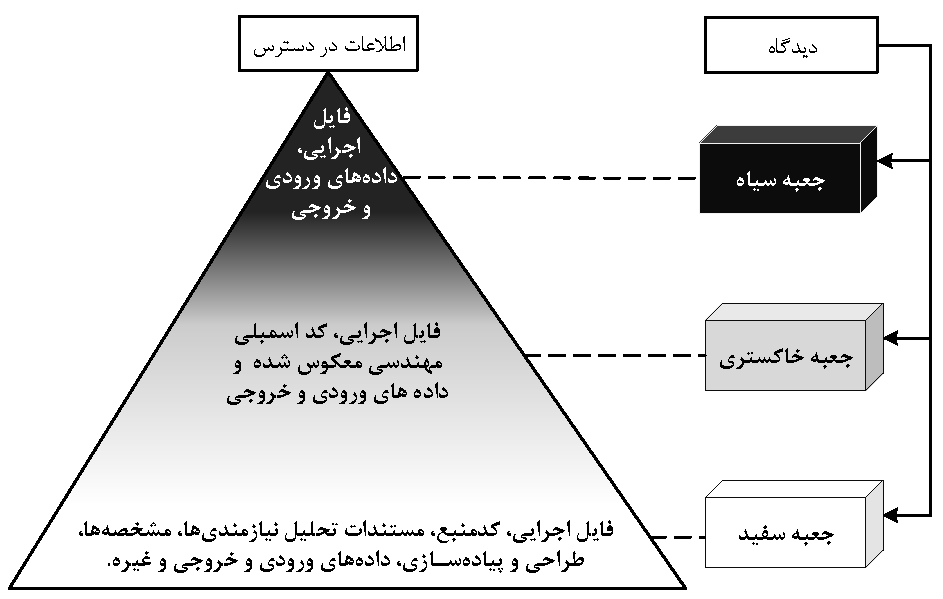
\includegraphics[width=\textwidth, clip=true,  trim= 0 0 0 0]{chapter2/ch2_box_veiw_test_triangle_crop.pdf}
  	%\includegraphics[width=\textwidth]{figs/chapter1/ch1_fuzz_testing_flowchart2.png}
  	\caption[دیدگاه جعبه در آزمون نرم‌افزار]
  	{
  		طرح‌واره‌ای از دیدگاه جعبه بر اساس اطلاعات در دسترس به‌صورت یک مثلث آزمون\cite{ZakeriSeminar2017}.
  	}
  	\label{ch2_box_veiw_test_triangle_crop.pdf}
  \end{figure}
  
  
  همان‌طور که در این طرح‌واره پیداست، در رأس مثلث، هیچ اطلاعی از ساختار داخلی \gls{SUT} در اختیار آزمون‌گر نیست. در واقع با برنامه به مثابه یک جعبه سیاه که ورودی را دریافت و خروجی تولید می‌کند، رفتار می‌شود. این نوع آزمون معمولاً روی برنامه‌هایی که منتشر شده‌اند و توسط افرادی خارج از تیم توسعه و پشتیبانی محصول انجام می‌شود. هدف آن هم بیشتر کشف آسیب‌پذیری‌‌ها و ضعف‌های امنیتی است. در پایین مثلث، دیدگاه جعبه سفید وجود دارد. در اینجا تقریباً تمامی اطلاعات \gls{SUT} در دسترس است. دیدگاه جعبه خاکستری مابین دو دیدگاه قبلی قرار دارد. در این دیدگاه از فنون مهندسی معکوس برای استخراج اطلاعات از \gls{SUT} استفاده می‌شود. هریک از این دیدگاه‌ها مزایا و معایب خاص خود را دارند\cite{Khan2012}. آزمون فازی هم که در ادامه مطرح می‌شود، قابل تقسیم به‌این سه دسته است. آزمون فازی جعبه خاکستری، برای مثال، بسیار ثمربخش بوده است   \cite{DBLP:journals/corr/abs-1711-04596, Zalewsky2013}. روش پیشنهادی در این پایان‌نامه برای تولید داده آزمون، قابل استفاده در هر سه دسته آزمون فازی است. برای ارزیابی روش پیشنهادی در این پایان‌نامه، در \hyperref[ch:5]{فصـل 5}، اما از آزمون جعبه سفید، استفاده کرده‌ایم تا بتوانیم معیارهای پوشش کد و بخش‌های اجرا شده را به‌دقت اندازه‌گیری نماییم. از طرفی \lr{SUT} انتخابی ما متن باز و رایگان بوده و در این حالت کد منبع آن دردسترس است. 
 
     
  \subsection{اندازه‌گیری پوشش کد}\label{sec:instrumenting}
   هدف از مطرح کردن دیدگاه جعبه در بخش \ref{box_view}، اشاره به امکانات لازم برای اندازه‌گیری معیارهای پوشش از جمله پوشش کد بود. در آزمون جعبه سفید که کد منبع برنامه وجود دارد، مشاهده پوشش کد برنامه با اضافه کردن دستوراتی به متن کد به آسانی امکان پذیر است. این عمل را \gls{Instrumenting} کد یا تجهیز برنامه به کد رهگیری می‌نامند\cite{Rathaus:2007:OSF:1536880}. در محیط \lr{GNU/GCC} (زبان‌های \lr{C} و \lr{C++})، برای \gls{Instrumenting} کافی است کد منبع برنامه را همراه با پرچم‌های
   \lr{\texttt{-fprofile-arcs}}
   و
   \lr{\texttt{-ftest-coverage}}
   کامپایل کنیم:\\
   
   
   \begin{LTR}
   	\begin{lstlisting}[language=bash, caption={\rl{ابزارگذاری کد در محیط \lr{GNU/GCC}.}}, label={codesnip2}]
   	~$ gcc -g -fprofile-arcs -ftest-coverage -o test test.c
   	~$ ./test f1 f2
   	~$ gcov test.c
   	~$ more test.c.gcov\end{lstlisting}
   \end{LTR}
سطر اول برنامه \ref{codesnip2} برنامه \lr{test} را با پرچم‌های ذکر شده کامپایل می‌کند. سطر دوم برنامه را با دو آرگومان خط فرمان \texttt{f1} و \texttt{f2} اجرا می‌کند. سطر سوم پوشش کد اجرای اخیر برنامه را محاسبه و فایلی تحت عنوان \texttt{ test.c.gcov} تولید می‌کند. در سطر چهارم این فایل برای مشاهده باز می‌شود. افزون بر این، پرچم‌هایی برای اخذ انواع سطوح پوشش کدی که بحث شد، از جمله پوشش شاخه، وجود دارد \cite{Rathaus:2007:OSF:1536880}. 

  محیط ویژوال استادیو ابزار \lr{vsinstr} را برای ابزارگذاری کد برنامه و \lr{VSPerfMon} را برای اندازه‌گیری پوشش کدِ زبان‌های پشتیبانی شده توسط این محیط، ارائه می‌دهد که البته در حضور کد منبع برنامه قابل استفاده هستند. هنگامی که کد منبع در اختیار نباشد کار اندکی دشوار می‌شود. در این موارد، بایستی از ابزارهای مهندسی معکوس و ابزارگذاری کد باینری استفاده کرد.
 \lr{DynamoRIO}\LTRfootnote{\href{http://www.dynamorio.org/}{http://www.dynamorio.org/}}\cite{Bruening:2004:ETC:1087758}،
 \lr{Pin}\LTRfootnote{\href{https://software.intel.com/en-us/articles/pin-a-dynamic-binary-instrumentation-tool}{https://software.intel.com/en-us/articles/pin-a-dynamic-binary-instrumentation-tool}}\cite{Luk:2005:PBC:1064978.1065034}،
 \lr{PaiMei}\LTRfootnote{\href{https://github.com/OpenRCE/paimei}{https://github.com/OpenRCE/paimei}}\cite{Rathaus:2007:OSF:1536880}
  و 
  \lr{QEMU}\LTRfootnote{\href{https://www.qemu.org/}{https://www.qemu.org/}} \cite{QEMU2018}
 ابزارهایی برای این منظور فراهم کرده‌اند.


  
\section{آزمون فازی}
\gls{FuzzTesting}\cite{Miller:1990:ESR:96267.96279,Miller1995,Forrester:2000:ESR:1267102.1267108,Miller:2006:ESR:1145735.1145743}
همان‌طورکه قبلاً هم گفتیم، فرایند ساده تولید و سپس تزریق یک ورودی ناخواسته (بدشکل شده یا نامتعارف) به \gls{SUT} است. چنان‌چه برنامه بر اثر پردازش این ورودی ناخواسته دچار خرابی شود، حافظه برنامه مورد تحلیل قرار گرفته و خطای احتمالی موجود در کد آشکار می‌گردد. به دلیل اینکه \gls{SUT} هنگام آزمون اجرا می‌شود، آزمون فازی، نوعی آزمون پویا است. چون \gls{SUT} با تعداد ورودی‌های بسیار زیادی مورد آزمون قرار می‌گیرد، آزمون فازی را می‌توان نوعی\gls{StressTesting} هم به‌شمار آورد. فرایند معمول آزمون فازی در ‏شکل
\ref{ch2_fuzz_testing_flowchart_crop.pdf} نشان داده شده است.


%% Need to crop all figures
%% https://pdfresizer.com/
%%
\begin{figure}%[tbh!]%[ht]%[t!]
	\centering
	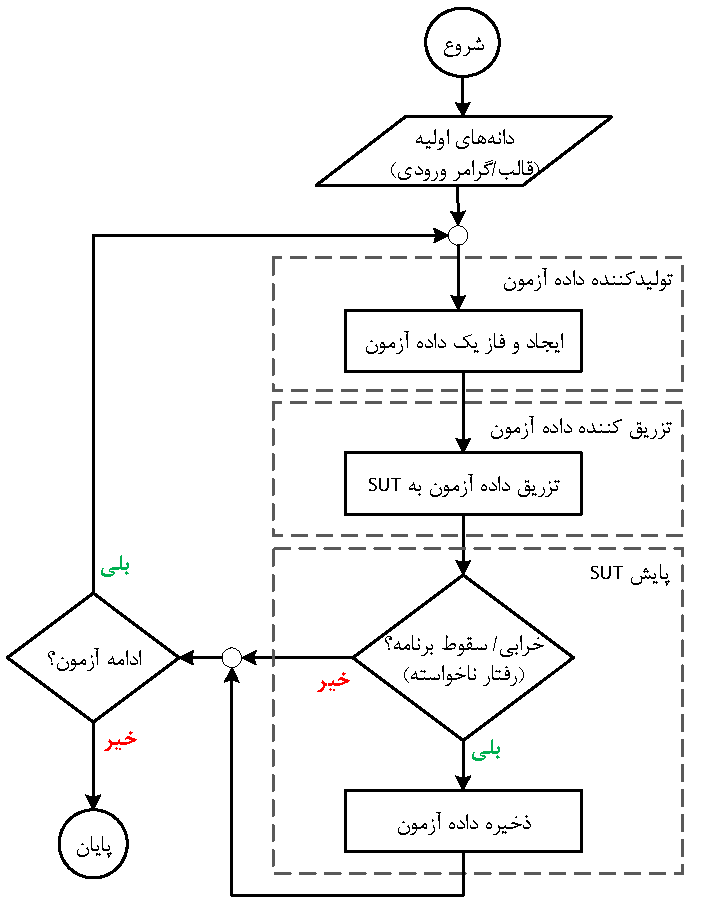
\includegraphics[width=0.9\textwidth, clip=true,  trim= 0 0 0 0]{chapter2/ch2_fuzz_testing_flowchart_crop.pdf}
	%\includegraphics[width=\textwidth]{figs/chapter1/ch1_fuzz_testing_flowchart2.png}
	\caption[روندنمای  فرایند آزمون فازی]
	{
		روندنمای فرایند آزمون فازی در حالت ساده که با اقتباس از مراجع مختلف ترسیم شده است. پیمانه‌های مورد نیاز برای خودکارسازی فرایند با مستطیل خطچین مشخص شده‌اند. شرایط ادامه آزمون می‌تواند بر عهده فرد آزمون‌گر قرار داده شود یا توسط خود فازر تعیین گردد.
	}
	\label{ch2_fuzz_testing_flowchart_crop.pdf}
\end{figure}



\subsection{فازر}\label{sec:fuzzer}
\gls{Fuzzer} ابزاری است که فرایند آزمون فازی را خودکار می‌کند. پیاده‌سازی هریک از \gls{Module}‌های شکل
\ref{ch2_fuzz_testing_flowchart_crop.pdf}
و تجمیع آنها در کنار یکدیگر یک \gls{Fuzzer} را ایجاد می‌کند. تمرکز اصلی در یک \gls{Fuzzer}، نحوه تولید ورودی جدید به عنوان داده آزمون است به‌گونه‌ای که می‌توان آن را وجه تمایز اصلی فازرهای مختلف دانست. روش‌های تولید داده در فازرها قابل تفکیک به دو دسته کلی روش‌های \gls{MutationBased} یا جهش و روش‌های \gls{GenerationBased} 
هستند \cite{Chen2018}.


در روش \gls{MutationBased}، تعداد یک یا بیشتر داده ورودی \gls{Valid} به‌عنوان \gls{InitialSeed} برای تولید داده‌های آزمون بیشتر به‌کار می‌رود.  \gls{InitialSeed} جهش (تغییر ناگهانی) می‌یابد تا داده آزمون دیگری تولید شود. جهش می‌تواند ساده باشد؛ شبیه معکوس کردن یک بیت، جایگزین کردن یک کاراکتر، یا پیچیده‌تر باشد؛ شبیه شناسایی و تکرار ساختارهای مشخص در داده، جایگزینی اعداد صحیح و حقیقی با مقادیر مرزی (بسیار بزرگ یا کوچک) و غیره. ساختن یک فازر مبتنی بر جابه‌جایی و تولید ورودی بد شکل و مخرب با آن، آسان است و نیاز به شناخت قبلی ساختار داده ورودی مورد جهش ندارد. عیب روش مبتنی بر جابه‌جایی اینجاست که این روش وابسته به تنوع ورودی‌های نمونه است. بدون وجود ورودی‌های مختلف با پیچیدگی کافی، این نوع فارز‌ به پوشش کد بالایی دست نمی‌یابد \cite{Kettunen2014}. به عبارت دیگر دانه اولیه در فازر مبتنی بر جابه‌جایی بسیار حائز اهمیت است.
 \lr{AFL}\LTRfootnote{American Fuzzy Lop (\href{http://lcamtuf.coredump.cx/afl/}{http://lcamtuf.coredump.cx/afl/})}\cite{Zalewsky2013}، \lr{FileFuzz}\LTRfootnote{\href{http://www.fuzzing.org/}{http://www.fuzzing.org/}}\cite{Sutton:2007:FBF:1324770}
 و
  \lr{Radamsa}\LTRfootnote{\href{https://gitlab.com/akihe/radamsa}{https://gitlab.com/akihe/radamsa}}\cite{Kettunen2014}
 نمونه‌هایی از فــازرهای مبتنی بر جابه‌جایی هستند.
 
 
 روش مبتنی بر تولید، داده‌های آزمون را به‌صورت کاملاً تصادفی یا از روی یک توصیف صوری مانند گرامر، قالب، یا مدل تولید می‌کند. در حالت دوم، از مشخصه‌های داده ورودی، برای ساخت یک \gls{GenerativeModel} استفاده می‌شود. این روش بیشتر روی قالب‌های داده‌ای که مستنداتی از مشخه‌های آنها در دسترس است، به‌کار می‌رود که در مقایسه با فازرهای مبتنی بر جابه‌جایی، معمولاً به پوشش کد بالاتری دست می‌یابد. با این حال، همان‌طور که در فصل 1 هم اشاره شد، زمان و هزینه زیادی باید صرف شود تا مشخصه‌های یک قالب داده، کامل فهمیده و مدل خوبی از آن تهیه شود؛ زیرا، این کار تمام خودکار نیست \cite{Miller2007} و از طرفی، مستندات ساختار ورودی همواره در دسترس آزمون‌گر، نیستند.
 SPIKEfile\LTRfootnote{\href{http://fuzzing.org/}{http://fuzzing.org/}}\cite{Sutton:2007:FBF:1324770} و
 Peach\LTRfootnote{\href{https://www.peach.tech/}{https://www.peach.tech/}}
 نمونه‌ای از فازرهای مبتنی بر تولید هستند. روش‌های ترکیبی نیز وجود دارد که از ویژگی‌های هر دو روش بیان شده در تولید مورد آزمون کمک می‌گیرد. یک مثال از فازرهای ترکیبی LangFuzz \cite{Holler2012} است.
 
 
 \subsection{معماری فازرها}\label{sec:fuzzers_architechture}
 یک معماری مرجع برای فازرها وجود ندارد؛ ولی می‌توان از روی فرایند ترسیم شده برای آزمون فازی (شکل  \ref{ch2_fuzz_testing_flowchart_crop.pdf})، پیمانه‌های اصلی لازم برای یک فازر را پیشنهاد کرد. پیمانه اول تولید کننده \gls{TestData}است که داده‌های ورودی لازم برای آزمون را تولید می‌کند. دیدیم که روش‌های مختلفی برای تولید داده آزمون وجود دارند. پیمانه دوم تزریق کننده داده آزمون است که وظیفه آن تحویل داده‌های تولید شده توسط تولیدکننده به \gls{SUT} است. هر برنامه واسط مختص به خود را دارد. واسط می‌تواند \gls{CLI}، گرافیکی (\gls{GUI})، پروتکل شبکه یا فایل باشد. هدف این پایان‌نامه برنامه‌هایی هستند که ورودی آنها فایل است. معمولاً داده‌های ورودی به‌شکل فایل (مثل \gls{PDF}) ساختار پیچیده‌تری نسبت به داده‌های \gls{CLI} و پروتکل‌های شبکه دارند و تولید آنها سخت‌تر است. فازری که برای آزمون این برنامه‌ها توسعه داده می‌شود، \gls{FileFormatFuzzer} هم نامیده می‌شود \cite{Sutton:2007:FBF:1324770}.
 
 
 آخرین پیمانه مورد نیاز ابزار یا محیط پایش است که \gls{SUT} را پایش می‌کند تا در صورت بروز خرابی ضمن ذخیره حالت برنامه، محل وقوع خرابی را بتواند با تحلیل حافظه برنامه مشخص کند. البته ابزارهای مستقل زیادی برای این منظور وجود دارند که می‌توان از آنها بهره گرفت. 
 \lr{Application Verifier}\LTRfootnote{\href{https://docs.microsoft.com/en-us/windows-hardware/drivers/debugger/application-verifier}{https://docs.microsoft.com/en-us/windows-hardware/drivers/debugger/application-verifier}}
 \cite{ApplicationVerifier}
 یک ابزار پایشِ قابل استفاده در سیستم عامل ویندوز است. ممکن است فازر، یک بازخورد از ابزار پایش برای تولید داده آزمون بعدی دریافت کند. این بازخورد عموماً حاوی اطلاعات مربوط به پوشش کد اجرای برنامه است. بر این اساس فازرها به دو دسته دارای حلقه بازخورد و بدون حلقه بازخورد تقسیم‌بندی می‌شوند \cite{Chen2018}.
 AFL\cite{Zalewsky2013}
 یک فازر دارای حلقه بازخورد است. در این پایان‌نامه یک فازر ساده قالب فایل بدون حلقه بازخورد ارائه می‌دهیم. تمرکز برروی نحوه تولید داده آزمون به روش \gls{GenerationBased} / گرامر است.
 
 
 
 \subsection{آسیب‌پذیری}
 آزمون فازی می‌تواند برای اهداف مختلفی استفاده شود، اما مهمترین هدف آن تحلیل نرم‌افزار به منظور کشف آسیب‌پذیری‌ها است. یعنی می‌توان آن را نوعی \gls{PenetrationTesting}، \gls{RobustnessTesting} و \gls{SecurityTesting} هم تعریف کرد. تعاریف گوناگونی برای اصطلاح آسیب‌پذیری نرم‌افزار وجود دارد. آسیب‌پذیری را می‌توان اجتماع سه عنــصر دانست: وجود یک خطا در نرم‌افزار، دسترسی مهاجم به خطا و قابلیت مهاجم برای \gls{Exploit} از خطا \cite{Chen2018,InternetSecurityGlossary}. چنانچه پیش از این اشاره شد، خطا، نرم‌افزار را در یک حالت اشکال قرار می‌دهد که منجربه خرابی می‌شود. بعضی خطاها ممکن است تنها منجربه خرابی نرم‌افزار و بروز رفتار ناخواسته (مغایر با مشخصه‌ها) شوند. بنابراین صرف وجود یک خطا در نرم‌افزار آسیب‌پذیری محسوب نمی‌گردد 
 \cite{Sutton:2007:FBF:1324770,Rathaus:2007:OSF:1536880}.
 
 
 انواع مختلفی از خطاها وجود دارند که می‌توانند توسط فازرها کشف شوند؛ به‌ویژه آنهایی که از جنس نقض دسترسی به حافظه هستند. خطاهای فساد حافظه بدون شک رایج‌ترین و مؤثرترین روش بهره‌برداری خرابکارانه از یک سیستم کامپیوتری محلی یا راه دور هستند. اگر حافظه بتواند به روشی خراب شود (یک آدرس بازگشت، یک اشاره‌گر پشته، یک اشاره‌گر تابع و غیره) اغلب اجرا می‌تواند به کد تهیه شده توسط مهاجم هدایت شود. بیشترین آسیب‌پذیری‌هایی که معمولاً توسط محققین حوزه امنیت کشف می‌شوند، مرتبط با \gls{Buffer} (یک ناحیه ثابت از حافظه اصلی در اختیار برنامه) هستند؛ از جمله سرریز میانگیر، سرریز پشته، سرریز عدد صحیح و غیره \cite{Takanen:2008:FSS:1404500}. در آزمون فازی به‌دنبال یافتن چنین خطاهایی از طریق تزریق ورودی بدشکل و خرابی حافظه \gls{SUT} هستیم. مطالعه و طبقه‌بندی کاملی از انواع آسیب‌پذیری‌ها در \cite{ZakeriSeminar2017} انجام شده است.  
 
 
 
 
 %%%%%%%%%%%%%%%%%%%%%%%%%%%%%%%
 %%%  Deep Learning Section  %%%
 %%%%%%%%%%%%%%%%%%%%%%%%%%%%%%%
 
 \section{یادگـیری ژرف}
  \gls{DeepLearning}
مجموعه‌ای از فنون یادگیری ماشینی است که در آن بردار ویژگی‌ها به‌صورت خودکار از داده‌های خام استخراج می‌گردد. ابزار اصلی و غالب در این فنون از یادگیری،  \glspl{NeuralNetwork} هستند. در حالت ساده \glspl{NeuralNetwork} به مسئله یک تابع را نسبت داده و آن را مدل می‌کند. پارامترهای این تابع سپس در فرایند آموزش مدل، تخمین زده می‌شوند. در \gls{DeepLearning} تعداد این پارامترها صدها، هزارها و گاهی میلیون‌ها برابر افزایش می‌یابد که در نتیجه قدرت  \gls{Representation} و حل مسئله مدل، افزایش خواهد یافت. شبکه عصبی در این حالت یک گراف با ژرفای بیش از یک یال، خواهد بود که به آن \gls{DeepNeuralNetwork} هم می‌گویند. شبکه عصبی ژرف بدین ترتیب قادر به استخراج و تمییز جزئی‌ترین ویژگی‌های مسئله و در نتیجه بهبود دقت حاصله، خواهد بود \cite{Goodfellow-et-al-2016}.
 
 
 وجود تعداد بسیاری پارامتر در مدل‌های یادگیری ژرف، سبب می‌شود که آموزش این مدل‌ها از لحاظ محاسباتی سنگین و زمان‌بر باشد. بسیاری از موانع تئوری و عملی آموزش این مدل‌ها به‌تازگی رفع شده‌اند. برای مسائل مختلف، مدل‌های متفاوتی با شبکه‌های عصبی ژرف طراحی و ساخته می‌شوند. \gls{FeedforwardNeuralNetwork} ساده‌ترین نوع است. شبکه عصبی پیچشی (\gls{CNN}) مناسب وظایف بینایی ماشین و شبکه عصبی مکرر (\gls{RNN}) مناسب وظایف پردازش زبان طبیعی (\gls{NLP}) (وظایف مبتنی بر \gls{Sequence}) ایجاد شده‌اند. وجه مشترک همه شبکه‌های نام‌برده، بلوک سازنده آن یعنی \gls{Neuron} است \cite{Jurafsky2017}. 
 
 
 
 \subsection{عصب}
 بلوک محاسباتی پایه در بستر شبکه‌های عصبی، \gls{Neuron} یا \gls{Unit} است. یک عصب تعدادی عدد حقیقی را به‌عنوان ورودی گرفته، محاسباتی روی آنها انجام داده و یک خروجی تولید می‌کند. محاسبه بدین صورت است که عصب جمع وزن‌دار ورودی‌هایی که به آن وارد می‌شوند را به همراه یک مقدار اضافی به عنوان \gls{Bias} حساب می‌کند. سپس برای جلوگیری از محدود شدن فضای توابع قابل تخمین به فضایی خطی، یک تابع غیرخطی، موسوم به \gls{ActivationFunction} (تابع فعّالیت)، روی حاصل جمع اعمال می‌شود. توابع انگیزش متداول عبارتند از \lr{sigmoid} و \lr{tanh}. شکل \ref{ch2_single_neuron_internal_structure_crop.pdf} ساختمان داخلی یک عصب تنها با ورودی‌های $x_1 $، $ x_2 $ و $ x_3 $، متقابلاً وزن‌های $ w_1 $، $ w_2 $ و $ w_3 $ و مقدار بایاس $ b $ را نشان می‌دهد. محاسبات این عصب مطابق رابطه‌های \ref{NeuronActivation} و \ref{NeuronActivation2} است.
 \begin{equation}\label{NeuronActivation}
 z = b+ \sum_iw_ix_i 
 \end{equation}
 \begin{equation}\label{NeuronActivation2}
 y = \sigma(z)
 \end{equation}
 
 
 رابطه \ref{NeuronActivation} را می‌توان به صورت ضرب داخلی بردارهای $ W $ و $ x $ هم نشان داد که نمایش مرسوم‌تری است \cite{Jurafsky2017}:
  \begin{equation}\label{NeuronActivation3}
 z = b+ W.x
 \end{equation} 
 
 
 \begin{figure}%[ht!]%[tbh!]%[ht]%[t!]
 	\centering
 	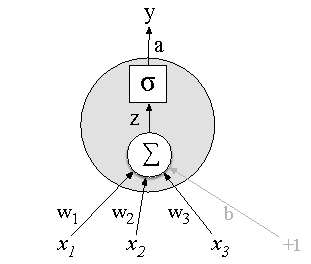
\includegraphics[width=0.5\textwidth, clip=true,  trim= 0 0 0 0]{chapter2/ch2_single_neuron_internal_structure_crop.pdf}
 	%\includegraphics[width=\textwidth]{figs/chapter1/ch1_fuzz_testing_flowchart2.png}
 	\caption[ساختمان داخلی یک عصب]
 	{
 		ساختمان داخلی یک عصب با ورودی‌های $x_1 $، $ x_2 $ و $ x_3 $، به‌ترتیب با وزن‌های $ w_1 $، $ w_2 $ و $ w_3 $، مقدار بایاس $ b $ و خروجی $y$ \cite{Jurafsky2017}.
 	}
 	\label{ch2_single_neuron_internal_structure_crop.pdf}
 	%\ref{ch2_single_neuron_internal_structure_crop.pdf}
 \end{figure}
 
 
 
 \subsection{شبکه عصبی روبه‌جلو}
 شبکه روبه‌جلو را می‌توان با یک گراف جهت‌دار بدون دور (\gls{DAG}) نشان‌ داد. هر گره یک عصب را نشان می‌دهد. گره‌هایی که مسیری به یکدیگر ندارند، یک لایه را تشکیل می‌دهند. ورودی هر لایه، خروجی عصب‌های لایه قبلی است. هر لایه بازنمایی یک \gls{Concept} در قالب یک تابع است و مسئله ترکیبی از این \glspl{Concept} است. یک شبکه با دو لایه تابع 
 $ f(x)=W_2\sigma(W_1 x) $
 را پیاده می‌کند که $ W_1 $ و $ W_2 $  ماتریس پارامترهای تابع و $ \sigma $ تابع انگیزش است.
 $ f(x)=W_3\sigma(W_2\sigma(W_1 x)) $
 معرف یک شبکه سه‌لایه خواهد بود. شکل \ref{ch2_feed_forward_neural_network_crop.pdf} دو گراف محاسباتی با ژرفای 2 و 3 لایه (به ترتیب از چپ به راست) را نشان می‌دهد. لایه‌های میانی را \glspl{HiddenLayer} هم می‌گویند. توجه شود که ورودی اول شبکه یک لایه محاسباتی نیست و بنابراین در شمارش لایه‌ها، شمرده نمی‌شود.
 
 
     
 \begin{figure}[ht!]%[tbh!]%[ht]%[t!]
 	\centering
 	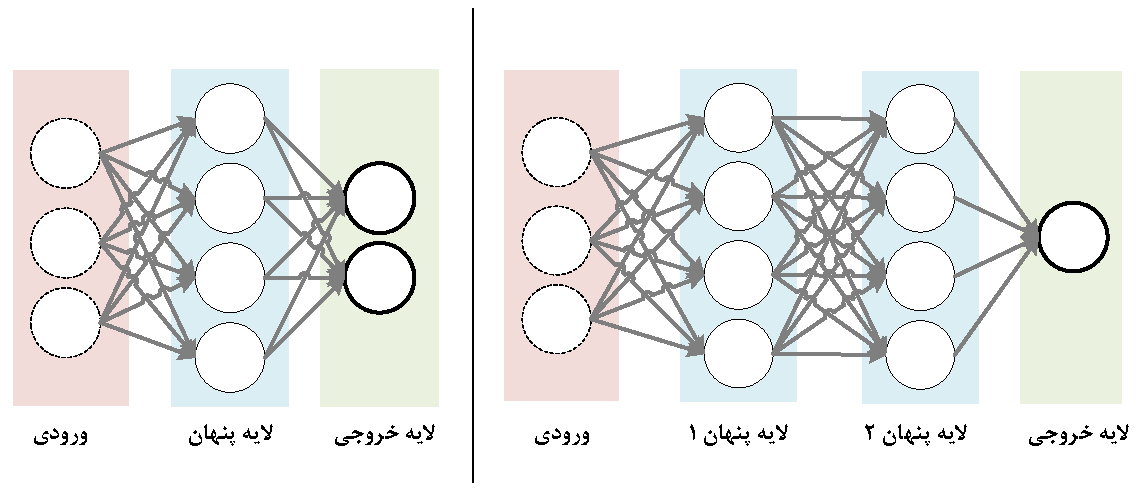
\includegraphics[width=\textwidth, clip=true,  trim= 0 0 0 0]{chapter2/ch2_feed_forward_neural_network_crop.pdf}
 	%\includegraphics[width=\textwidth]{figs/chapter1/ch1_fuzz_testing_flowchart2.png}
 	\caption[گراف محاسباتی شبکه عصبی روبه‌جلو]
 	{
 		گراف محاسباتی برای دو شبکه عصبی روبه‌جلوی فرضی. چپ: یک شبکه عصبی دو لایه (یک لایه پنهان متشکل از چهار عصب و یک لایه خروجی متشکل از دو عصب) به‌همراه سه ورودی. راست: یک شبکه عصبی سه‌لایه (دو لایه پنهان هر کدام متشکل از چهار عصب و یک لایه خروجی متشکل از یک عصب) و به‌همراه سه ورودی. 
 	}
 	\label{ch2_feed_forward_neural_network_crop.pdf}
 	%\ref{ch2_feed_forward_neural_network_crop.pdf}
 \end{figure}
 
 
 \subsection{آموزش شبکه روبه‌جلو}\label{feedforwardtraining}
 هدف از آموزش شبکه، تعیین مقادیر مناسب برای ضرایب و بایاس‌ها و سپس استفاده از شبکه برای انجام \gls{Task} مورد نظر است. داده‌هایی که در فرایند آموزش شبکه استفاده می‌گردد \gls{TrainingSet} نامیده می‌شوند. داده‌هایی که شبکه با آن مورد سنجش قرار می‌گیرد، \gls{TestSet} نامیده می‌شوند و مجموعه سوم از داده‌ها که در طول فرایند آموزش شبکه برای انتخاب بهترین راهکارهای یادگیری به‌کار گرفته می‌شوند، به نام \gls{ValidationSet} شناخته می‌شوند \cite{Goodfellow-et-al-2016}. 
 
 
 شبکه عصبی در یک راهبرد \gls{Supervised} آموزش می‌بیند. در \gls{SupervisedLearning} هر نمونه در مجموعه داده، علاوه بر بردار ویژگی‌ها با یک \gls{Label} همراه است که نقش ناظر را ایفا می‌کند. \gls{Classification} نمونه‌ای از وظایف \gls{SupervisedLearning} است. در این وظیفه برای هر ورودی، کلاس خروجی آن در زمان آموزش مشخص است.
 
 
 در فرایند آموزش ابتدا پارامترهای شبکه مقداردهی اولیه می‌شوند (معمولاً به‌صورت تصادفی). سپس به ازای هر ورودی از مجموعه آموزش، عصب‌های هر لایه خروجی خود را تولید می‌کنند تا زمانی که خروجی نهایی شبکه تولید شود. این مرحله را \gls{ForwardPass} می‌گویند. از آنجایی که خروجی درست برای ورودی مربوطه در زمان آموزش دردسترس است (\gls{SupervisedLearning})؛ اختلاف مقدار محاسبه شده توسط شبکه ($ \hat{y} $) و مقدار واقعی ($ y $)، توسط تابعی موسوم به \gls{ErrorFunction} یا \gls{CostFunction} یا تابع هدف محاسبه می‌شود \cite{Karpathy2016}. توابع مختلفی برای این منظور می‌توان تعریف کرد. 
 تابع \gls{MeanAbsoluteError} (رابطه \ref{MAELossFunction})، تابع \gls{MeanSquaredError} (رابطه \ref{MSELossFunction}) و تابع \gls{CrossEntropyError} (رابطه \ref{CrossEntropyLossFunction}) توابعی هستند که بسته به وظیفه مورد نظر استفاده می‌شوند \cite{Sautermeister2016}.
\begin{equation}\label{MAELossFunction}
	L_{MAE}(\hat{y}, y; W,b)=\frac{1}{n}\sum_{i=1}^{n}|\hat{y_{i}}-y_{i}|
\end{equation}
\begin{equation}\label{MSELossFunction}
L_{MSE}(\hat{y}, y; W,b)=\frac{1}{n}\sum_{i=1}^{n}(\hat{y_{i}}-y_{i})^2
\end{equation}
\begin{equation}\label{CrossEntropyLossFunction}
L_{CE}(\hat{y}, y; W,b)=-\sum_{i=1}^{n}y_i\log{\hat{y_{i}}}
\end{equation}
 
 در روابط \ref{MAELossFunction} تا \ref{CrossEntropyLossFunction}، $ n $ تعداد نمونه‌ها یا تعداد مشاهده‌ها است. در این پایان‌نامه از تابع \gls{CrossEntropyError} استفاده می‌کنیم که برای وظیفه‌های طبقه‌بندی با بیش از دو کلاس مناسب‌ است \cite{Karpathy2016}. وقتی میزان خطا در گذرجلو مشخص شد، هدف تغییر میزان پارامترهای شبکه به‌نحوی است که خطا کمینه شود (رابطه \ref{argminloss}):
 \begin{equation}\label{argminloss}
 	f^{*} = arg \min_{W,b} L(\hat{y}, y; W,b)
 \end{equation}
که $ f^{*} $ تابع یادگیری شده و مقادیر $ W $ و $ b $ پارامترهای شبکه هستند. سایر مقادیر را که در طول این فرایند یادگیری نمی شوند، \gls{Hyperparameter} می‌نامند. از جمله ابر پارامترها می‌توان به تعداد لایه‌ها و تعداد عصب‌ها در هر لایه اشاره کرد، که از آنها برای تعیین اندازه شبکه استفاده می‌‌گردد.
 
 برای کمینه‌سازی خطا، مشتقات جزئی تابع خطا نسبت به هریک از پارامترها در لایه خروجی محاسبه می‌شود (گرادیان) و سپس این روند از طریق روال \gls{Backpropagation} تا ابتدای شبکه پیش‌ می‌رود و مقدار هر پارامتر درسوی کاهش گرادیان با ضریبی موسوم به \gls{LearningRate} بروزرسانی می‌شود. \gls{LearningRate} عدد کوچکی (در مقیاس صدم و هزارم) در نظر گرفته می‌شود که برای همگرایی آهسته و پیوسته شبکه و جلوگیری از واگرا شدن آن لازم است. \gls{LearningRate} یکی دیگر از \gls{Hyperparameter}های مورد نیاز آموزش شبکه‌های ژرف است. الگوریتم \gls{Backpropagation} در واقع یک کاربرد بازگشتی از قاعده مشتق زنجیری در حساب دیفرانسیل است \cite{Karpathy2016}. در اینجا به بیان جزئیات الگوریتم‌های بهینه‌سازی نمی‌پردازیم؛ چارچوب‌های یادگیری ژرف انواع مختلفی از این الگوریتم‌ها را پیاده‌سازی و در اختیار قرار داده‌اند. توضیحات کاملی از این الگوریتم‌ها در  \cite{Goodfellow-et-al-2016} آمده است.
 
 
 \subsubsection{شرایط توقف آموزش}\label{sec:stop_conditions}
 فرایند آموزش شبکه می‌تواند تا بی‌نهایت ادامه داشته باشد. بنابراین بایستی یک قانون برای توقف آن تعریف شود. گزینه‌‌های زیادی وجود دارد که تحت چه شرایطی آموزش را خاتمه دهیم. همچنین ترکیب این شرایط نیز امکان‌پذیر است. برخی از این شرایط عبارتند از \cite{Sautermeister2016}:
 
 \begin{enumerate}
 	\item{
 	هنگامی که تعداد مشخصی \gls{Epoch} طی شود (هر \gls{Epoch} برابر تعداد تکرارهایی است که برای مرور کل مجموعه آموزش لازم است).
 	} 
 	\item{
 	هنگامی که خطای مجموعه ارزیابی (برای تعداد مشخصی \gls{Epoch} متوالی) کاهش پیدا نکند.
 }

\item{
	هنگامی که تغییرات میزان خطا (برای تعداد مشخصی \gls{Epoch} متوالی) کمتر از یک حد آستانه شود.
} 
\item{
	هنگامی که یک زمان مشخص از فرایند آموزش سپری شود.
} 
\end{enumerate} 



 \subsubsection{منظم‌سازی}
مشکل رایجی که هنگام آموزش شبکه عصبی باید جلوگیری شود اثر \gls{Overfitting} است. \gls{Overfitting} یعنی با کاهش خطا روی مجموعه آموزش، خطای مجموعه‌‌های ارزیابی و آزمون به‌طور ناگهانی افزایش ‌یابد \cite{Goodfellow-et-al-2016}. یک دلیل می‌تواند به‌اندازه کافی بزرگ نبودن اندازه مجموعه آموزش باشد. دلیل دیگر می‌تواند پیچیدگی بسیار بالای مدل باشد. پیچیدگی مدل با تعداد پارامترهای  آن مشخص می‌شود. در پیچیدگی بالا ممکن است مدل، \gls{Noise}های موجود در ورودی‌ها را نیز لحاظ کند و متناسب یا برازنده آن شود. در نتیجه هنگام ارزیابی مدل روی داده‌های \gls{TestSet}، خطا بالا می‌رود \cite{Sautermeister2016}. 

راهکارهای مختلفی برای مقابله با مسئله \gls{Overfitting} مدل پیشنهاد شده است. از این راهکارها تحت عنوان فنون \gls{Regularization} یا تنظیم مدل یاد می‌شود. اغلبِ روش‌‌های شناخته شده، پارامترهای دارای مقادیر بالا را که اثرات نوسانی شدیدی دارند، با تابعی جریمه می‌کنند \cite{Karpathy2016}. روش دیگر برای منظم‌سازی 
\lr{Dropout} \cite{JMLR:v15:srivastava14a}
است که بسیار مؤثر و ساده بوده و در مدل‌های یادگیری ژرف معمولاً از آن استفاده می‌شود. در طول آموزش \lr{Dropout} یک عصب را فقط با احتمال $p$ (یک ابر پارامتر) فعال نگه می‌دارد و در غیر این صورت آن را صفر می‌کند. در نتیجه پیچیدگی مدل تنظیم می‌شود.



 
 \subsection{شبکه عصبی مکـرر}
شبکه‌‌های روبه‌جلو در حل مسائلی که ترتیب ورودی در آنها مهم است، مثل ترجمه ماشینی و سایر وظیفه‌های \gls{NLP}، نارسایی دارند. برای مثال در ترجمه ماشینی هر واژه به واژه‌های قبلی خود وابسته است. در این وظیفه‌ها ورودی به‌صورت یک توالی 
$ x = <x^{(1)}, x^{(2)}, x^{(3)}, ..., x^{(n)}> $
است. غالب وظایف حوزه پردازش زبان طبیعی بدین صورت هستند.


شبکه‌های عصبی مکرر
کلاسی از شبکه‌‌های عصبی هستند که به‌صورت یک گراف جهت‌دار دارای دور بیان می‌شوند. به‌عبارت دیگر ورودی هریک از لایه(های) پنهان یا لایه خروجی افزون‌بر خروجی لایه قبل، شامل ورودی‌ای از \gls{TimeStep} قبل به‌صورت بازخورد نیز می‌شود. ‏شکل \ref{ch2_rnn.pdf} یک \gls{RNN} را نشان می‌دهد که در آن لایه پنهان از \glspl{TimeStep} قبلی بازخورد گرفته است. در هر \gls{TimeStep} 
$ t $
 (از
 $ t=1 $ 
 تا 
 $ t=T $)
 یک بردار 
 $ x^{(t)} $
 از توالی ورودی پردازش می‌شود. معادلات گذرجلو شبکه در $ t $ عبارتند از \cite{Goodfellow-et-al-2016}:
 \begin{equation}\label{rnnformula1}
 z^{(t)}=Ux^{(t)}+Wh^{(t-1)}+b
 \end{equation}
 \begin{equation}\label{rnnformula2}
 h^{(t)}=\sigma(z^{(t)})
 \end{equation}
  \begin{equation}\label{rnnformula3}
 y^{(t)} = Vh^{(t)}+c
 \end{equation}
 \begin{equation}\label{rnnformula4}
 \hat{y}^{(t)}=softmax(y^{(t)})
 \end{equation}
 
 
 
 در روابط \ref{rnnformula1} تا \ref{rnnformula4}، $ b $ و $ c $ بایاس و ماتریس‌های  $ U $، $ V $ و $ W $ به‌ترتیب وزن یال‌‌های لایه ورودی به پنهان، پنهان به خروجی و پنهان به پنهان، پارامترهای شبکه هستند. در لایه خروجی به‌جای تابع انگیزش، تابع \gls{Softmax} اعمال می‌شود. این تابع خروجی شبکه را به‌شکل یک توزیع احتمالی معتبر تبدیل می‌نماید و معمولاً در لایه خروجی مدل‌هایی که برای طبقه‌بندی استفاده می‌شوند، قرار می‌گیرد. تابع بیشینه هموار یک بردار $k$تایی از اعداد حقیقی را به عنوان ورودی دریافت نموده و یک بردار $k$تایی از مقادیر حقیقی در بازه  $ [0,1] $ را به عنوان خروجی می‌دهد به‌طوری که جمع مؤلفه‌‌های آن برابر یک خواهد بود (رابطه \ref{softmaxformula}):
 
 \begin{equation}\label{softmaxformula}
 	softmax(x_i) = \frac{e^{x_i}}{\sum_{j=0}^{k}{e^{x_j}}} \quad \textit{\lr{ for i=1 to k}}
 \end{equation}
 
 
 \begin{figure}%[ht!]%[tbh!]%[ht]%[t!]
 	\centering
 	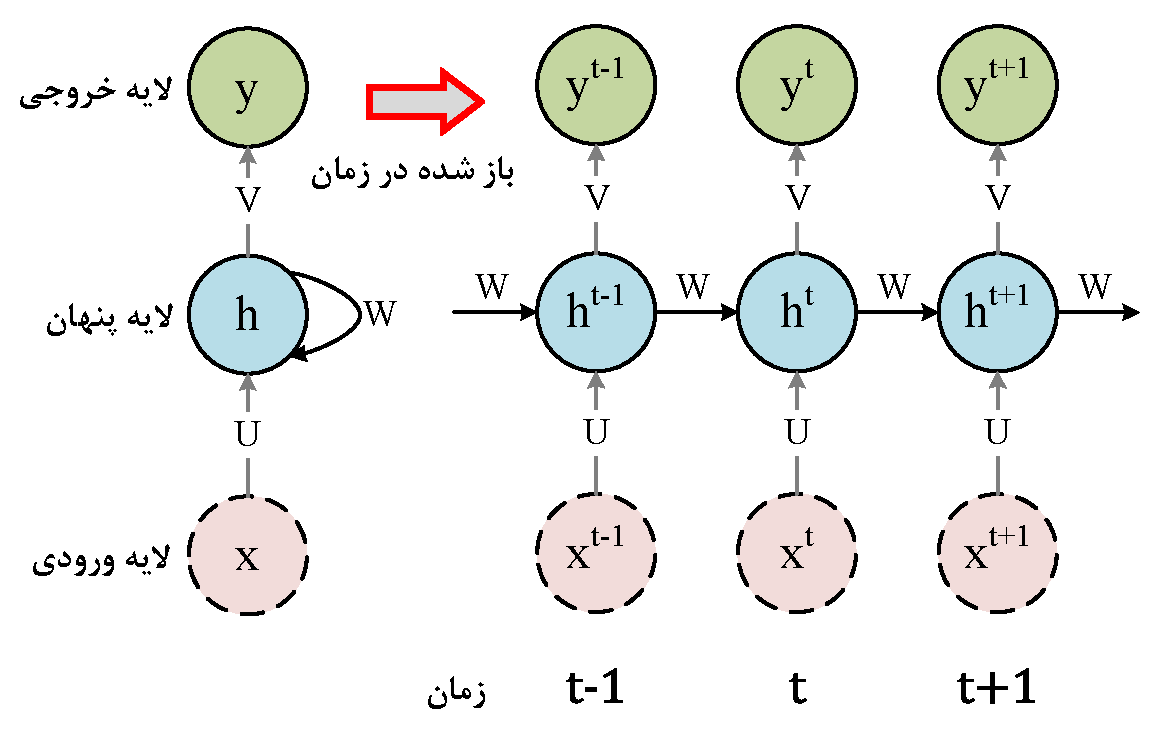
\includegraphics[width=0.8\textwidth, clip=true,  trim= 0 0 0 0]{chapter2/ch2_rnn_crop.pdf}
 	%\includegraphics[width=\textwidth]{figs/chapter1/ch1_fuzz_testing_flowchart2.png}
 	\caption[گراف محاسباتی شبکه عصبی مکرر]
 	{
 		 گراف محاسباتی مربوط به یک شبکه عصبی مکرر با یک لایه پنهان که یک توالی ورودی از مقادیر 
 		 $ x = <x^{(1)}, x^{(2)}, x^{(3)}, ..., x^{(n)}> $
 		 را به یک توالی خروجی از مقادیر 
 		 $ y = <y^{(1)}, y^{(2)}, y^{(3)}, ..., y^{(n)}> $
 		 نگاشت می‌کند. فرض شده است که خروجی $ y $ احتمال‌های نرمال نشده است، بنابراین خروجی نهایی شبکه یعنی $ \hat{y} $ از اعمال تابع بیشینه هموار روی $ y $  حاصل می‌شود. چپ: شبکه عصبی مکرر به‌صورت یال بازگشتی (گراف جهت‌دار دارای دور). راست: همان شبکه به‌صورت باز شده در زمان، به نحوی که هر گره با برچسب مرحله زمانی مشخص شده است \cite{Goodfellow-et-al-2016}.
 	}
 	\label{ch2_rnn.pdf}
 	%\ref{ch2_rnn.pdf}
 \end{figure}
 
 
 
 در ‏شکل \ref{ch2_rnn.pdf}، \gls{RNN} با یک لایه پنهان نشان داده شده است. اما می‌توان \gls{RNN}ژرف با چندین لایه پنهان نیز داشت. همچنین طول توالی‌‌های ورودی و خروجی می‌تواند بسته به مسئله مورد نظر متفاوت باشد. کارپتی\LTRfootnote{A. Karpathy (\href{http://karpathy.github.io/}{http://karpathy.github.io/})}
 	\cite{Karpathy2016}
  \gls{RNN}ها را از منظـر طول توالی ورودی و طول توالی خروجی به چند دسته تقسیم‌بندی کرده است. شکل \ref{ch2_karpathy_rnn_crop.pdf} این دسته‌بندی را نشان می‌دهد.
 
 
 \begin{figure}%[ht!]%[tbh!]%[ht]%[t!]
 	\centering
 	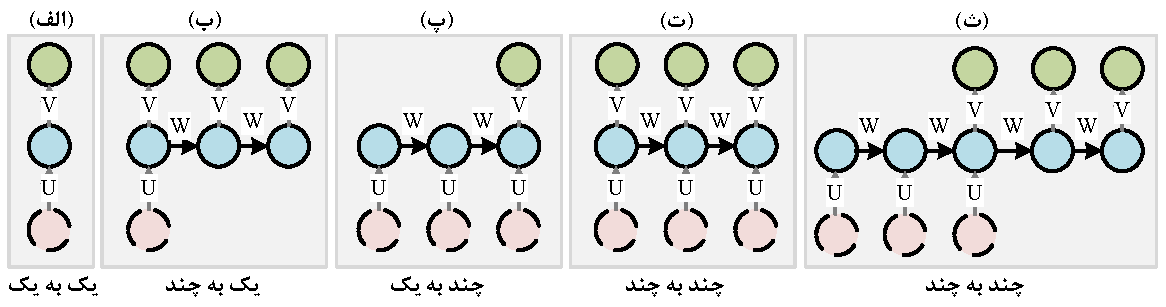
\includegraphics[width=1.0\textwidth, clip=true,  trim= 0 0 0 0]{chapter2/ch2_rnn_karpathy_crop.pdf}
 	%\includegraphics[width=\textwidth]{figs/chapter1/ch1_fuzz_testing_flowchart2.png}
 	\caption[انواع مختلف شبکه عصبی مکرر بر اساس طول توالی ورودی و خروجی]
 	{
 طرح‌واره‌ای از انواع حالت‌های مختلف شبکه عصبی مکرر براساس طول توالی ورودی و طول توالی خروجی. (الف): شبکه عصبی استاندارد، (ب): شبکه یک به چند، (پ): شبکه چند به یک، (ت) و (ث): شبکه‌های چند به چند \cite{Karpathy2016}. 
 	}
 	\label{ch2_karpathy_rnn_crop.pdf}
 	%\ref{ch2_karpathy_rnn_crop.pdf}
 \end{figure}
 
 
 
 \subsubsection{آموزش شبکه عصبی مکرر}
 الگوریتم پس‌انتشار برای آموزش \gls{RNN} هم قابل استفاده است. در واقع \gls{RNN} همان شبکه عصبی روبه‌جلو است که یک بازخورد از وزن‌‌های \gls{TimeStep} قبل دارد. در نتیجه خطا هنوز به‌صورت روی‌به‌عقب از \gls{TimeStep}  $ t $ منتشر می‌شود. بسته به طول توالی ورودی و میزان منابع محاسباتی این انتشار تا \gls{TimeStep}  $ t=1 $ ادامه می‌یابد یا تحت محدودیت تعداد مشخصی \gls{Step} متوقف می‌شود. نسخه‌ای از الگوریتم پس‌انتشار که می‌تواند به‌کل طول توالی ورودی اعمال شود، پس‌انتشار در زمان (\gls{BPTT}) نام دارد. محدودیت منابع محاسباتی ایجاب می‌نماید که طول توالی ورودی مقدار مشخصی قرار داده شود یا پس‌انتشار در تعداد محدودی گام‌زمانی متوقف شود \cite{Goodfellow-et-al-2016}.  
 
 
 \subsubsection{حافظه کوتاه‌مدت بلند}
 \gls{RNN} در حالت استاندارد، برای توالی‌‌های طولانی که وابستگی بین ورودی‌هایی با فاصله زیاد وجود دارد، قادر به حفظ این وابستگی‌ها نیست؛ به‌بیان دیگر گرادیان در دوره‌‌های زمانی بلند مدت تمایل به \gls{Vanishing} یا \gls{Explosion} (زیاد شدن بی‌اندازه) دارد. در حالت ناپدید شدن گرادیان، یادگیری مدل متوقف می‌شود. مدل حافظه کوتاه‌مدت بلند (\gls{LSTM})  برای مقابله با مسئله بالا و افزایش قدرت به‌خاطر‌سپاری   \gls{RNN} ایجاد شده است. هسته این مدل سلول حافظه C است که در آن بر خلاف شبکه مکرر استاندارد که خروجی هر واحد تنها با اعمال یک تابع انگیزش ایجاد می‌شود، خروجی با محاسبات پیچیده‌تری تعیین می‌شود که به‌ویژه هدف آنها منظم‌سازی و حفظ قدرت گرادیان است. ایده اصلی در \gls{LSTM} تخصیص مسیری مجزا علاوه بر یال بازخوردی حالت پنهان، برای جریان حافظه است.
 
 جزئیات عملکرد \gls{LSTM} در \cite{Goodfellow-et-al-2016} توضیح داده شده است. امروزه به‌طور پیشفرض از \gls{LSTM} در پیاده‌سازی \gls{RNN} استفاده می‌شود \cite{DBLP:journals/corr/GreffSKSS15}. البته راه‌کارهای جایگزین دیگری مشابه \gls{LSTM}، نیز مطرح شده‌اند مانند \gls{GRU} \cite{DBLP:journals/corr/ChoMGBSB14}، اما عملکرد آنها بهتر از  \gls{LSTM} نیست. مطالعه جامعی روی \gls{RNN} و انواع آن برای یادگیری توالی‌ها در \cite{DBLP:journals/corr/Lipton15} انجام شده است. کلیه مدل‌های یادگیری ژرف معرفی شده در این پایان‌نامه از \gls{LSTM} در هسته خود استفاده می‌کنند. 
 
 
 
 
 
 
 \section{مدل زبانی}\label{sec:language_model}
 در فصل 
 \ref{chapter1}
 به استفاده از \gls{LM} در روش پیشنهادی خود، اشاره کردیم. 
 \gls{LM} 
 یک مفهوم پایه در \gls{NLP} است که امکان پیش‌بینی نشانه بعدی در یک توالی را فراهم می‌کند. به‌بیان دقیق‌تر \gls{LM} عبارت است از یک توزیع احتمالی روی یک توالی از نشانه‌ها (اغلب واژه‌ها) که احتمال وقوع یک توالی داده شده را مشخص می‌کند. در نتیجه می‌توان بین چندین توالی داده شده برای مثال چند جمله، آن را که محتمل‌تر است، انتخاب کرد. 
 \gls{LM}  
 برای توالی 
 $ x = <x^{(1)}, x^{(2)}, x^{(3)}, ..., x^{(n)}> $
 به‌صورت زیر تعریف می‌شود\cite{Luong2016}:
 \begin{equation}\label{languagemodelformula}
 	p(x) = \prod_{t=1}^{n}p(x^{(t)}|x^{ <t})
 \end{equation} 
 
 
 در رابطه \ref{languagemodelformula} هر جمله منفرد 
 $ p(x^{(t)}|x^{ <t}) $
 احتمال شرطی نشانه 
 $ x^{(t)} $
 به شرط وقوع (ظاهر شدن) $ t $ نشانه قبلی  $ x^{ <t} $ در توالی است که به آن \gls{Context} یا \gls{History} نیز می‌گویند. در عمل محاسبه این احتمال به‌صورت رابطه \ref{languagemodelformula} تقریباً غیر ممکن است؛ زیرا، نیازمند داشتن همه تـوالی‌های ممکن هستیم. مدل‌های سنـتی \lr{n-gram} برای غلبه بر چالش‌های محاسباتی، با استفاده از فرض مارکوف رابطه \ref{languagemodelformula} را به درنظر گرفتن تنها $ n-1 $ نشانه قبلی محدود می‌کنند. اگرچه در بسیاری از مسائل این مدل‌ها به خوبی پاسخ‌گو هستند؛ اما، برای توالی‌های طولانی (بیشتر از 4 یا 5 نشانه) و نیز مشاهده نشده مناسب نیستند. در حالتی که نشانه فعلی پیش‌ از این مشاهده نشده باشد، احتمال صفر به آن نسبت داده می‌شود که سبب صفر شدن احتمال پایانی می‌گردد. برای حل این مشکل، مدل‌های \lr{n-gram} نیازمند اعمال فنون \gls{Smoothing} هستند \cite{Jurafsky2017}. این فنون، راه‌حل‌هایی برای از بین بردن احتمال‌های صفر پیشنهاد می‌دهند. در هر صورت، مدل‌های \lr{n-gram} با محدودیت‌های جدی روبه‌رو هستند.


 
\subsection{مدل زبانی عصبی}
  می‌توان از \gls{RNN} برای ایجاد مدل زبانی استفاده کرد. این مدل‌ها را مدل زبانی عصبی (\gls{NLM}) می‌گویند. استفاده از \gls{RNN} هر دو مشکل اشاره شده در بالا را برطرف می‌کند. یعنی هم امکان پیش‌بینی توالی‌های طولانی‌تر فراهم می‌شود و هم وقوع احتمالات صفر از بین می‌رود \cite{Luong2016}.  شکل \ref{ch2_nlm_persian_crop.pdf} یک معماری از \gls{RNN} برای ساخت مدل زبانی در \gls{NLP} را نشان می‌دهد. چون هدف مدل زبانی پیش‌بینی نشانه بعدی است، توالی $ x $  را در ورودی شبکه قرار داده و خروجی متناظر با آن را همان توالی $ x $ که یک واحد روبه‌جلو شیفت داده شده است، می‌گذارند. این روش آموزش شبکه \lr{Teacher Forcing} می‌گویند \cite{Goodfellow-et-al-2016}.
  
  \begin{figure}%[ht!]%[tbh!]%[ht]%[t!]
  	\centering
  	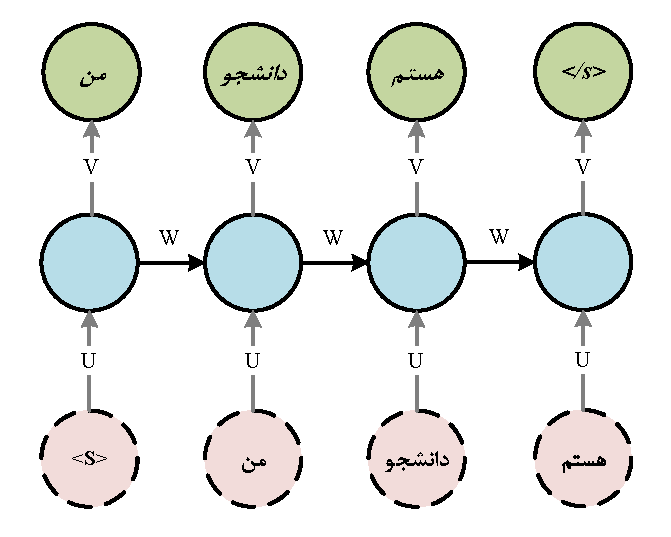
\includegraphics[width=0.7\textwidth, clip=true,  trim= 0 0 0 0]{chapter2/ch2_nlm_persian_crop.pdf}
  	%\includegraphics[width=\textwidth]{figs/chapter1/ch1_fuzz_testing_flowchart2.png}
  	\caption[مدل زبانی عصبی مکرر]
  	{
  		طرح‌واره‌ای از معماری یک مدل زبانی ایجاد شده با استفاده از \gls{RNN}. $ <s> $ نشانه شروع توالی و $ </s> $ نشانه خاتمه توالی در ابتدا و انتهای هر توالی موجود در مجموعه آموزش قرار داده می‌شود. بدین ترتیب، تولید توالی جدید پس از پیش‌بینی نشانه پایان، متوقف می‌گردد \cite{Luong2016}.
  	}
  	\label{ch2_nlm_persian_crop.pdf}
  	%\ref{ch2_nlm_persian_crop.pdf}
  \end{figure}
  
  
  مدل‌های زبانی را \gls{GenerativeModel} نیز می‌نامند؛ زیرا یک توزیع احتمالی روی توالی‌های یک زبان می‌دهند که با نمونه‌‌برداری از آن می‌توان توالی‌های جدید تولید کرد. در \gls{NLP} نشانه‌های هر توالی واژه‌ها هستند، اما می‌توان این مدل را در سطح کاراکتر نیز آموزش داد. ایده اصلی در این پایان‌نامه نیز همین است. هر فایل زبان و قواعد مخصوص به خود را دارد که در مشخصه‌های قالب فایل ذکر شده است. با ایجاد یک مدل زبانی برای این زبان در سطح کاراکتر،  امکان پیش‌بینی نشانه بعدی از روی یک توالی از نشانه‌های داده شده فراهم می‌شود. با نمونه برداری از این مدل زبانی می‌توان داده‌های آزمون جدیدی ایجاد کرد.
 
 \subsection{ارزیابی مدل زبانی}
 چگونه می‌توان میزان خوب بودن یک مدل زبانی را تعیین کرد؟ یک روش برای ارزیابی مدل زبانی، قرار دادن آن در یک وظیفه مشخص و اندازه‌گیری میزان دقت نتایج حاصله است. به این روش‌ \gls{ExtrinsicEvaluation} می‌گویند
 \cite{Jurafsky2017}.
  برای مثال در یک وظیفه تصحیح خودکار غلط‌های املایی، تعداد واژه‌های نادرستی که به‌درستی با واژه‌های صحیح جایگزین شده‌اند را شمارش می‌کنیم و بر تعداد کل واژه‌های غلط تقسیم می‌نماییم. ارزیابی بیرونی، زمان‌بر، پرهزینه و مختص به وظیفه اجرا شده خواهد بود.  روش دیگر استفاده از \gls{IntrinsicEvaluation} است \cite{Jurafsky2017}. معیار \gls{Perplexity} با هدف ارزیابی  درونی مدل زبانی، به‌صورت زیر تعریف می‌شود \cite{mikolov2012statistical}:
  
 \begin{equation}\label{ppl}
 \begin{split}
 	PP_{LM}(x) & = \sqrt[n]{\prod_{i=1}^n(\frac{1}{p(x^{(i)}|<x^{(1)}, ..., x^{(i-1)}>)}} \\
 	& = 2^{-\frac{1}{n}\sum_{i=1}^n\log_{2}{p(x^{(i)}|<x^{(1)}, ..., x^{(i-1)>})}}
 \end{split}
 \end{equation}
در رابطه 
\ref{ppl}،
$ x $
 توالی مورد ارزیابی است. همان‌طور که مشاهده می‌شود \gls{Perplexity} در ارتباط مستقیم با \gls{CrossEntropyError} (رابطه \ref{CrossEntropyLossFunction}) است که میزان اختلاف بین مدل و نمونه‌های مجموعه آزمون را نشان می‌دهد. بنابراین هرچه‌قدر میزان سرگشتگی پایین‌تر باشد، مدل زبانی بهتر است. پایه توان و پایه لـــگاریتم در رابطه \ref{ppl} می‌تواند مقادیری به‌غیر از 2 انتخاب شود. اما در هر حالت هر دو پایه بایستی یکسان باشند تا تساوی اول (بالا) و دوم (پایین) رابطه برقرار گردد. معمولاً از پایه لگاریتم طبیعی در این رابطه استفاده می‌شود 
\cite{DBLP:journals/corr/AbadiABBCCCDDDG16}.

برای درک بهتر نحوه ارزیابی توسط این معیار، توالی 
$ x = <x^{(1)}, x^{(2)}, x^{(3)}, ..., x^{(n)}> $
را در نظر می‌گیریم که متشکل از $ V $ نشانه متفاوت است. $ V $ مجموعه \gls{Vocabulary} زبان است. در غیاب مدل زبانی (بدترین حالت)، تنها می‌توانیم ادعا کنیم که هر نشانه دست‌کم با احتمال 
$ \frac{1}{V} $
در توالی رخ می‌دهد (\gls{BranchingFactor}). بدیهی است که این احتمال برای همه نشانه‌ها یکسان است. برای توالی $ x $ پس از جایگزینی احتمال آن در رابطه  \ref{ppl} داریم:
\begin{equation*}
PP_{LM}(x) = \sqrt[n]{\prod_{i=1}^n(\frac{1}{\frac{1}{V}})} = \sqrt[n]{V^{n}} = V
\end{equation*} 
 بنابراین در بدترین حالت میزان سرگشتگی برابر با اندازه مجموعه \gls{Vocabulary} زبان است. حال چنان‌چه از مدل زبانی استفاده کنیم، احتمال نسبت داده شده به وقوع هر نشانه، نسبت به حالت عدم استفاده از مدل زبانی، افزایش و در نتیجه سرگشتگی کاهش خواهد یافت. در ارزیابی مدل‌های این پایان‌نامه از معیار سرگشتگی استفاده می‌کنیم. 
 
 
 
 
 
 
 \section{خلاصه}
 در این فصل مفاهیم اولیه سه حوزه کلی مطرح در این پایان‌نامه یعنی آزمون نرم‌افزار، آزمون فازی و یادگیری ژرف را بیان کردیم. آزمون نرم‌افزار به‌عنوان یک مسئله تصمیم‌ناپذیر تعریف گردید و معیارهای پوشش برای ارزیابی آن معرفی شدند. آزمون فازی به عنوان یک فن مطرح در آزمون نرم‌افزار، معرفی و از سه دیدگاه مختلف مورد طبقه‌بندی و بحث قرار گرفت: نخست، از دیدگاه اطلاعات در دسترس از \gls{SUT} به سه دسته آزمون جعبه سیاه، جعبه سفید و جعبه خاکستری تقسیم گردید. دوم، از دیدگاه روش‌های تولید داده آزمون به سه دسته مبتنی بر جابه‌جایی، مبتنی بر تولید و نیز ترکیبی تقسیم‌بندی شد. سوم، با توجه به دریافت بازخورد از نتیجه اجرا به دو دسته دارای بازخورد و بدون بازخورد تفکیک گشت. ابزار خودکارسازی آزمون فازی تحت عنوان کلی فازر معرفی و معماری آن تشریح شد.  فازرها با توجه به طبقه‌بندی‌های فوق در بحث آزمون فازی و نیز با توجه به نوع ورودی \gls{SUT} متفاوت هستند. فازرهای قالب فایل مربوط به برنامه‌هایی با ورودی فایل هستند. برای اطلاعات بیشتر در زمینه آزمون نرم‌افزار خواننده را به
  \cite{ammann2016introduction, PaulC.Jorgensen2014} 
 ارجاع می‌دهیم. در زمینه آزمون فازی نیز خواننده را به
 \cite{Chen2018, Mcnally2012, Sutton:2007:FBF:1324770}      
 رجوع می‌دهیم.
 
 در بخش پایانی این فصل، یادگیری ژرف به عنوان زیرشاخه‌ای از یادگیری ماشینی با استفاده از شبکه‌های عصبی مصنوعی، تفهیم شد. شبکه عصبی مورد استفاده در یادگیری ژرف را شبکه عصبی ژرف گویند. \gls{RNN} نوع خاصی از شبکه‌های عصبی ژرف است که برای پردازش وظیفه‌های مبتنی بر توالی مثل مدل زبانی استفاده می‌شود. ساختار یک قالب فایل زبان مختص به خود را دارد و هدف از مطرح کردن اصول اولیه یادگیری ژرف استفاده از مدل‌های این فن، در یادگیری ساختار فایل، جهت تولید داده آزمون جدید است که در فصل 4 به آن خواهیم پرداخت. الگوریتم‌های آموزش شبکه‌های عصبی ژرف ریاضیات گسترده‌ای دارد که به‌طور خلاصه به موارد مهم آن اشاره شد. جهت مطالعه مبسوط این الگوریتم‌ها خواننده را به
 \cite{Goodfellow-et-al-2016}
 ارجاع می‌دهیم. همچنین توضیح کاملی از روش‌های یادگیری توالی با استفاده از \gls{RNN}ها در 
 \cite{DBLP:journals/corr/Lipton15}
 آمده است. در فصل بعد برخی از تازه‌ترین کارهای مرتبط با مفاهیم مطرح شده در این فصل توضیح داده می‌شوند.   
 
 
 
 
 
 
  % فصل دوم: ادبیات موضوع %
% !TeX root=maintext.tex
% !TeX TS-program = XeLaTeX
% !TEX spellcheck = fa
% chapter3

\chapter{روش پیشنهادی}\label{chapter:3}
\thispagestyle{empty}

عنوان این فصل می‌تواند «روش پیشنهادی» یا «فن پیشنهادی» یا «طرح پیشنهادی» یا موارد مشابه باشد و شامل شرح كامل روش/ فن/ طرح ارائه شده خواهد بود.


 \section{معرفی روش يا متدولوژی مورد استفاده}
 
 
  \section{تشريح كليات روش/فن/طرح پيشنهادی}
  
  
   \section{تشريح جزئيات يا اجزاء روش/فن/طرح پيشنهادی }
   
   
  
   \section{خلاصه}
    % فصل سوم: سنجش و بهبود آزمون‌پذیری کد منبع و طراحی نرم‌افزار %
% !TeX root=_main_.tex
% chapter4

\chapter{روش پیشنهادی}\label{ch:4}
\thispagestyle{empty}


\epigraph{
	«اولین قانون هر فناوری مورد استفاده در یک کسب‌وکار این است که اِعمال خودکارسازی به یک عملیات کارآمد، کارآمدی را افزایش می‌دهد. دومین قانون این است که اِعمال خودکارسازی به یک عملیات ناکارآمد، ناکارآمدی را افزایش می‌دهد.»
}
{$ \maltese $ {\large بیل گیتس}}

\noindent
هدف، در روش پیشنهادی همان‌طور که پیش‌ از این هم گفته شد، ایجاد یک مدل برای یادگیری خودکار گرامر قالب فایل و سپس استفاده از آن در تولید داده‌های آزمون جدید است. معماری مدل یادگیرنده ساختار فایل، نحوه آموزش، مجموعه داده لازم برای آموزش مدل، نحوه تولید داده‌های آزمون و در نهایت چگونگی انجام آزمون فازی، مباحثی هستند که در این فصل به آنها خواهیم پرداخت. در ابتدا به بیان کلیات روش پیشنهادی پرداخته و سپس هریک از مراحل را با جزئیات تشریح می‌کنیم.


\section{کلیات}
شکل \ref{ch4_zakeri_proposed_method_flowchart_crop.pdf} یک روندنمای ساده از کلیات مراحل انجام روش پیشنهادی ما را نشان می‌دهد. در ساختار برخی قالب‌های فایل پیچیده مانند \gls{PDF}، بسیاری از قسمت‌ها به صورت متنی هستند. اما ممکن است قسمت‌های دودویی هم وجود داشته باشد. در روش پیشنهادی خود ما ابتدا کلیه قسمت‌های متنی فایل‌های موجود در دانه‌های اولیه را استخراج، سپس این قسمت‌ها را به یکدیگر الحاق می‌کنیم. حاصل این کار ایجاد یک \gls{Corpus} بزرگ است که در بطن خود مشخصه‌های قالب یک فایل را دارد. در ادامه این مجموعه را مطابق با ضوابط فنون یادگیری ماشینی به سه مجموعه آموزش، ارزیابی و آزمون تقسیم‌بندی با نسبت‌های مشخص می‌کنیم. سپس یک مدل مولد را ایجاد و آن را روی داده‌های مجموعه آموزش، با تعریف یک روش یادگیری، آموزش می‌دهیم. در نهایت از این مدل برای ایجاد داده‌های آزمون جدید و اعمال آزمون فازی استفاده خواهیم کرد. اما چون مدل صرفاً قادر به تولید داده‌های متنی است در هنگام ایجاد یک داده آزمون، با فنونی که در ادامه خواهیم گفت، قسمت‌های دودویی را نیز به داده آزمون تزریق می‌نماییم. 


%% برای رعایت قاعده ارجاع به جلو بایستی از پرچم ht در محیط‌های شناور لاتک استفاده کرد.
% h means here: Place the figure in the text where the figure environment is written.
% t means top: Place it at the top of a page.
% b means bottom: Place it at the bottom of a page.
% p means page: Place it on a page containing only floats.
\begin{figure}%[ht]%[tbh!]%%[t!]
	\centering
	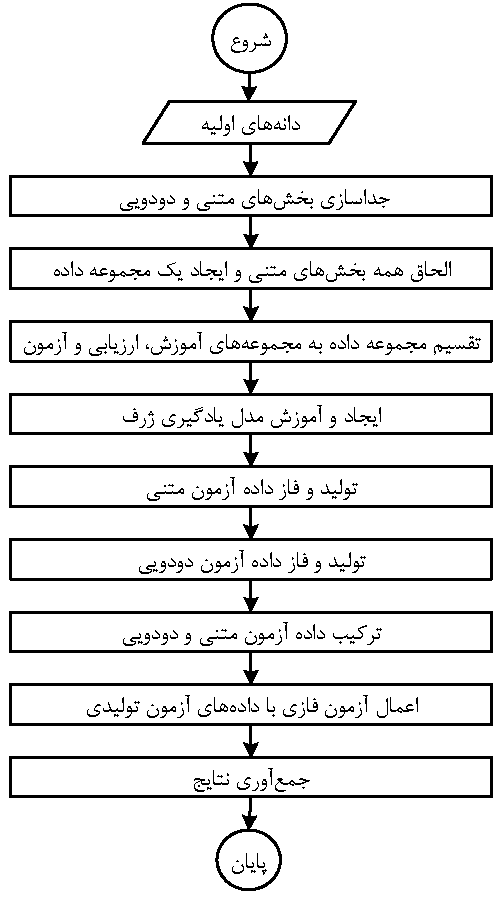
\includegraphics[width=0.7\textwidth, clip=true,  trim= 0 0 0 0]{chapter4/ch4_zakeri_proposed_method_flowchart_crop.pdf}
	%\includegraphics[width=\textwidth]{figs/chapter1/ch1_fuzz_testing_flowchart2.png}
	\caption[روندنمای روش پیشنهادی در حالت کلی]
	{
		روندنمای روش پیشنهادی در حالت کلی.
	}
	\label{ch4_zakeri_proposed_method_flowchart_crop.pdf}
	%\ref{ch4_zakeri_proposed_method_flowchart_crop.pdf}
\end{figure}


\subsection{تمایز داده‌های متنی و دودویی}
گفتیم مدل مولد را روی بخش متنی قالب فایل ایجاد می‌کنیم. اما مفهوم دقیق متنی و دودویی و معیار جداسازی آنها چیست و دلیل تأکید ما بر این موضوع از کجا نشئت می‌گیرد؟ منظور از داده‌های متنی در اینجا مجموعه کدهای \gls{ASCII} است. هنگامی که درسطح بیت یک فایل را بررسی می‌کنیم تمایزی میان واژه‌های متنی و دودویی نیست؛ زیرا همه چیز با مفهوم صفر و یک بیان می‌شود که دودویی است. اما اگر فایل را به‌صورت یک توالی از بایت‌ها در نظر بگیریم، با توجه به اینکه هر بایت 255 حالت ممکن خواهد داشت، می‌توانیم آن فایل را یک زبان متشکل از تکرار حداکثر 255 نشانه بدانیم. کدهای  \gls{ASCII} حتی این تعداد را به 128 نشانه که کاراکترها و نشانه‌های متداول زبان انگلیسی هستند، محدود می‌کنند. مشکل بخش‌های دودویی آن است که اغلب در سطح بیت تفسیر می‌شوند و یادگیری وابستگی‌های آنها با شبکه‌های عصبی، که داده‌های محدودی را در زمان آموزش می‌بینند، امکان‌پذیر نیست. از طرفی هنگامی که نسبت کوچکی از داده‌ها به‌صورت دودویی در میان قسمت‌های متنی ظاهر می‌شوند می‌توان آنها را با روش‌های جابه‌جایی تصادفی فاز کرد.

ما در روش پیشنهادی خود داده‌های دودویی را از قالب فایل حذف کرده اما به‌جای آن یک توکن خاص موسوم به \gls{BinaryToken} را جایگزین می‌کنیم. بدین ترتیب در فرایند آموزش مدل توزیع آماری نحوه ظاهر شدن قسمت‌های دودویی نیز فراگیری می‌شود. حال در فرایند تولید داده‌های آزمون جدید مدل مکان‌های احتمالی ظاهر شدن قسمت دودویی را با پیش‌بینی وقوع توکن مربوطه، تعیین می‌کند. سپس توکن را با یک قسمت دودویی که به‌صورت تصادفی (یا هر روش دیگر) فاز شده است جایگزین می‌کنیم. یعنی وارون عملی که پیش از فرایند آموزش انجام دادیم را پس از فرایند تولید، انجام می‌دهیم. با کلیت گفته شده در اینجا یک روش ترکیبی تولید خودکار داده آزمون خواهیم داشت.


\subsection{تمایز داده و فراداده}\label{sec:data_and_metadata}
در فصل \ref{chapter1}، تمایز داده و فراداده به عنوان یک مسئله در تولید داده آزمون مطرح گردید. مدل مطرح در روش پیشنهادی این امکان را فراهم می‌کند تا بتوانیم به‌صورت احتمالی داده و فراداده را از یکدیگر تشخیص دهیم. از آنجایی که فراداده‌ها در ساختار یک فایل از پیش‌ تعریف شده و تقریباً ثابت هستند، تکرار آنها به مراتب بیشتر از تکرار داده‌ها است که محتویات یک فایل را تشکیل می‌دهند. مدل بدین ترتیب در توزیع آماری یادگیری شده احتمال بیشتری را به فراداده‌ها نسبت می‌دهد. با تعیین یک آستانه مشخص برای هریک از انواع داده و فراداده در هنگام تولید داده آزمون قادر به تصمیم‌گیری در مورد نوع آنها هستیم. ما نتیجه این تصمیم را در نحوه فاز داده آزمون جدید به‌کار می‌بریم، بدین صورت که دو الگوریتم فاز با اهداف فاز فراداده برای مرحله تجزیه و فاز داده برای مرحله پرداخت فایل ارائه خواهیم داد.     


\subsection{مثال انگیزشی}
تمرکز اصلی ما در روش پیشنهادی، بر روی پیمانه تولید داده آزمون در یک فازر قالب فایل است. شکل \ref{ch4_motivating_example}، مراحل تولید داده آزمون از طریق روش پیشنهادی را روی قالب فایل \lr{PDF}، نشان می‌دهد. سه مرحله اصلی در این شکل وجود دارد که به ترتیب با شماره‌های یک تا سه، شماره‌گذاری شده‌اند. مطابق این مراحل، ابتدا پیکره‌ای از فایل‌های از پیش موجود و معتبر جمع آوری گردیده و به عنوان مجموعه داده انتخاب می‌شوند. در مرحله اول، یعنی پیش‌پردازش، هریک از فایل‌های ورودی پیمایش شده، بخش‌های متنی آن جدا و به یکدیگر الحاق می‌شوند. همچنین بخش‌های دودویی داخل فایل، نیز به‌صورت مجزا، پس از جدا شدن، نگهداری می‌شوند. در فایل \lr{PDF}، بخش‌هایی دودویی بین کلیدواژه‌های 
\lr{stream} و \lr{endstream}
می‌آیند که در پیش‌پردازش آنها را با توکن دودویی 
\lr{stream}
جایگزین می‌کنیم. خروجی این مرحله دو مجموعه است. یک مجموعه داده متنی و یک مجموعه داده دودویی. در مجموعه داده متنی، مکان قسمت‌های دودویی با توکن دودویی مشخص شده است.

در مرحله دوم، یک مدل زبانی عصبی برروی مجموعه داده حاصل از جداسازی بخش‌های متنی پیکره آموزش داده می‌شود. مانند هر وظیفه یادگیری ماشینی در این مرحله ابتدا مجموعه داده ورودی به سه مجموعه آموزش، آزمون و ارزیابی تقسیم می‌گردد. خروجی این مرحله یک مدل مولد است که قادر به تولید داده‌های جدید با پیروی از توزیع حاکم بر داده‌های مجموعه آموزش بوده و کاراکتر به کاراکتر داده‌های جدید را تولید می‌کند.

مرحله سوم با روش‌هایی اقدام به تولید داده‌های آزمون جدید، در این‌جا فایل‌های 
\lr{PDF}،
می‌کند. در این مرحله بخش‌های متنی فایل جدید از طریق مدل مولد، یعنی با روش مبتنی بر تولید، ایجاد می‌گردد. عمل بدشکل کردن داده‌های متنی نیز همزمان با تولید آنها صورت می‌گیرد. بدین صورت که برخی از کاراکترها بعد از تولید، بر اساس شرایطی که در ادامه فصل توضیح داده می‌شوند، با کاراکترهای دیگری جایگزین می‌شوند. در همین مرحله، بخش‌هایی دودویی نیز در صورت پیش‌بینی توسط مدل مولد، با یک روش مبتنی بر جابه‌جایی، تولید و در مکان مناسب خود قرار می‌گیرند. منظور از پیش‌بینی در اینجا، تولید توکن دودویی 
\lr{stream}
در توسط مدل مولد است. در تولید بخش دودویی یک داده‌ آزمون از بخش‌های دودویی پیکره اولیه که در مرحله یک جداسازی شده است به‌عنوان دانه اولیه استفاده می‌کنیم. در واقع آنها را با یکی از عملگر‌های جابه‌جایی که در فصل 
\ref{chapter2}
 به آن اشاره شد به‌سادگی جابه‌جا کرده و یک داده آزمون دودویی جدید و فاز شده می‌سازیم. 

مرحله سوم در مجموع تعدادی داده آزمون را با روشی ترکیبی، تولید می‌کند. این داده‌های آزمون سپس می‌توانند به عنوان داده‌های آزمون در فرایند آزمون فازی استفاده شوند. همچنین می‌توان از آن به عنوان دانه اولیه برای فازرهای قالب فایل مبتنی بر جابه‌جایی نیز استفاده کرد. برای ارزیابی روش پیشنهادی خود که در فصل بعد به آن خواهیم پرداخت، در انتهای این فصل یک فازر قالب فایل ساده را مطرح می‌کنیم. این فازر قادر است تا پس از تولید داده‌های آزمون به روش شرح داده شده آنها را به عنوان ورودی به 
\gls{SUT}
تزریق کرده و خطاهای احتمالی را در صورت وجود گزارش کند. مرحله پیش‌پردازش بسیار ساده بوده و نیاز به توضیح خاصی ندارد. این مرحله ممکن است برای قالب‌های فایل مختلف، کاملاً متفاوت باشد. مثلاً برای قالب‌های فایل متنی مثل
\lr{HTML}و \lr{XML}
پیش‌پردازش تنها الحاق کردن کلیه فایل‌های موجود در پیکره است. مراحل دوم و سوم، یعنی ایجاد و آموزش مدل مولد و تولید و فاز داده آزمون، به ترتیب در بخش 
\ref{sec:model}
 و بخش 
 \ref{sec:neural_fuzzing_algorithms}
 توضیح داده شده‌اند. همچنین معماری فازر قالب فایل پیشنهادی در بخش 
 \ref{sec:implementation}
 %\sethlcolor{cyan}\hl{بیان شده است.}
بیان گردیده است.


 

\begin{figure}
	\centering
	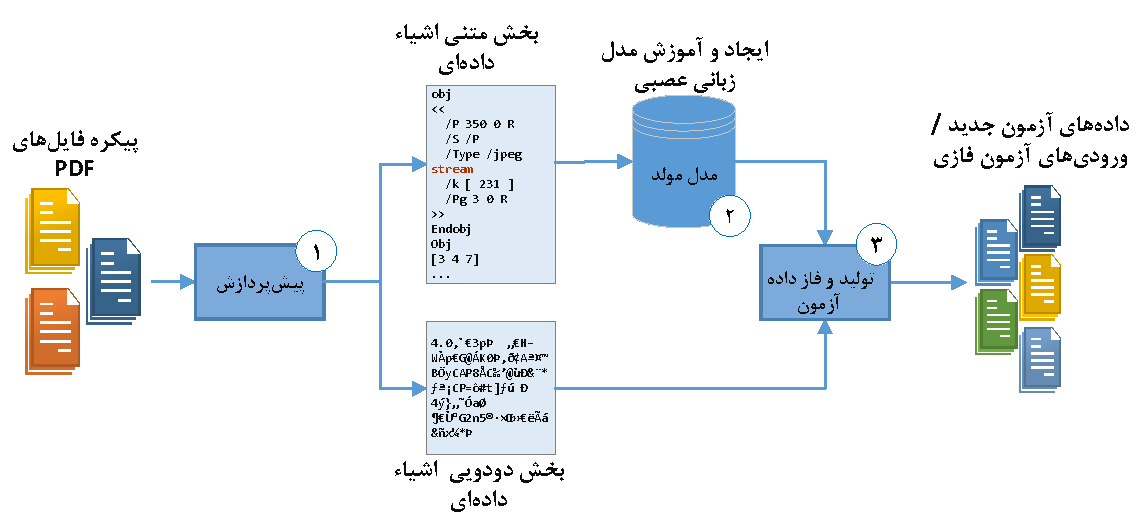
\includegraphics[width=1.0\textwidth, clip=true,  trim= 0 0 0 0]{chapter4/ch4_motivating_example_crop.pdf}
	\caption[مراحل یادگیری ساختار فایل، تولید و فاز داده آزمون برای فایل \lr{PDF}]
	{
		مراحل یادگیری ساختار فایل، تولید و فاز داده آزمون برای فایل \lr{PDF}. 
	}
	\label{ch4_motivating_example}
	%\ref{ch4_motivating_example}
\end{figure}


\section{مدل}\label{sec:model}
یک فایل را می‌توان نمونه تولید شده توسط زبانی که قالب آن فایل را بیان می‌کند دانست. با این فرض می‌توان یک مدل زبانی برای هر قالب فایلی ایجاد کرد. مدل زبانی عصبی عملکرد بهتری نسبت به مد‌های زبانی سنتی دارد. با توجه به ذات مبتنی بر توالی بایت‌های یک فایل، وابستگی بایت فعلی به یک توالی از بایت‌‌های قبلی و نیز تجزیه ترتیبی (چپ به راست و بالا به پایین) آن توسط تجزیه‌گر \gls{SUT} در بسیاری از موارد، در روش پیشنهادی خود، از \gls{RNN} برای ایجاد مدل زبانی و یادگیری ساختار فایل استفاده می‌کنیم. در فصل \ref{chapter2} دیدیم که \gls{RNN} برای یادگیری وظایف مبتنی بر توالی ابداع شده است. به‌طور دقیق‌تر در هنگام آموزش از یک مدل \gls{RNN} چند به یک، با معماری شکل \ref{ch2_karpathy_rnn_crop.pdf} (پ) استفاده خواهیم کرد و در هنگام تولید داده‌ جدید با فراخوانی همین مدل به‌صورت متوالی، مدلی از نوع شکل \ref{ch2_karpathy_rnn_crop.pdf} (ت) خواهیم داشت.

هدف \gls{RNN} در اینجا ایجاد یک مدل زبانی عصبی روی ساختار فایل با دیدن یک پیکره از نمونه‌های آموزشی است. مطابق آنچه گفتیم، مدل زبانی مدلی مولد است، یعنی پس از آموزش، می‌توان از آن برای تولید داده‌های آزمون جدید استفاده کرد، که در ادامه نحوه این کار را توضیح خواهیم داد. در این پایان‌نامه دو مدل با معماری مختلف بر مبنای \gls{RNN} می‌سازیم. در هسته عصب‌های \gls{RNN} هر دو مدل از سلول \gls{LSTM} استفاده می‌کنیم که قابلیت یادگیری توالی‌های با طول زیاد را دارد. مدل اول \gls{LSTM} \gls{Unidirectional} نام دارد که معماری آن مشابه شکل \ref{ch2_rnn.pdf} است. مدل دوم \gls{LSTM} \gls{Bidirectional} است.

\gls{LSTM}
دوسویه توالی ورودی را به دو صورت \gls{Forward} و  \gls{Backward} می‌بیند. در واقع \gls{LSTM} \gls{Bidirectional} از دو \gls{LSTM} یک‌سویه تشکیل شده است. یکی از آنها توالی را از چپ به راست پردازش می‌کند و دیگری از راست به چپ. در نتیجه هر گذرجلو \gls{LSTM} دو خروجی خواهد داشت. یک \gls{MergeFunction} برای ادغام خروجی هریک از \gls{LSTM}های روبه‌جلو و روبه‌عقب به‌کار می‌رود. \gls{MergeFunction} می‌تواند هر تابعی که قادر به ترکیب دو بردار با طول‌های یکسان است، درنظر گرفته شود؛ از جمله: جمع، ضرب، الحاق و غیره. ما از \gls{MergeFunction} جمع برای مدل پیشنهادی خود استفاده می‌کنیم که درایه‌های نظیر به نظیر هر یک از بردارهای خروجی را با یکدیگر جمع می‌زند.

علاوه‌بر نوع مدل \gls{LSTM}، برای \gls{LSTM} یک‌سویه مدل‌هایی با تعداد عصب‌های متفاوت و نیز تعداد لایه‌های پنهان متفاوت را ساخته‌ایم. هدف از این کار مشاهده تأثیر مدل‌های با پیچیدگی مختلف در یادگیری ساختار فایل و تولید داده‌های آزمون و آزمایش این فرضیه است که آیا مدل‌های پیچیده‌تر، مدل‌های ساده‌تر را شکست می‌دهند؟ یعنی موفق به افزایش پوشش کد و یا شناسایی خطاهای بیشتری می‌شوند یا خیر. جـدول \ref{tabel:deep_model} مدل‌های طراحی شده برای استفاده در آزمایش‌های روش پیشنهادی و مشخصه‌های هریک را نشان می‌دهد. یکی از مهم‌ترین مشخصه‌ها تعداد پارامترهای هر مدل است. گراف محاسباتی هریک از مدل‌های جدول \ref{tabel:deep_model} در شکل‌های \ref{ch4_keras_model_archs_crop.pdf}الف تا \ref{ch4_keras_model_archs_crop.pdf}ت آمده است. اندازه ماتریس‌های ورودی و خروجی در گراف مرتبط با تعداد لایه‌های پنهان و نیز تعداد عصب‌ها در هر لایه است که در ادامه بیشتر توضیح داده خواهد شد. همچنین در ادامه پایان‌نامه، هریک از مدل‌های معرفی شده، با شماره ذکر شده برای آنها در جدول 
\ref{tabel:deep_model}
شناخته می‌شوند.

\begin{table}%[ht]
	\caption{مدل‌های یادگیری ژرف طراحی شده، پارامترها و ابرپارامترهای آنها.}
	\label{tabel:deep_model}
	\centering
	\onehalfspacing
	\begin{tabularx}{\textwidth}{r l r r r}
		
		\toprule[1.5pt] شماره (نام) مدل 
		& نوع (معماری) مدل 
		& تعداد لایه  پنهان
		 & تعداد عصب در هر لایه
		  & تعداد پارامترها
		\\
 		\midrule[1.5pt] 1 &  \makecell[l]{\lr{Unidirectional LSTM} \\ \lr{(Many to One)}} & 1 & 128 & 127584
 		\\
 		%\hline 
 		2 & \makecell[l]{\lr{Unidirectional LSTM} \\ \lr{(Many to One)}} & 2 & 128 & 238656
 		\\
 		%\hline 
 		3 & \makecell[l]{\lr{Unidirectional LSTM} \\ \lr{(Many to One)}} & 2 & 256 & 870464
 		\\
 		%\hline 
 		4 & \makecell[l]{\lr{Bidirectional LSTM} \\ \lr{(Many to One)}} & 2 & 128 & 469056
 		\\
 		\bottomrule[1.5pt]
 
	\end{tabularx} 
\end{table}


\begin{figure}%[ht]%[tbh!]%%[t!]
	\centering
	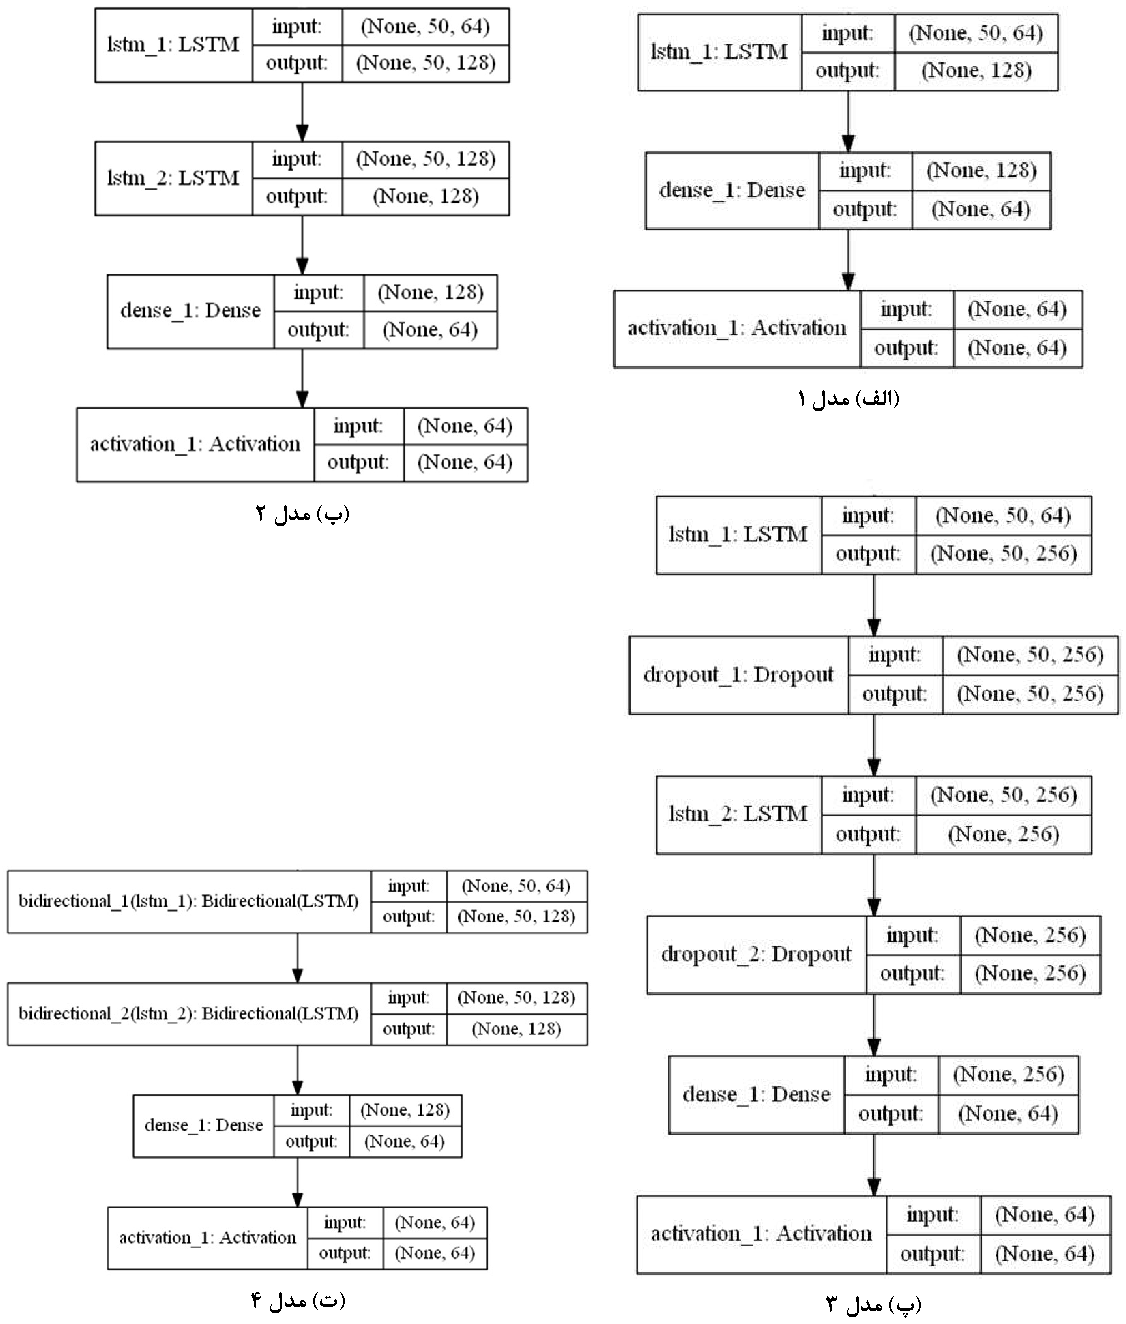
\includegraphics[width=\textwidth, clip=true,  trim= 0 0 0 0]{chapter4/ch4_keras_model_archs_crop.pdf}
	\caption[گراف محاسباتی مدل‌های عصبی ژرف جدول \ref{tabel:deep_model}]
	{
		گراف محاسباتی مدل‌های عصبی ژرف جدول \ref{tabel:deep_model}. اعداد داخل مستطیل‌ها اندازه ماتریس‌های ورودی و خروجی هر لایه را نشان می‌دهند. گراف‌ها با استفاده از توابع کتابخانه \lr{Keras} \cite{chollet2015keras} تولید شده‌اند.  
	}
	\label{ch4_keras_model_archs_crop.pdf}
	%\ref{ch4_keras_model_archs_crop.pdf}
\end{figure}



\subsection{آموزش مدل}

فرایند آموزش همه مدل‌های جدول \ref{tabel:deep_model} یکسان است. در واقع برای آموزش هر مدل تنها نیاز داریم که ورودی و خروجی شبکه عصبی ژرف را مشخص نماییم. پس از استخراج مجموعه داده اولیه که حاوی یک پیکره متوالی از کاراکترهای در بردارنده فایل است، آن را به مجموعه‌های آموزش، آزمون و ارزیابی تقسیم می‌کنیم. چون خروجی مدل مولد در هربار اجرا یک توالی خواهد بود، طول توالی‌های مجموعه داده معیار مناسبی برای تقسیم‌بندی آن به مجموعه‌های سه‌گانه یاد شده است به ‌نحوی که هر مجموعه توزیع یکسانی از فراوانی طول‌های مختلف باشد. از مجموعه‌های آموزش و ارزیابی در هنگام آموزش مدل و از مجموعه آزمون در هنگام تولید داده‌های جدید از روی مدل، استفاده خواهیم کرد. تفکیک مجموعه داده به سه مجموعه آموزش، ارزیابی و آزمون در وظایف یادگیری ماشینی یک امر بدیهی است، اما استفاده از آن برای آزمون فازی و تولید داده‌های آزمون جدید تا قبل از این، انجام نشده و چنان‌چه در ادامه خواهیم دید، ایده جدیدی است. در واقع ما از داده‌های مجموعه آزمون برای تولید داده‌های آزمون جدید استفاده خواهیم کرد.

هر مجموعه بدین ترتیب حاوی تعدادی فایل است و هر فایل یک توالی از کاراکتر‌های \lr{ASCII} است. شروع و پایان هریک از این توالی‌ها پیش از فرایند آموزش، با توکن‌های شروع و پایان که نشانه‌های مجزایی (بیرون از مجموعه داده) هستند برچسب‌گذاری‌ می‌شود. البته بسیاری از قالب‌های فایل چنین توکن‌هایی را به‌عنوان بخشی از ساختار خود دارند. برای مثال فایل‌های \lr{HTML} با برچسب $ <html> $ شروع و با برچسب $ </html> $ خاتمه می‌یابند. فایل‌های \lr{XML} و \lr{PHP} نیز چنین هستند. در این حالت نیازی به افزودن توکن‌های شروع و پایان جدید نیست و می‌توان از همین توکن‌ها استفاده کرد. دلیل افزودن توکن‌های شروع و پایان در این مرحله، به نحوه ساخت مدل‌های زبانی عصبی باز‌ می‌گردد. در واقع این مدل‌ها با دیدن توکن آغازین پیش‌بینی را شروع و با تولید توکن پایانی، پیش‌بینی را خاتمه می‌دهند.

%دلیل این امر همان‌طور که در بخش \ref{sec:language_model} دیدیم، نحوه ساخت مدل‌های زبانی با استفاده از شبکه‌های عصبی است.  

به‌منظور آموزش هر مدل چند به یک و ایجاد یک مدل زبانی عصبی، ابتدا با الحاق محتوای فایل‌های مجموعه آموزش، یک توالی بزرگ از کاراکترها به‌شکل  
$ S = <s^{(1)}, s^{(2)}, s^{(3)}, ..., s^{(n)}> $
 ایجاد می‌کنیم. سپس این توالی را به تعدادی توالی ورودی کوچکتر با طول ثابت $ d $ می‌شکنیم طوری که $i$امین توالی ورودی برابر است با:
 \begin{equation}\label{rel:input_sec}
 	x_i=S[i*j:(i*j)+d]
 \end{equation}
  
  در رابطه 
  \ref{rel:input_sec}،
  $s[l,u]$
   برشی از توالی $s$ بین شاخص‌های $l$ و $u$ بوده و $j$ میزان پرش به جلو در انتخاب توالی ورودی بعدی از توالی اصلی را نشان می‌دهد. ابرپارامتر $d$
   در اینجا، در واقع همان بردار زمینه در مدل زبانی است.
   انتخاب $d$ به پارامترهایی مانند فاصله وابستگی‌های بین بایت‌های مختلف در یک فایل و طول فایل‌های مجموعه‌ داده، بستگی دارد. وقتی از 
   \gls{LSTM}
   به عنوان بلوک‌های سازنده 
   \gls{RNN}
   در ساخت 
   \gls{NLM}
   استفاده شود، می‌توان وابستگی‌های طولانی‌تر را به خوبی یاد‌ گرفت. 
   در عمل و برای وظایف مدل زبانی، این مقدار را بین 40 تا 100 نشانه در نظر می‌گیرند.
   
   گفتیم شبکه عصبی در حالت بانظارت آموزش می‌بیند؛ یعنی، برای هر ورودی یک برچسب خروجی نیاز است. در اینجا کاراکتر بعدی، که هدف پیش‌بینی آن است، را به عنوان برچسب خروجی برای هر توالی ورودی نسبت می‌دهیم. بنابراین برچسب خروجی برای $i$امین توالی ورودی برابر خواهد بود با:
   \begin{equation}
   	 Y_{x_{i}} = S[(i*j) + d+1]
   \end{equation}
     
     
     پس از تولید همه نمونه‌های آموزشی و برچسب‌های متناظر آنها، مدل به صورت انتهابه‌انتها  %\LTRfootnote{\lr{End-to-End}}
     آموزش داده می‌شود؛ مشابه روش یادگیری و فاز
     \cite{Godefroid:2017:LML:3155562.3155573}.
     . یعنی، داده‌های خام مجموعه آموزش، بدون استخراج هیچ‌گونه ویژگی خاصی به شبکه داده می‌شوند و در زمان استفاده نیز، شبکه داده‌های نهایی را بدون نیاز به هیچگونه پسا‌پردازشی تولید می‌کند. در این حالت مدل قادر پیش‌بینی مقدار احتمال شرطی 
     $p(x^{(i+d+1)}| <x^{(i)}, ..., x^{(i+d)}>)$
     خواهد بود. روند تولید نمونه‌های آموزشی در الگوریتم \ref{alg:produce_training_samples} نشان داده شده است. همچنین شکل \ref{ch4_html_toy_example_crop.pdf}، یک فایل \lr{HTML} و سه‌توالی آموزشی اول تولید شده برای آن توسط الگوریتم \ref{alg:produce_training_samples} را به همراه موقعیت قرارگیری آنها در شبکه نشان می‌دهد. توالی ورودی کلی در این مثال، همه کاراکترهای فایل \lr{HTML} و پارامترهای $d$  و $j$ به‌ترتیب برابر 3 و 1 قرار داده شده‌اند. مقادیر در نظر گرفته شده کاملاً فرضی هستند.

شبکه عصبی با مقادیر عددی کار می‌کند. بنابراین بایستی یک نمایش عددی برای هر کاراکتر در مجموعه آموزش در نظر گرفت. یک روش مرسوم در مدل‌های مبتنی بر کاراکتر استفاده از بردارسازی \lr{One-hot} یا $1$ از $k$ است. در این روش یک بردار به  طول اندازه مجموعه واژگان برای هر کاراکتر درنظر می‌گیرند که تنها یکی از شاخص‌های آن برابر $1$ است. بدین ترتیب برای نمایش $V$ کاراکتر، $V$ بردار متفاوت خواهیم داشت. در اینجا نیز از همین روش استفاده می‌کنیم. 

خروجی شبکه نیز که به‌شکل یک کاراکتر تعریف شده است در واقع یک بردار \lr{One-hot} است. در فرایند آموزش تنها یکی از شاخص‌های این بردار یک است. اما در مرحله آزمون بردار تولیدی حاوی مقادیر حقیقی مختلفی در بازه
 $(-\infty, +\infty)$
  برای هر شاخص است. با اعمال تابع بیشینه هموار (رجوع شود به رابطه \ref{softmaxformula})، در خروجی این لایه، می‌توان خروجی را به یک توزیع احتمالی معتبر تبدیل کرد.


\begin{algorithm}%[ht]
	\onehalfspacing
	\caption{\lr{ProduceTrainingSamples}} \label{alg:produce_training_samples}
	\begin{latin}
		\DontPrintSemicolon
		\setcounter{AlgoLine}{0}
		\LinesNumbered
		
		\SetKwFunction{List}{List} 
		\SetKwFunction{Len}{Len} 

		
		\SetKwInput{KwData}{Input}
		\SetKwInput{KwResult}{Output}
		
		\KwData{Total sequence $S$, Input sequences lenght $d$, Jump step $j$}
		\KwResult{Input sequences $x$, Output labels $Y$}
		
		\BlankLine
		
		$x$ $\gets$	\List{} \tcc*{Make an empty list}\; 
		
		$Y$ $\gets$ \List{} \tcc*{Make an empty list}\;
		
		\For{$i \gets 1$ \KwTo \Len{$S$} $ - d $ }{
			
			$x[i] \gets S[i*j:(i*j)+d]$
		
			$Y[i] \gets S[(i*j) + d+1]$
		
	}
	\textbf{Return}	$x$, $Y$

	\end{latin}
\end{algorithm}


\begin{figure}%[ht]%[tbh!]%%[t!]
	\centering
	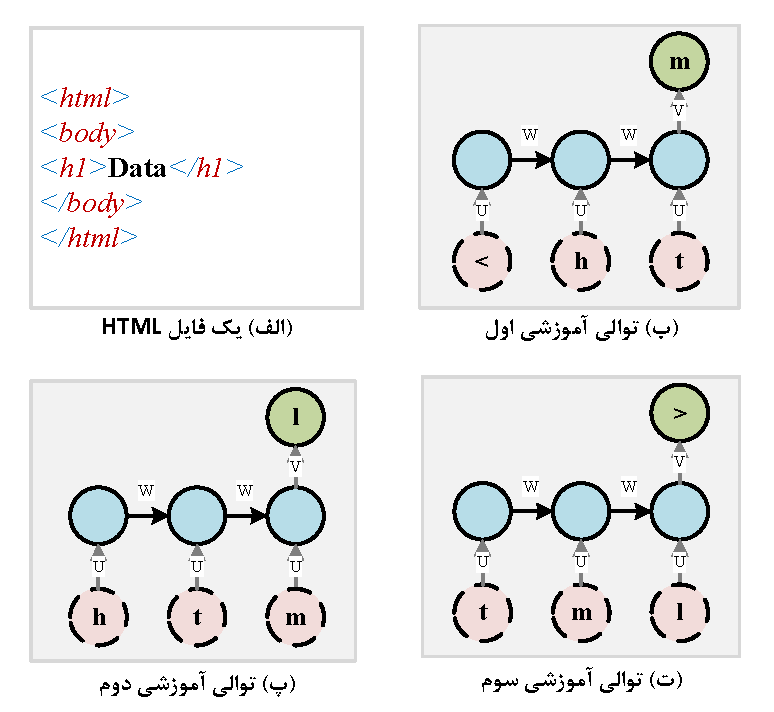
\includegraphics[width=0.95\textwidth, clip=true,  trim= 0 0 0 0]{chapter4/ch4_html_toy_example_crop.pdf}
	\caption[مثالی از نحوه آموزش مدل‌های چند به یک]
	{
		مثالی از نحوه آموزش مدل‌های چند به یک روی یک فایل \lr{HTML} ساده. تنها سه‌توالی آموزشی اول در این شکل نشان داده شده است. اما الگوریتم 4-1 کل فایل را به توالی‌های آموزشی تقسیم می‌کند.
		
		%فراداده‌ها با قلم مورب و داده‌ها با قلم پررنگ مشخص و از یکدیگر متمایز شده‌اند.
	}
	\label{ch4_html_toy_example_crop.pdf}
	%\ref{ch4_html_toy_example_crop.pdf}
\end{figure}



\subsection{تولید داده‌های جدید}\label{sec:generate_new_data}
پس از اتمام فرایند آموزش، مدل برای تولید داده‌های جدید مورد پرس‌وجو قرار می‌گیرد. در این مرحله ابتدا یک پیشوند ثابت از کاراکترهای شروع کننده یک توالی از \textbf{فایل‌های مجموعه آزمون} به طول $d$، که توکن شروع در ابتدای آن است،  به شبکه خورانیده می‌شود\footnote{دقت شود که ویژگی فایل‌های مجموعه آزمون آن است که قبلاً در فرایند آموزش توسط مدل مشاهده نشده‌اند و این امر تأثیر مستقیمی در ارزیابی خوب بودن مدل و تنوع داده‌های تولید شده توسط مدل دارد. بدون وجود مجموعه آزمون نمی‌توانیم معیارهایی مانند سرگشتگی را به‌درستی حساب کنیم. به‌همین سبب جداسازی مجموعه آزمون را تأکید می‌کنیم.}. شبکه توزیع احتمالی کاراکتر $ d+1 $ام را به‌عنوان خروجی تولید می‌کند که شامل یک بردار \lr{One-hot} از مقادیر احتمال‌های تمام کاراکترهای دیده شده هنگام آموزش است. سپس یک کاراکتر از این توزیع احتمالی، انتخاب شده و به پیشوند ورودی الحاق می‌گردد. در این حالت طول پیشوند $d+1 $ است. در مرحله بعد سمت چپ‌ترین کاراکتر پیشوند حذف شده و $d$ کاراکتر باقی مانده دومرتبه به شبکه داده می‌شود تا توزیع احتمالی کاراکتر $d+2 $ حاصل شود. این روند تا زمان تولید توکن پایانی که خاتمه یافتن یک توالی را پیش‌بینی می‌کند، ادامه خواهد داشت. در \cite{Godefroid:2017:LML:3155562.3155573} سه راهبرد تولید داده جدید از توزیع احتمالی پیش‌بینی شده توسط مدل معرفی شده که در بخش \ref{sec:new_data_generation} آنها را دیدیم. 

در اینجا ما از راهبرد نمونه‌برداری که روشی مرسوم برای تولید داده از یک توزیع آماری است استفاده می‌کنیم. یعنی هر بار از توزیع احتمالی پیش‌بینی شده به عنوان یک توزیع \gls{MultinomialDistribution} نمونه‌برداری می‌نماییم. البته راهبردهای جدیدی را نیز معرفی خواهیم کرد. در زبان پایتون و با استفاده از بسته \lr{numpy} می‌توان به‌صورت زیر از یک توزیع چندجمله‌ای نمونه برداری کرد:\newline

\begin{LTR}
	\begin{lstlisting}[language=python, caption={\rl{نمونه‌برداری از توزیع چندجمله‌ای در پایتون.}}, label={codesnip3}]
	import numpy as np
	sample = np.random.multinomial(n, prob_vals, size=None) \end{lstlisting}
\end{LTR}

\subsubsection{پارامتر تنوع}\label{subsec:diversity}
در \cite{Godefroid:2017:LML:3155562.3155573} انتخاب حریصانه به‌دلیل وجود پیشوند ثابت راهبرد ناکارمدی معرفی شده است. در روش پیشنهادی ما، مدل پیشوند‌های متغیری را می‌پذیرد. بنابراین می‌توانیم از راهبرد حریصانه هم استفاده نماییم. با این حال تعداد داده‌های تولیدی در این راهبرد محدود به تعداد نمونه‌های مجموعه آزمون است که البته تعداد کمی نخواهند بود.

در مقابل راهبرد حریصانه، نمونه‌برداری باعث ایجاد اشیای متنوع می‌شود که لزوماً خوش‌شکل نیستند. به‌همین دلیل پارامتری به‌نام \gls{Diversity} را با هدف کنترل داشتن برروی تنوع داده‌های تولیدی مطرح می‌کنیم.  تنوع $D$ به‌صورت یک عدد حقیقی در بازه $(0,+\infty)$ تعریف می‌گردد. در هنگام آزمون مدل، مقادیر حقیقی پیش‌بینی شده توسط مدل، ابتدا بر $D$ تقسیم می‌شوند و سپس تابع بیشینه همواره به آن اعمال می‌شود تا بردار خروجی حاصل گردد. در نتیجه هرچه‌قدر مقدار $D$ کوچک‌تر (نزدیک به صفر) انتخاب شود، نمونه‌برداری به راهبرد حریصانه نزدیک شده، داده‌های خوش‌شکل‌تری تولید می‌گردد اما از تنوع آن کاسته می‌شود. بالعکس هرچه قدر مقدار $D$ بزرگتر از یک انتخاب شود، اختلاف بین مقادیر پیش‌بینی شده کم، تنوع داده‌های تولید شده زیاد و متقابلاً احتمال بد‌شکل بودن آنها افزایش می‌یابد.


\subsubsection{\lr{n}-فهرست بهتر}
یک راهبرد دیگر تولید داده جدید، استفاده از \lr{n}-فهرست بهتر است. در این راهبرد در هر بار پیش‌بینی مدل پس از اعمال تابع بیشینه هموار، تعداد $n$ احتمال بالای بردار خروجی انتخاب و نگهداری می‌شود. سپس با‌ هریک از این احتمال‌ها پیش‌بینی‌ مرحله بعد انجام می‌شود. برای انتخاب \lr{n}-فهرست بهتر بین دو پیش‌بینی مقادیر احتمال‌های هر دو فهرست در یکدیگر ضرب و $n$ حاصل‌ضرب بالاتر انتخاب می‌شود. پس از $B$ مرحله، $n$ پیشــوند $B$تـایی خواهیم داشت که پیشوند با بالاترین احتمال پیشوند خروجی خواهد بود. این راهبرد البته زمان و حافظه مصرفی بالایی نیاز دارد. لذا مقادیر $n$ و $B$ بایستی کوچک انتخاب شوند. در ترجمه ماشینی معمولاً از این راهبرد نیز استفاده می‌شود. ما در این پایان‌نامه و در آزمایش‌های خود، راهبرد بالا را ارزیابی نکردیم، اما می‌توان از آن در عمل استفاده کرد.  

\section{الگوریتم‌های فاز عصبی}\label{sec:neural_fuzzing_algorithms}
این بخش را می‌توان هسته روش پیشنهادی و نوآوری‌های ارایه شده در این پایان‌نامه دانست. در اینجا توضیح می‌دهیم که داده‌های آزمون چگونه با روشی خودکار و ترکیبی تولید و فاز می‌شوند. هنگامی که داده‌های آزمون را با استفاده از مدل‌های بخش \ref{sec:model} و راهبردهای معرفی شده در بخش \ref{sec:generate_new_data} تولید می کنیم یک تنوع ذاتی در داده‌ها وجود خواهد داشت و در هر صورت داده‌های آزمون جدید محسوب می‌شوند. اما اهداف یادگیری قالب فایل و آزمون فازی قالب فایل در تضاد بایکدیگر هستند. هدف الگوریتم یادگیری ایجاد داده‌های خوش‌شکل است که بتواند از تجزیه‌گر اولیه عبور و مسیرهای عمیق را اجرا کند و هدف آزمون فازی بد‌شکل کردن ورودی است به‌نحوی که تجزیه‌گر و دیگر قسمت‌های کد اجرا شده را به حالت خرابی ببرد. در این بخش، ما الگوریتم‌های فاز عصبی را با هـدف ایجاد یک مصالحه بین دو هدف قبلی و تولید نهایی داده آزمون برای یک فازر قالب فایل، معرفی می‌کنیم. 

فاز کردن داده آزمون همزمان با تولید آن از روی مدل صورت می‌گیرد و مرحله مجزایی نیست. الگوریتم‌های \ref{alg:data_neural_fuzz} و \ref{alg:metadata_neural_fuzz} نحوه تولید داده آزمون که در بخش \ref{sec:generate_new_data} بحث شد و فاز همزمان آن را نشان می‌دهند. هر دو الگوریتم به‌عنوان ورودی مدل یادگیری شده $M$، پیشوند شروع توالی $P$ (حاوی توکن شروع)، تنوع نمونه‌برداری $D$، نرخ فاز $FR$، توکن پایان $ET$ و توکن دودویی $BT$ را پذیرفته و داده آزمون $TD$ را به‌عنوان خروجی باز می‌گردانند.

حلقه اصلی هر یک از الگوریتم‌ها، تا زمانی که $ET$ تولید نشده باشد ادامه‌ می‌یابد. چنان‌چه طول توالی تولید شده از یک حد آستانه
 $MaxLen$
 بیشتر شد ولی 
 $ET$ 
 کماکان تولید نشده باشد، آنگاه $ET$ به‌صورت خودکار به انتهای $TD$ اضافه می‌شود تا الگوریتم از حلقه تکرار بیرون آید. بدین ترتیب مطمئن می‌شویم که الگوریتم هموراه خاتمه خواهد یافت. سپس در صورتی که مدل حضور یک داده دودویی در $TD$ را پیش‌بینی کرده باشد (یعنی $BT$ در توالی $TD$ پیدا شود)، ابتدا یک بخش دودویی جایگزین $BT$ شده و سپس این بخش با روش‌های جابه‌جایی تصادفی یا هر روش دلخواه دیگر به‌صورت مجزا فاز می‌شود و در نهایت داده آزمون نهایی توسط الگوریتم بازگردانیده می‌شود. ما در عمل برای خط 19 هر دو الگوریتم، عملگر معکوس کردن یک بایت را در نظر گرفتیم. بدین ترتیب که درصد ثابتی از بایت‌های دودویی را در هر بخش دودویی انتخاب شده، به‌صورت تصادفی انتخاب نموده و مقادیر بیت‌های هر بایت انتخابی را معکوس می‌کنیم.
 
 \subsection{فاز عصبی داده}
 
 تفاوت اصلی در الگوریتم‌های فاز عصبی داده و فاز عصبی فراداده در هنگام اعمال عملیات فاز است. در بخش \ref{sec:data_and_metadata} گفتیم مدل به داده‌ها احتمال کمتری نسبت می‌دهد. بنابراین در الگوریتم \ref{alg:data_neural_fuzz}، هرگاه احتمال کاراکتر پیش‌بینی شده از یک حد آستانه
  $\alpha$
  کمتر باشد، متوجه می‌شویم که کاراکتر جزو بخش داده فایل بوده که در این حالت آن را با کاراکتری که کمترین احتمال را دارد جایگزین می کنیم. با این امید که کم‌احتمال‌ترین کاراکتر، ناخواسته‌ترین کاراکتر نیز بوده و ممکن است منجربه‌ خرابی شود.
   
  
  خط 7 الگوریتم \ref{alg:data_neural_fuzz} بیان می‌دارد که برای فاز بایستی شرایط دیگری علاوه بر شرط فوق برقرار باشد. از جمله عدد تصادفی 
  $p\_fuzz$
  که لازم است از $FR$ یعنی نرخ فاز کمتر شود. هرچه‌قدر مقدار $FR$ بزرگتر انتخاب شود شرط $p\_fuzz<FR$ برای اعداد بیشتری تحقق می‌یابد. بدین ترتیب آزمون‌گر می‌تواند روی درصد کاراکترهای فاز شده کنترل داشته باشد. %در آزمایش‌ها ما پارامتر $FR$ را برابر 0.1 قرار دادیم.
  همچنین می‌خواهیم که مجموعه کاراکترهای توالی‌های $ET$ و $BT$ فاز نشود؛ زیرا از آنها در قسمت‌های بعد استفاده می‌کنیم. لذا دو شرط دیگر به شرط‌های خط 7 الگوریتم \ref{alg:data_neural_fuzz} اضافه می‌شوند. بنابراین فاز کاراکتر پیش‌بینی شده تنها در حالتی که ترکیب عطفی هر 4 شرط درست باشد، صورت می‌گیرد.
  
  تغییر یک بایت یا یک کاراکتر از بخش‌های داده یک فایل، معمولاً بدشکل بودن خاصی را ارائه نمی‌دهد. به طور شهودی تصور کنید که به جای عدد 125 عدد 925 قرار داده شود یا هر البته هر کاراکتر دیگری در موقعیت رقم 1. در بد شکل کردن داده هدف ما جایگزین کردن یک مقدار مرزی به جای داده موجود است. مثلاً برای مورد گفته شده جایگذاری عددی به فرم
   $999 . . . 9$ 
   خوب به نظر می‌رسد. در واقع در فاز عصبی داده، به دنبال روشی برای انتشار فاز به کاراکترهای بعدی نیز هستیم.
  وقتی یک کاراکتر فاز شد، دو راهکار برای تولید کاراکترهای بعدی پیش‌رو داریم. راهکار اول تولید کاراکترهای بعدی، مستقل از کاراکتر فاز شده است؛ یعنی اینکه مدل در تولید کاراکتر $t$ام هیچ آگاهی از فاز شدن کاراکتر مرحله 
  $t-1$ام 
  خود نداشته باشد. برای این منظور کافی است تا کاراکتر اولیه تولید شده توسط مدل، یعنی کاراکتر قبل از فاز  و جایگزین شدن، را به پیشوند شروع توالی $P$ اضافه کنیم. بدین ترتیب مدل مستقل از اینکه کاراکتر فاز شده است یا نه به تولید داده‌های مبتنی بر گرامر (داده‌های خوش‌شکل) ادامه می‌دهد. راهکار دوم تولید کاراکترهای بعدی، وابسته به کاراکتر فاز شده است؛ یعنی اینکه اثر کاراکتر فاز شده به کاراکترهای تولید شده در مراحل بعد سرایت کند. برای این منظور کاراکتر فاز شده را به پیشوند شروع توالی         
  $P$
  اضافه کرده و مدل را به سمت بد شکل کردن کاراکترهای بعدی متمایل می‌کنیم. این راهکار در الگوریتم فاز عصبی داده به دلیل شرح داده شده استفاده گردیده است. خط 10 الگوریتم 
  \ref{alg:data_neural_fuzz}،
  کاراکتر فاز شده یعنی کاراکتر 
  $c$
  را به پیشوند 
  $P$
  اضافه می‌کند. در همین خط برای ثابت ماندن طول پیشوند که در واقع ورودی مدل است، کاراکتر اول یعنی قدیمی‌ترین کاراکتر را از پیشوند حذف می‌کنیم. در کل این خط عمل 
  \textbf{انتشار فاز به جلو}
  را پیاده‌سازی می‌کند.
 
 
 
\subsection{فاز عصبی فراداده}
در الگوریتم فاز عصبی فراداده (الگوریتم \ref{alg:metadata_neural_fuzz})، می‌خواهیم کاراکترهای فراداده را تغییر دهیم. برای این منظور بررسی می‌کنیم که احتمال کاراکتر پیش‌بینی شده توسط مدل یعنی $p(c)$ بیشتر از حد آستانه 
$\beta$
باشد، در این صورت کاراکتر با کمترین احتمال را جایگزین می‌کنیم. در اینجا اما به‌دنبال تغییر تنها یکی از کاراکترها در هر توکن فراداده هستیم. لذا در خط 11 الگوریتم \ref{alg:metadata_neural_fuzz} تغییری در پیشوند بعدی مدل ایجاد نمی‌کنیم تا مدل به همان روند تولید داده خوش‌شکل خود ادامه دهد بدون اینکه متوجه فاز شدن کاراکتر پیش‌بینی کرده گام زمانی قبلی خود باشد. در واقع در فاز عصبی فرا داده، انتشار فاز به جلو را انجام نمی‌دهیم. ایده ما برای این کار این است که در اغلب مواقع یک تغییر کوچک، مثلاً تغییر یک بایت در قسمتی که قالب فایل را بیان می‌کند سبب گمراه شدن تجزیه‌گر می‌شود. این عمل درست در خلاف مورد داده است که یک بایت معمولاً تغییری ایجاد نمی‌کند و این مقادیر مرزی (بیش از حد کوچک، بیش از حد بزرگ، خالی یا صفر) هستند که مسبب خرابی می‌شوند. مقادیر داده معمولاً به‌صورت یک توالی از بایت‌ها ادامه می‌یابند. 


در الگوریتم \ref{alg:metadata_neural_fuzz} پارامتر نرخ فاز $FR$ همچنان وجود دارد، اما دو شرطی که بررسی کننده وجود توکن‌های $BT$ و $ET$ هستند را حذف کردیم تا علاوه بر آسان‌تر کردن شرط فاز بتوانیم آنها را نیز به‌عنوان بخشی از قالب فایل، فاز کنیم؛ زیرا، تعداد خطاهایی که در تجزیه‌گر رخ می‌دهند، معمولاً بیشتر هستند.
در نهایت خطوط سایه زده شده در الگوریتم \ref{alg:metadata_neural_fuzz} (خطوط7، 8 و 11) محل‌های تفاوت این الگوریتم با الگوریتم فاز عصبی داده (الگوریتم \ref{alg:data_neural_fuzz}) را نشان می‌دهد.
 
 حد آستانه $MexLen$ که حداکثر طول داده آزمون تولیدی را در الگوریتم‌های \ref{alg:data_neural_fuzz} و \ref{alg:metadata_neural_fuzz} مشخص می‌کند نیز به‌صورت یک عدد صحیح تصادفی در بازه $[a,b)$ مشخص می‌شود. مقادیر این بازه می‌تواند براساس میانگین طول فایل‌های مجموعه آزمون، انتخاب شود. بدین صورت که کران‌های آن برابر اختلاف واریانس طول از میانگین باشند. مقادیر ابرپارامترهای موجود در هر دو الگوریتم بایستی توسط آزمون‌گر مطابق قالب فایل مورد آزمون و نکته‌های بیان‌ شده، تنظیم گردد. در فصل 
 \ref{ch:5}
 که ارزیابی روش پیشنهادی را مطرح می‌کنیم، مقادیر در نظر گرفته شده را برای قالب فایل 
 \lr{PDF}
 بیان می‌کنیم.
  %در ارزیابی‌ها ما  ابرپارامترهای دو الگوریتم پیشنهادی خود را به‌صورت زیر مقداردهی کردیم:
 %$$\alpha=0.5,\quad \beta=0.9,\quad a=450,\quad b=550$$
 %همچنین پارامتر ورودی $D$ را برابر با هریک از مقادیر $0.5$، $1$ و $1.5$ و پارامتر ورودی $FR$  را برابر $0.1$ قرار دادیم.
 

%%% My algorithms %%%
%%
%% 1 - DataNeuralFuzz
%%
\begin{algorithm}%[ht]
	\onehalfspacing
	\caption{\lr{DataNeuralFuzz}} \label{alg:data_neural_fuzz}
	\begin{latin}
		%\begin{algorithmic}[1]
		\DontPrintSemicolon
		\setcounter{AlgoLine}{0}
		\LinesNumbered
		
		\SetKwFunction{Random}{Random}
		\SetKwFunction{RandInt}{RandInt}
		\SetKwFunction{Predict}{Predict}
		\SetKwFunction{EndsWith}{EndsWith}
		\SetKwFunction{Sample}{Sample}
		\SetKwFunction{Chars}{Chars}
		\SetKwFunction{Len}{Len}
		\SetKwFunction{AddBinaryPart}{AddBinaryPart}
		\SetKwFunction{MutateBinaryPart}{MutateBinaryPart}
		\SetKwInput{KwData}{Input}
		\SetKwInput{KwResult}{Output}
		
		\KwData{Learnt model $M$, Sequence prefix $P$, Diversity $D$, Fuzzing rate $FR$, End token $ET$, Binary token $BT$}
		\KwResult{Test data $TD$}
		
		\BlankLine
		
		$TD$  $\gets$ $P$\;
		
		$MaxLen$  $\gets$ \RandInt($a$, $b$)\;
		
		\While{$not$ \EndsWith($TD$, $ET$)}
		{
			$predicts$  $\gets$ \Predict($M$($P$))\;
			
			$c$, $p(c)$  $\gets$ \Sample($predicts$, $D$) \tcc*{Sample c from the learnt model}\;
			
			$p\_fuzz$  $\gets$ \Random($0,1$) \tcc*{Decide whether to fuzz}\;
			
			\If{ $p\_fuzz<FR \wedge p(c)<\alpha \wedge c\not\in$ \Chars($BT$) $\wedge c\not\in$ \Chars($ET$)}
			{
				$c$  $\gets$ $argmin_{c'}\{ p(c') \in predicts \}$ \tcc*{Fuzz c by c' where c' is the lowest likelihood}\;
			} 
			
			$TD$  $\gets$ $TD$ + $c$\;
			
			$P$  $\gets$ $P[1:]$ + $c$ \tcc*{Propagate fuzz to prefix and next generated data}\;
			
			\If{ \Len($TD$) > $MaxLen$ }
			{
				$TD$  $\gets$ $TD$ + $ET$ \;
				
				\textbf{Break}\;
			}
			
		}
		
		\If {$BT \in TD$}
		{
			$TD$ $\gets$ \AddBinaryPart($TD$)\;
			
			$TD$ $\gets$ \MutateBinaryPart($TD$)\;
		}
		
		\textbf{Return} $TD$\;
		
		%\end{algorithmic}
	\end{latin}
\end{algorithm}


%%
%% 2 - MetadataNeuralFuzz
%%
\begin{algorithm}%[ht]
	\onehalfspacing
	\caption{\lr{MetadataNeuralFuzz}} \label{alg:metadata_neural_fuzz}
	\begin{latin}
		%\begin{algorithmic}[1]
		\DontPrintSemicolon
		\setcounter{AlgoLine}{0}
		\LinesNumbered
		
		\SetKwFunction{Random}{Random}
		\SetKwFunction{RandInt}{RandInt}
		\SetKwFunction{Predict}{Predict}
		\SetKwFunction{EndsWith}{EndsWith}
		\SetKwFunction{Sample}{Sample}
		\SetKwFunction{Chars}{Chars}
		\SetKwFunction{Len}{Len}
		\SetKwFunction{AddBinaryPart}{AddBinaryPart}
		\SetKwFunction{MutateBinaryPart}{MutateBinaryPart}
		\SetKwInput{KwData}{Input}
		\SetKwInput{KwResult}{Output}
		
		\KwData{Learnt model $M$, Sequence prefix $P$, Diversity $D$, Fuzzing rate $FR$, End token $ET$, Binary token $BT$}
		\KwResult{Test data $TD$}
		
		\BlankLine
		
		$TD$ $\gets$ $P$\;
		
		$MaxLen$  $\gets$ \RandInt($a$, $b$)\;
		
		\While{$not$ \EndsWith($TD$, $ET$)}
		{
			$predicts$  $\gets$ \Predict($M$($P$))\;
			
			$c$, $p(c)$  $\gets$ \Sample($predicts$, $D$) \tcc*{Sample c from the learnt model}\;
			
			$p\_fuzz$  $\gets$ \Random($0,1$) \tcc*{Decide whether to fuzz}\;
			
			\HiLi \If{ $p\_fuzz < FR \wedge p(c) > \beta$ }
			{
				\HiLi $c'$  $\gets$ $argmin_{c"}\{ p(c") \in predicts \}$ \tcc*{Fuzz c by c' where c' is the lowest likelihood}\;
			} 
			
			\HiLi $TD$  $\gets$ $TD$ + $c'$\;
			
			$P$  $\gets$ $P[1:]$ + $c$\; \tcc*{Don't propagate fuzz to prefix}
			
			\If{ \Len($TD$) > $MaxLen$ }
			{
				$TD$  $\gets$ $TD$ + $ET$ \;
				
				\textbf{Break}\;
			}
			
		}
		
		\If {$BT \in TD$}
		{
			$TD$  $\gets$ \AddBinaryPart($TD$)\;
			
			$TD$  $\gets$ \MutateBinaryPart($TD$)\;
		}
		
		\textbf{Return} $TD$\;
		
		%\end{algorithmic}
	\end{latin}
\end{algorithm}%

%%%%%%



\section{پیاده‌سازی}\label{sec:implementation}

جزئیات پیاده‌سازی روش پیشنهادی در پیوست \ref{appendix:2} آمده است. برای پیاده‌سازی مدل‌های یادگیری ژرف از کتابخانه سطح بالای یادگیری ژرف \lr{Keras}
\cite{chollet2015keras}  
که به زبان پایتون نوشته شده است استفاده کردیم. این کتابخانه مجموعه‌ای مفید از توابع و \lr{API}ها برای ساخت انواع مختلف شبکه‌های عصبی را در اختیار قرار می‌دهد؛ اما، برای اجرا نیاز به یک چارچوب سطح پایین دارد که ما  \lr{Tensorflow} 
\cite{DBLP:journals/corr/AbadiABBCCCDDDG16}
را بدین منظور انتخاب کردیم. \lr{Tensorflow} همچنین یک ابزار به نام \lr{Tensorboard} دارد که از آن می‌توان برای مصورسازی گراف‌های محاسباتی و نیز مشاهده نمودارهای خطاو دقت در فرایندهای آموزش و آزمون استفاده کرد. برای آموزش مدل‌ها ما از تابع خطای \lr{CE} (رابطه \ref{CrossEntropyLossFunction} در بخش \ref{feedforwardtraining}) و بهینه‌ساز \lr{Adam} 
\cite{DBLP:journals/corr/KingmaB14}
با نرخ‌های یادگیری 
$1 \times 10^{-3}$
و
$1 \times 10^{-4}$
استفاده کردیم.

هدف این پایان‌نامه همان‌طور که پیش از این گفته شد، ارائه یک روش تولید خودکار داده آزمون است که در بخش‌های گذشته این فصل بحث شد. اما تولید داده آزمون به‌تنهایی کافی نیست و برای ارزیابی لازم است تا یک فازر قالب فایل با همه پیمانه‌های شکل \ref{ch2_fuzz_testing_flowchart_crop.pdf} در اختیار داشته باشیم. برای این منظور نیاز به دو پیمانه تزریق کننده مورد آزمون و پایش \gls{SUT} نیز داریم. اغلب نرم‌افزارهایی که یک فایل را به‌عنوان ورودی می‌پذیرند یک واسط خط فرمان نیز دارند که می‌توان از این طریق یک فایل را به آنها داد. در غیر اینصورت نیز می‌توان یک برنامه کوچک برای تزریق ورودی نوشت. به‌طور کلی در آزمون فازی قالب فایل تزریق ورودی ساده است. برای پایش نیز ابزارهای مستقلی وجود دارد که می‌توان از آنها استفاده کرد. ما آزمون فازی را تحت سیستم عامل ویندوز انجام دادیم\footnote{هرچند که روش پیشنهادی کاملاً مستقل از سیستم عامل است. برنامه تولید خودکار داده آزمون به زبان پایتون نوشته شده و روی سکوهای مختلف قابل اجرا است.} و ابزار \lr{Application Verifier} 
\cite{ApplicationVerifier}
که در بخش \ref{sec:fuzzers_architechture} معرفی شد را برای پایش انتخاب کردیم که مایکروسافت استفاده از آن را در \gls{SDL} توصیه کرده است.

\lr{Application Verifier}
فایل اجرایی \gls{SUT} را می‌گیرد و در هر بار اجرای \gls{SUT} یک فایل حاوی وقایع را با یک شماره ترتیبی ثبت می‌کند. در صورتی که برنامه دچار خطای زمانِ ‌اجرا (شامل یکی از انواع خطاهای فساد حافظه، دسترسی غیر مجاز و غیره) شود، نوع خطا در این فایل ثبت و ضبط می‌گردد. سپس می‌توان برنامه را به‌همراه داده آزمون مسبب خطا (که از روی شماره ترتیبی فایل وقایع قابل تشخیص است) در یک محیط اشکال‌زدا مانند \lr{WinDbg} مجدداً اجرا و ضمن مشاهده خطا، محل دقیق آن را آشکار ساخت.

از سازوکاری که در بالا توضیح داده شد برای آزمون فازی نرم‌افزار \lr{MuPDF} که یک نرم‌افزار پر استفاده است و قالب پیچیده \gls{PDF} را به‌عنوان ورودی می‌پذیرد، در آزمایش‌ها استفاده کرده‌ایم. ما همچنین پوشش کد این نرم‌افزار را با استفاده ابزار  \lr{VSPerfMon}  اندازه‌گیری کردیم تا عملکرد تولید کننده داده آزمون را بسنجیم. شکل \ref{ch4_iust_deep_fuzzer_crop.pdf} یک طرح‌واره کلی از معماری (مؤلفه‌ها و ارتباط بین آنها) فازر پیشنهادی ما در این پایان‌نامه را نشان می‌دهد. با تعویض پیمانه‌ پایش، این فازر در سیستم‌های عامل دیگر نیز قابل اجرا خواهد بود. این فازر را می‌توان در گروه فازرهای جعبه خاکستری، مبتنی بر روش ترکیبی تولید داده آزمون و بدون حلقه بازخورد به‌شمار آورد. \lr{VSPerfMon} برای اندازه‌گیری پوشش کد در حالت جعبه‌سفید استفاده می‌شود که در صورت عدم وجود کد منبع \gls{SUT} بایستی آن را با یکی از ابزارهای سنجش پوشش کد باینری در بخش \ref{sec:instrumenting} جایگزین کرد.


\begin{figure}%[ht]%[tbh!]%%[t!]
	\centering
	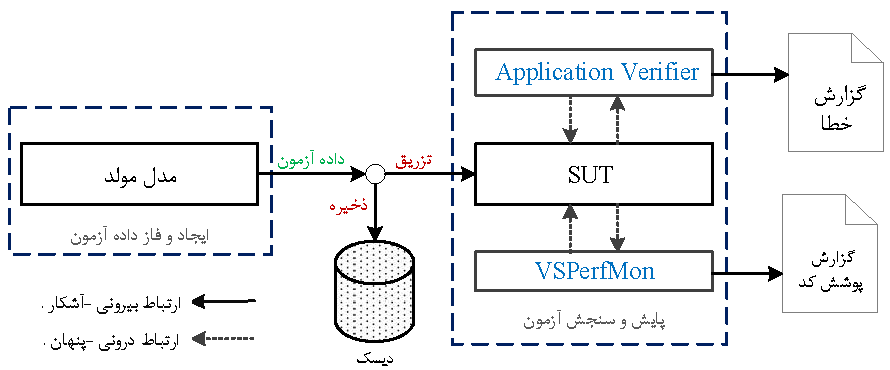
\includegraphics[width=\textwidth, clip=true,  trim= 0 0 0 0]{chapter4/ch4_iust_deep_fuzzer_crop.pdf}
	\caption[معماری فازر قالب فایل پیشنهادی و ارتباط بین مؤلفه‌های مختلف آن]
	{
		معماری فازر قالب فایل پیشنهادی. فازر به‌صورت کاملاً پیمانه‌ای پیاده‌سازی شده است. پیکان‌ها ارتباطات بین مؤلفه‌ها را نشان می‌دهند. ارتباط بیرونی، سازوکار ارتباطی است که توسط ما پیاده‌سازی شده یا قابل تغییر است و ارتباط درونی سازو‌کار ارتباطی است که توسط پیمانه‌های شخص ثالث استفاده می‌شود. 
	}
	\label{ch4_iust_deep_fuzzer_crop.pdf}
	%\ref{ch4_iust_deep_fuzzer_crop.pdf}
\end{figure}




\section{خلاصه}
مدل‌های زبانی عصبی در سطح کاراکتر قابلیت یادگیری یک توزیع آماری روی یک توالی از کاراکترها را دارند. در این فصل ما ساختار یک فایل را به صورت یک توالی از کاراکترها (بایت‌ها) مدل کرده و با ارائه چندین مدل زبانی عصبی و چندین راهبرد تولید داده‌های جدید از این مدل‌ها، یک روش تولید خودکار داده آزمون ارائه دادیم که قابل استفاده در فازرهای قالب فایل مختلف است. ما همچنین دو الگوریتم با عنوان‌های فاز داده عصبی و فاز فراداده عصبی ارائه کردیم. هر کدام از این الگوریتم‌ها بدشکل‌سازی داده آزمون ورودی را با هدف خاصی انجام می‌دهند: اولی با هدف جابه‌جایی داده‌های یک فایل به منظور ایجاد خطا در هنگام پرداخت آنها و دومی با هدف جابه‌جایی فراداده‌های یک فایل برای اینجا خطا در تجزیه‌گر اولیه ساختار فایل تحت فاز. 

در بخش پایانی فصل نیز یک فازر قالب فایل را طراحی و پیاده‌سازی کردیم که از آن می‌توان برای آزمون فازی برنامه‌هایی با ورودی فایل استفاده کرد. خروجی این فازر علاوه بر گزارش خطاهای یافت شده حین فرایند آزمون، گزارش میزان پوشش کد و ذخیره کلیه داده‌های آزمون تولید شده نیز است. معماری فازر پیشنهادی کاملاً پیمانه‌ای بوده و با تعویض پیمانه‌ پایش، امکان استفاده از آن در سیستم‌های عاملی به‌جز ویندوز فراهم می‌شود. فازر معرفی شده یک فازر جعبه خاکستری و مجهز به یک روش تولید داده آزمون ترکیبی است. در فصل \ref{ch:5}، به ارزیابی روش پیشنهادی و بررسی یافته‌های حاصل از آن می‌پردازیم.






 % فصل چهارم: سنجش و بهبود آزمون‌پذیری نیازمندی‌ها %
% !TeX root=maintext.tex
% !TeX TS-program = XeLaTeX
% !TEX spellcheck = fa
% chapter5

\chapter{نتیجه‌گیری و کارهای آتی}\label{chapter:5}
\thispagestyle{empty}

این بخش به بررسی محتوای پایان‌نامه، بیان نوآوری‌ها و جمع‌بندی آن می‌پردازد. هدف ارائه خلاصه‌ای از یافته‌های تحقیق است. این بخش می‌تواند حاوی بیان مختصر مراحل انجام تحقیق باشد. مطالب پاراگراف‌بندی شود و هر پاراگراف به یك موضوع مستقل اختصاص یابد. فقط به ارائه یافته‌ها و دست‌آوردها بسنده شود و از تعمیم بی‌مورد نتایج خودداری شود. از ارائه جداول و نمودارها اجتناب شود. از ارائه عناوین كلی در حوزه‌ی تحقیق و پیشنهاد تحقیقات آتی خودداری شود و كاملاً در چارچوب و زمینه‌ی مربوط به تحقیق جاری باشد. این بخش می‌تواند یك الی سه صفحه باشد. 

\section{کارهای آینده}
در این بخش، عناوین و موضوعات پیشنهادی برای تحقیقات آتی كه كاملاً مرتبط با تحقیق جاری هستند ارائه شود. این بخش در حد یك صفحه باشد. 

 % فصل پنجم: زمان‌بندی پیشنهادی %
\clearpage
 % مراجع %
%\pagestyle{empty}
%\pagestyle{fancy}
%\fancyhead[LE,RO]{\slshape \rightmark}
\fancyhead[LO,RE]{\slshape }
\onehalfspacing
%\fancyhead[LE,RO]{\slshape ک}
%\fancyhead[LO,RE]{\slshape م}
	% تعیین قالب درج مراجع %
\bibliographystyle{ieeetr-fa}%{acm-fa}%{chicago-fa}%{plainnat-fa}%
\bibliography{bibitems/references-all.bib}

%\pagestyle{empty}

\clearpage
% ضمائم %
\appendix % فصل های پس از این قسمت به عنوان ضمیمه خواهند آمد. %
% -- اگر پیوست اول خود را در فایلی به جز appendix1 همراه با این کلاس نوشته‌اید، باید چندخط اول appendix1 را در فایل خود کپی کنید.
%\pagestyle{fancy}
%\fancyhead[LE,RO]{\slshape \rightmark}
\fancyhead[LO,RE]{\slshape \leftmark}
%% !TeX root=_main_.tex
% appendix1
% دستورات زیر باید در اولین فایل پیوست باشند. آنها را حذف نکنید!
\addtocontents{toc}
{
    \protect\renewcommand\protect\cftchappresnum{\appendixname~}%
    \protect\setlength{\cftchapnumwidth}{\mylenapp}
}%
    
\chapter{ساختار فایل PDF}\label{appendix:1}
\thispagestyle{empty}

در این پیوست به‌طور خلاصه ساختار کلی یک فایل \gls{PDF}
 را به‌عنوان یک ساختار فایل پیچیده بیان می‌کنیم. در فصل \ref{chapter1} اشاره کردیم که ویژگی‌های کامل قالب \gls{PDF}
  بسیار زیاد است. بیشتر این ویژگی‌ها، در حدود 70 درصد، در ارتباط با توضیح \glspl{DataObject} و ارتباط آنها بین بخش‌های مختلف یک فایل \gls{PDF}
   هست. تمرکز اصلی در این پیوست نیز بر روی ساختار \glspl{DataObject} خواهد بود. ما ساختار کلی \gls{PDF} را در دو بخش فیزیکی و منطقی بررسی خواهیم کرد.

فایل‌های \gls{PDF}
 در یک قالب متنی کدگذاری می‌شوند که ممکن است شامل \glspl{BinaryStream} مانند تصویر و غیره باشند. یک فایل \gls{PDF}
 ترکیبی از دست‌ِکم یک \gls{Body} است. یک \gls{Body} از سه بخش تشکیل شده است:  \gls{Object} (\lr{obj})، \gls{CrossReferenceTable} (\lr{xref})  و \lr{Trailer}. در ابتدای هر فایل یک سرآیند قرار می‌گیرد که با عبارت \lr{\%PDF} آغاز شده و در ادامه آن یک عدد که نگارش قالب \gls{PDF}
 را مشخص می‌کند، آمده است. ‏شکل \ref{appendix1_pdf_hello_world.png} یک فایل \gls{PDF}
  شامل متن  \lr{Hello Wrold} را که در یک ویراستار متنی باز شده است، نشان می‌دهد. در ادامه این ساختار را بررسی می‌کنیم.



\begin{figure}%[tbh!]%[ht]%[t!]
	\centering
	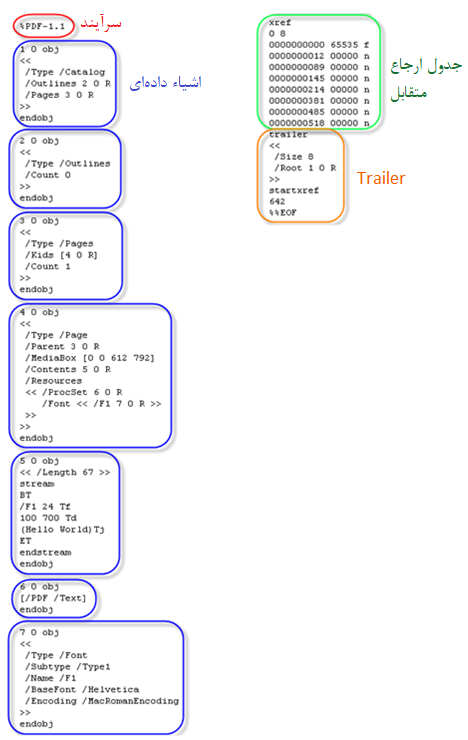
\includegraphics[width=0.8\textwidth, clip=true,  trim= 0 0 0 0]{appendix1/appendix1_pdf_hello_world.png}
	\caption[ یک فایل \gls*{PDF}  باز شده در یک ویراستار متنی شامل عبارت \lr{Hello World}]
	{
		یک فایل ساده \gls*{PDF} باز شده در یک ویراستار متنی شامل عبارت \lr{Hello Wrold}. چپ: سرآیند فایل و اشیای داده‌ای؛ اشیاء با مستطیل آبی (شماره‌های 1 تا 7) مشخص شده‌اند. راست: ادامه محتویات همان فایل، شامل جدول ارجاع متقابل و \lr{Trailer}.
	}
	\label{appendix1_pdf_hello_world.png}
	%\ref{appendix1_pdf_hello_world.png}
\end{figure}


\section{ساختار فیزیکی}\label{sec:physical_structure}
جزئیات ساختار فیزیکی بدنه فایل \gls*{PDF} به شرح زیر است:
\begin{itemize}
	\item{
		\textbf{اشیاء.}	
داده و فراداده در پرونده‌های \gls*{PDF}در یک واحد اولیه که شیء نامیده می‌شود سازماندهی می‌شوند. اشیا همگی قالب مشابهی دارند که در شکل \ref{appendix1_pdf_hello_world.png} مشخص است و همچنین یک ساختار بیرونی مشترک هم دارند. اولین خط یک شیء شناسه آن است که برای ارجاع‌های غیر مستقیم استفاده می‌شود. در ادامه عدد تولیدی آن است که اگر شی با یک نسخه جدیدتر بازنویسی شود، افزایش می‌یابد. سپس رشته 
\texttt{\lr{"obj"}}
 که شروع یک شیء را مشخص می‌کند آمده و پس از آن محتویات شیء قرار داده می‌شود. رشته 
 \texttt{\lr{"endobj"}}
 نیز پایان یافتن محدوده یک شیء را مشخص می‌کند.
	}

	\item{
		\textbf{جدول ارجاع متقابل.}	
	این جدول در بدنه \gls*{PDF} شامل آدرس نسبی اشیای مورد ارجاع قرار گرفته داخل یک فایل به صورت بایت می‌باشد. در شکل \ref{appendix1_pdf_hello_world.png} این جدول شامل 7 شیء با شناسه یک تا 7 و یک مکان نگهدارنده برای شناسه صفر است که به هیچ شیئی اشاره نمی‌کند.
	
	
	}

	\item{
		\textbf{\lr{Trailer}.}	
	 این قسمت از بدنه فایل \gls*{PDF} شامل یک \gls{Dictionary} از اطلاعات بدنه، مثل تعداد کل اشیای داخل فایل 
	 (\texttt{\lr{/size 8}})، شناسه و شماره ترتیبی شیء ریشه 
     (\texttt{\lr{/root 1 0 R}})
	 و غیره است. فرهنگ‌لغت بین نمادهای $ << $  و  $ >> $ قرار می‌گیرد. ادامه \lr{Trailer} شامل \lr{startxref} است که آدرس نسبی شروع جدول ارجاع متقابل در فایل را مشخص می‌کند. این فن اجازه می‌دهد تا بدنه از پایان با خواندن \lr{startxref} پویش شود، سپس به جدول ارجاع متقابل بازگشته و آن را نیز پویش می‌کند. بدین ترتیب تنها اشایی پویش می‌شوند که نیاز هستند. در شکل \ref{appendix1_pdf_hello_world.png} آدرس شروع جدول ارجاع متقابل که پس از \lr{startxref} در \lr{Trailer} آمده است برابر با 642 است. در صورتی که آدرس‌‌های بایت‌های این فایل بررسی شود، مشاهده خواهد شد که بایت 642ام شروع جدول ارجاع متقابل (کاراکتر \texttt{\lr{'x'}}) است. در پایانِ \lr{Trailer} نیز عبارت 
	 \texttt{\lr{\%\%EOF}}
	 قرار می‌گیرد که پایانِ فایل را مشخص می‌کند.
	
	}
\end{itemize}


ساختار جدول ارجاع متقابل و \lr{Trailer} به‌نسبت ساده و در فایل‌های گوناگون مشابه است، اما اشیای \gls{PDF}
 انواع محتلفی دارند. برای مثال شیء شماره 1 در شکل \ref{appendix1_pdf_hello_world.png}، حاوی یک ساختار فرهنگ ‌لغت است لذا بین نمادهای $ << $  و  $ >> $  واقع‌شده و حاوی کلیدهایی می‌شود که با کاراکتر $/$ شروع شده و در ادامه مقادیر آنها آمده است. مثلا مقدار 
\texttt{\lr{2 0 R}}
 یک ارجاع به شیئی در همین فایل با شناسه 2 و شماره ترتیبی 0 است. از آنجایی که یک فایل ممکن است خیلی بزرگ باشد؛ آدرس نسبی شیئی که به آن ارجاع داده شده است از طریق جدول ارجاع متقابل که یک جدول دسترسی تصادفی است، قابل دستیابی خواهد بود.
 
اشیای \gls{PDF}
 تنها محدود به فرهنگ لغت نمی‌شوند گرچه به‌نظر می‌آید که بیشتر آنها دست کم شامل یک فرهنگ لغت هستند. شیء شماره 5 در شکل \ref{appendix1_pdf_hello_world.png} برای نمونه، حاوی یک جریان دودویی است که بین واژه‌های کلیدی \lr{stream} و \lr{endstream} قرار گرفته است. تصاویر داخل \gls{PDF}
  نمونه‌ای از جریان‌های دودویی هستند که به این صورت می‌توانند ظاهر شوند. ‏شکل \ref{appendix1_pdf_stream_object.png}، یک شیء حاوی تصویر را نشان می‌دهد که در یک ویراستار متنی باز شده است.  شیء شماره 6 در شکل \ref{appendix1_pdf_hello_world.png} یک آرایه از کلید‌ها را شامل می‌شود. مقادیر آرایه می‌توانند انواع مختلفی داشته باشند که در هر صورت بین نمادهای $ [$  و $ ] $ قرار می‌گیرند و با کاراکتر فاصله از یکدیگر تمییز داده می‌شوند. به‌دلیل تنوع ذکر شده در ساختار اشیای \lr{PDF}، قواعد تعریف و ترکیب این اشیاء بیشترین بخش از توضیحات مشخصه‌های قالب فایل \gls{PDF}
  را تشکیل می‌دهند.


\begin{figure}%[tbh!]%[ht]%[t!]
	\centering
	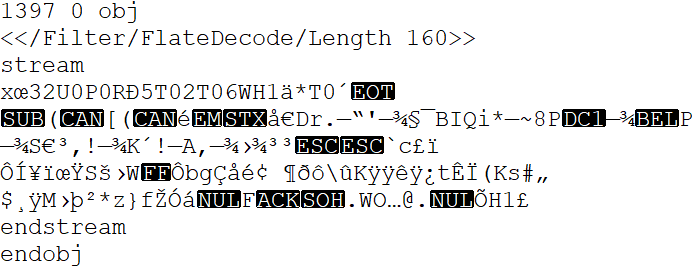
\includegraphics[width=0.9\textwidth, clip=true,  trim= 0 0 0 0]{appendix1/appendix1_pdf_stream_object.png}
	\caption[یک شیء \gls*{PDF} حاوی جریان دودویی]
	{
		یک شی \gls*{PDF}
		 حاوی یک تصویر. محتوای دودویی تصویر بین stream و endstream قرار گرفته است.
	}
	\label{appendix1_pdf_stream_object.png}
	%\ref{appendix1_pdf_stream_object.png}
\end{figure}

 
\section{ساختار منطقی}

آنچه در بخش \ref{sec:physical_structure} صحبت شد مربوط ساختار فیزیکی یک فایل \gls{PDF}
و نحوه قرار گرفتن اجزای فایل در کنار یکدیگر بود (مرتبط با گام پویش در هنگام اجرا). ساختار منطقی فایل \lr{PDF}، یعنی قواعد حاکم بر نحوه تفسیر و پردازش آنچه در یک فایل قرار دارد و ارتباط بین اجزا، یک ساختار سلسله مراتبی است (مرتبط با گام پرداخت در هنگام اجرا). شناسه شیء ریشه در Trailer مشخص می‌شود. به‌همین ترتیب شیء یا اشیای بعدی مورد نیاز در شیء ریشه معلوم می‌گردد. در فایل \gls{PDF}
شکل \ref{appendix1_pdf_hello_world.png} شیء شماره 1 ریشه است. اشیای شماره 2 و 3 داخل بدنه شیء 1 مورد دسترسی قرار می‌گیرند و در نهایت ترتیب نحوه دسترسی‌ها به‌صورت یک درخت قابل نمایش است که ساختار منطقی فایل را نشان می‌دهد. ‏شکل \ref{appendix1_pdf_logical_structure.png} ساختار منطقی فایل نشان داده شده در ‏شکل \ref{appendix1_pdf_hello_world.png} را نشان می‌دهد.


\begin{figure}%[tbh!]%[ht]%[t!]
	\centering
	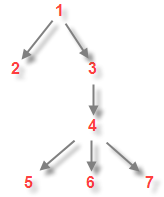
\includegraphics[clip=true,  trim= 0 0 0 0]{appendix1/appendix1_pdf_logical_structure.png}
	\caption[نمایش درختی ساختار منطقی فایل \gls*{PDF}]
	{
		ساختار منطقی فایل \gls*{PDF}
		 نشان داده شده در شکل \ref{appendix1_pdf_hello_world.png}. گره‌های درخت شناسه اشیاء در فایل \gls*{PDF}
		  و یال‌های آن معرف نحوه فراخوانی هر شی‌ء توسط شی‌ء دیگر هستند.
	}
	\label{appendix1_pdf_logical_structure.png}
	%\ref{appendix1_pdf_logical_structure.png}
\end{figure}



ساختار فیزیکی یک فایل \gls{PDF}
 را می‌توان بدون تغییر ساختار منطقی آن، به شکل دیگری تبدیل کرد. برای مثال در شکل \ref{appendix1_pdf_hello_world.png} اشیاء به‌ترتیب صعودی شناسه خود در فایل ظاهر شده بودند. می‌‌شود ترتیب قرارگرفتن اشیاء را به‌صورت نزولی در آورد. در این صورت جدول ارجاع متقابل بایستی بروزرسانی شود؛ زیرا، هر شی در در مکان متفاوتی نسبت به قبل قرار گرفته است. اما این پدیده تأثیری بر ساختار منطقی ندارد. ساختار منطقی کماکان همان ساختار ‏شکل \ref{appendix1_pdf_logical_structure.png} و نتیجه اجرا نیز با فایل قبلی یکسان خواهد بود. جدول ارجاع متقابل برای حالتی که اشیاء به صورت نزولی در فایل ظاهر شده باشند، در ‏شکل \ref{appendix1_xref_updated.png} نشان داده شده است.



\begin{figure}%[tbh!]%[ht]%[t!]
	\centering
	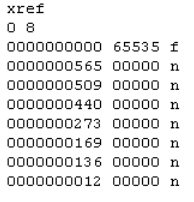
\includegraphics[clip=true,  trim= 0 0 0 0]{appendix1/appendix1_xref_updated.png}
	\caption[جدول ارجاع متقابل بروزرسانی شده یک فایل \gls*{PDF}]
	{
		جدول ارجاع متقابل بروزرسانی شده در حالتی که اشیاء به ترتیب نزولی شناسه خود در فایل \gls*{PDF}
		 ظاهر شده‌اند.
	}
	\label{appendix1_xref_updated.png}
	%\ref{appendix1_xref_updated.png}
\end{figure}



به‌طور کلی اشیاء \gls{PDF}
می‌توانند در مکان‌های تصادفی داخل یک فایل \gls{PDF}
 ظاهر شوند بدون اینکه تأثیر بر پرداخت فایل داشته باشند. برای فایل ساده ‏شکل \ref{appendix1_pdf_hello_world.png} تنها با تعویض ترتیب ظاهر شدن اشیاء می‌توان تعداد 5040 (برابر با !7) فایل با ساختار فیزیکی متفاوت داشت. این درحالی است که تغییر ترتیب قرارگیری اشیا تنها یک روش برای جابه‌جایی ساختار فیزیکی فایل \gls{PDF}
  است و روش‌های دیگری مثل تغییر محل قرارگیری جدول ارجاع متقابل نیز وجود دارد. بنابراین رابطه بین ساختار منطقی و فیزیکی فایل \gls{PDF}
  به صورت یک به چند است.

\section{بروزرسانی فایل PDF}

دیدیم که چگونه ساختار منطقی فایل \gls{PDF}
مستقل از ساختار فیزیکی آن شکل می‌گیرد. بروزرسانی فایل \gls{PDF}
 بر همین مبنا است. فایل‌های \gls{PDF}
 می‌توانند به‌صورت \gls{Incremental} بروزرسانی شوند. بدین ترتیب که اگر نویسنده فایل \gls{PDF}
  بخواهد اطلاعات داخل شیء شماره 7 را بروزرسانی کند، یک بدنه جدید آغاز می‌کند. سپس محتوای شیء جدید را داخل آن نوشته، عدد تولیدی (عدد بعد از شناسه شیء) را یک واحد نسبت به عدد تولیدی شیء قدیم افزایش داده و برای شی جدید می‌نویسد. در  انتها نیز یک جدول ارجاع متقابل را که به شیء جدید اشاره می‌نماید، تولید کرده و بدنه جدید را به سند قبلی الصاق می‌کند.














%% !TeX root=z-main.tex

\chapter{فازر }\label{appendix:2}
\thispagestyle{empty}



%\baselineskip=.75cm
\clearpage

\fancyhead[LO, RE]{\slshape}
\onehalfspacing
\printglossary %Glossary and index %
%\phantomsection
%\addcontentsline{toc}{chapter}{\indexname}
%\printindex
\clearpage
\bookmark[dest=latintitle]{Latin Abstract and Title}
% !TeX root=maintext.tex
% !TeX TS-program = XeLaTeX
% !TEX spellcheck = fa
% Title English
% Latin abtrsaction and other info
% By: Morteza ZAKERI

% در این فایل، عنوان پایان‌نامه، مشخصات خود و چکیده پایان‌نامه را به انگلیسی، وارد کنید.

%%%%%%%%%%%%%%%%%%%%%%%%%%%%%%%%%%%%
\baselineskip=1.25cm

\begin{latin}
	
	\latinuniversity{Iran University of Science and Technology}
	\latinfaculty{School of Computer Engineering}
	\latinsubject{Computer Engineering}
	\latinfield{Software}
	\hypertarget{latintitle}{}
    
	\latintitle{\begin{doublespace}
            Thesis Latin Title
        \end{doublespace}
    }  
    
	\firstlatinsupervisor{Dr. First name Surname }
	%\secondlatinsupervisor{Second Supervisor}
	\firstlatinadvisor{Dr. First name  Surname}
	%\secondlatinadvisor{Second Advisor}
	\latinname{ First name }
	\latinsurname{ Surname }
	\latinthesisdate{February 2021}
	
	\latinkeywords{Keywords}
	\en-abstract{
	Put your latin abstract here.
     %%
}
\latinfirstPage

\end{latin}
 % Thesis english title %


\end{document}